\documentclass[11pt,oneside]{book}
\usepackage{fontspec}
\setmainfont{Noto Serif}
\setsansfont{Noto Sans}
\setmonofont{Noto Sans Mono}
\newfontfamily\proseunicodefont{DejaVu Serif}
\usepackage[margin=1in]{geometry}
\usepackage{microtype}
\usepackage{amsmath,amssymb,amsthm,mathtools,bm}
\usepackage{graphicx}
\usepackage{xcolor}
\usepackage{booktabs}
\usepackage{array}
\usepackage{longtable}
\usepackage{enumitem}
\usepackage{float}
\usepackage{caption}
\usepackage{hyperref}
\usepackage{fancyhdr}
\usepackage{tikz}
\usetikzlibrary{arrows.meta,positioning,calc,decorations.pathmorphing}

\hypersetup{
  colorlinks=true,
  linkcolor=blue!50!black,
  urlcolor=blue!50!black,
  citecolor=blue!50!black
}

\setlength{\parskip}{0.5em}
\setlength{\parindent}{0pt}
\setlist[itemize]{topsep=0.25em,itemsep=0.2em}
\setlist[enumerate]{topsep=0.25em,itemsep=0.2em}
\setlength{\headheight}{40pt}
\numberwithin{equation}{chapter}

\newtheorem{theorem}{Teorema}[chapter]
\newtheorem{proposition}[theorem]{Proposición}
\newtheorem{lemma}[theorem]{Lema}
\newtheorem{corollary}[theorem]{Corolario}
\theoremstyle{definition}
\newtheorem{definition}[theorem]{Definición}
\newtheorem{example}[theorem]{Ejemplo}
\theoremstyle{remark}
\newtheorem{remark}[theorem]{Observación}

\providecommand{\ket}[1]{\left\lvert#1\right\rangle}
\providecommand{\bra}[1]{\left\langle#1\right\rvert}
\providecommand{\braket}[2]{\left\langle#1\,\middle|\,#2\right\rangle}
\providecommand{\expect}[1]{\left\langle#1\right\rangle}
\newcommand{\lectureoverview}[1]{\paragraph{Resumen.} #1}

\makeatletter
\newcommand{\course@headerfont}{\normalfont\small\itshape}
\newcommand{\course@pagefont}{\normalfont\small}
\newcommand{\course@headerraise}{14pt}
\newlength{\course@headerboxheight}
\setlength{\course@headerboxheight}{\dimexpr\headheight-\course@headerraise-9pt\relax}
\newcommand{\course@leftheadbox}[1]{%
  \raisebox{\course@headerraise}{%
    \parbox[t][\course@headerboxheight][t]{0.82\textwidth}{%
      \raggedright\course@headerfont\strut\MakeUppercase{#1}\strut%
    }%
  }%
}
\newcommand{\course@rightheadbox}[1]{%
  \raisebox{\course@headerraise}{%
    \parbox[t][\course@headerboxheight][t]{0.82\textwidth}{%
      \raggedleft\course@headerfont\strut\MakeUppercase{#1}\strut%
    }%
  }%
}
\renewcommand{\chaptermark}[1]{\markboth{\MakeUppercase{\chaptername\ \thechapter.\ #1}}{}}
\renewcommand{\sectionmark}[1]{\markright{\MakeUppercase{\thesection\hspace{0.4em}#1}}}
\fancyhf{}
\fancyhead[L]{\course@leftheadbox{\leftmark}}
\fancyhead[R]{\course@pagefont\thepage}
\renewcommand{\headrulewidth}{0.5pt}
\pagestyle{fancy}
\fancypagestyle{plain}{%
  \fancyhf{}
  \fancyhead[L]{\course@leftheadbox{\leftmark}}
  \fancyhead[R]{\course@pagefont\thepage}
  \renewcommand{\headrulewidth}{0.5pt}
}
\makeatother

% Reader-facing provenance for classroom exchanges and editorial additions.
\newenvironment{classroomqa}{%
  \par\medskip\noindent\begin{minipage}{\linewidth}\small\hrule\medskip
}{%
  \medskip\hrule\end{minipage}\par\medskip
}
\newcommand{\audiencequestion}[1]{\noindent\textbf{Pregunta del público.} #1\par\smallskip}
\newcommand{\lecturerresponse}[1]{\noindent\textbf{Respuesta.} #1\par}
\newcommand{\lecturetimestamp}[1]{\footnote{Marca temporal: #1.}}
\newcommand{\lectureframe}[1]{\par\smallskip{\centering\footnotesize\itshape Fotograma de la clase: #1.\par}}
\newcommand{\editorialnote}[1]{\footnote{Aclaración editorial: #1}}

\usepackage{polyglossia}
\setdefaultlanguage{spanish}
\usepackage{sectsty}
\renewcommand{\contentsname}{Índice}
\renewcommand{\chaptername}{Capítulo}
\renewcommand{\figurename}{Figura}
\renewcommand{\tablename}{Tabla}
\renewcommand{\proofname}{Demostración}
\renewcommand{\bibname}{Bibliografía}
\sectionfont{\raggedright}
\subsectionfont{\raggedright}
\makeatletter
\renewcommand{\@pnumwidth}{2.2em}
\renewcommand{\@tocrmarg}{3.2em}
\makeatother
\usepackage{tocloft}
\renewcommand{\cftchapfont}{\small\bfseries}
\renewcommand{\cftchappagefont}{\small\bfseries}
\renewcommand{\cftsecfont}{\small}
\renewcommand{\cftsecpagefont}{\small}
\setlength{\cftsecnumwidth}{3em}
\renewcommand{\cftsubsecfont}{\small}
\renewcommand{\cftsubsecpagefont}{\small}
\setlength{\cftsubsecindent}{4.5em}
\setlength{\cftsubsecnumwidth}{4em}
\emergencystretch=6em
\pdfstringdefDisableCommands{\def\proseunicodefont{}}

\geometry{paperwidth=177.6mm,paperheight=252mm,left=16mm,right=16mm,
 top=18mm,bottom=18mm,includeheadfoot,headheight=28pt,headsep=7mm,footskip=9mm}
\usepackage{scrextend}
\changefontsizes[17pt]{12pt}
\raggedbottom
\renewenvironment{classroomqa}{\par\medskip\begingroup}{\par\endgroup\medskip}
\fancyhf{}
\setlength{\headwidth}{\textwidth}
\fancyhead[L]{\parbox{\textwidth}{\raggedright\fontsize{9}{11}\selectfont\nouppercase{\leftmark}}}
\fancyfoot[C]{\small\thepage}
\renewcommand{\headrulewidth}{0.3pt}
\fancypagestyle{plain}{\fancyhf{}\fancyfoot[C]{\small\thepage}\renewcommand{\headrulewidth}{0pt}}

\hypersetup{
  pdftitle={Topics in String Theory},
  pdfauthor={Leonard Susskind},
  pdfsubject={Independently edited companion notes for the 2011 Winter lecture course},
  pdfcreator={LaTeX with hyperref}
}
\graphicspath{{../../../generated_course_notes/supplementary/cosmology_and_black_holes/2011_winter_topics_in_string_theory/figures/}{../../../generated_course_notes/supplementary/cosmology_and_black_holes/2011_winter_topics_in_string_theory/assets/}}
\begin{document}
\frontmatter
\hypersetup{pageanchor=false}
\begin{titlepage}
\hyphenpenalty=10000\exhyphenpenalty=10000
\thispagestyle{empty}
\begin{tikzpicture}[remember picture,overlay]
  \node[anchor=center,inner sep=0] at (current page.center) {%
    \includegraphics[height=\paperheight,keepaspectratio]{../../../generated_course_notes/supplementary/cosmology_and_black_holes/2011_winter_topics_in_string_theory/assets/cover-art.png}%
  };
  \node[
    anchor=north west,
    align=left,
    text width=0.78\paperwidth,
    fill=white,
    fill opacity=0.9,
    rounded corners=8pt,
    inner xsep=10pt,
    inner ysep=8pt
  ] at ([xshift=0.08\paperwidth,yshift=-0.06\paperheight]current page.north west) {%
    {\fontsize{30}{33}\selectfont\bfseries\color{black!88} Temas de teoría de cuerdas\\[0.85em]}
    {\large\color{black!72} Edición en español / invierno de 2011, temas de teoría de cuerdas}
  };
  \node[
    anchor=south west,
    align=left,
    text width=0.68\paperwidth,
    fill=white,
    fill opacity=0.82,
    text opacity=1,
    rounded corners=6pt,
    inner sep=12pt
  ] at ([xshift=0.08\paperwidth,yshift=0.08\paperheight]current page.south west) {%
    {\normalsize\color{black!78} Clases originales: Leonard Susskind\\[0.35em]}
    {\small\color{black!72} Edición complementaria: \href{https://lazying.art}{LazyingArt LLC} / \href{https://github.com/lachlanchen/Video2Book}{Video2Book}}
  };
\end{tikzpicture}
\mbox{}
\end{titlepage}
\hypersetup{pageanchor=true}

\clearpage
\chapter*{Sobre estas notas}
Estas notas complementarias, editadas de forma independiente, siguen las clases de Leonard Susskind. Se reconstruyeron a partir de transcripciones automáticas, subtítulos y una selección de fotogramas de la pizarra, y luego se cotejaron con el material fuente disponible. No son un manuscrito original del profesor Susskind ni han sido revisadas ni avaladas por él.

La edición fue preparada por \href{https://lazying.art}{LazyingArt LLC} mediante el conjunto de herramientas de código abierto \href{https://github.com/lachlanchen/Video2Book}{Video2Book}. Las transcripciones automáticas siguen disponibles por separado y pueden contener errores de reconocimiento. Las aclaraciones editoriales y las reconstrucciones no triviales se señalan en notas al pie.
\clearpage
\tableofcontents
\mainmatter
\chapter{Lección 1: Temas de teoría de cuerdas}

\lectureoverview{El desafío al reduccionismo se agudiza con la bosonización en \(1+1\) dimensiones, la dualidad eléctrica--magnética, las D-branas, las transiciones de acoplamiento fuerte, la geometría emergente y el paisaje combinatorio de los vacíos de la teoría de cuerdas. Un mismo sistema físico puede admitir descripciones elementales radicalmente distintas; cuál de ellas parece sencilla depende del acoplamiento y de la geometría.}

\section{Reduccionismo, complejidad y la cuestión de la simplicidad}

Susskind comienza con un lema filosófico deliberadamente familiar: las cosas grandes están hechas de cosas pequeñas, y las pequeñas, de otras aún más pequeñas. Luego añade la versión más ambiciosa de la misma idea, la que de verdad importa para la física fundamental: al descender por capas cada vez más profundas, los objetos deberían volverse no solo más pequeños, sino también más simples. Su metáfora es que las casas están hechas de ladrillos y que nadie confunde una casa con un ladrillo. El ladrillo es más pequeño, pero también más simple.

El primer paso de la lección consiste en contrastar esa expectativa con la situación real de la física de partículas. Si el reduccionismo estuviera conduciendo a una simplicidad cada vez mayor en ese sentido fuerte, cabría esperar que la física actual de partículas elementales fuera bastante parca. Sin embargo, Susskind recalca que, incluso antes de que entre en juego la gravedad cuántica, las cuentas ya son engorrosas. En la lección se trata de cifras aproximadas, pero esa imprecisión forma parte del argumento:
\begin{equation}
\begin{aligned}
N_{\mathrm{species}}&\sim 75,\\
N_{\mathrm{independent}}&\sim 10\text{--}20,\\
N_{\mathrm{parameters}}&\sim 20.
\end{aligned}
\end{equation}
Y eso ni siquiera pone fin a la historia. El Modelo Estándar no incluye la gravedad, no explica la materia oscura, no aporta la estructura adicional necesaria para la inflación y presenta un grave problema de ajuste fino. Añadir los mecanismos correctivos habituales solo aumenta el recuento. La supersimetría es el ejemplo que da la lección. En la época de la lección, muchos físicos esperaban que el Gran Colisionador de Hadrones revelara supercompañeros; Susskind subraya que la extensión correspondiente introduciría más de cien parámetros adicionales, en vez de simplificar de inmediato las cuentas. Su mensaje esquemático es
\begin{equation}
N_{\mathrm{parameters}}^{\mathrm{extended}} \sim 200.
\end{equation}
Estas cifras son deliberadamente aproximadas y propias de la época. Sirven para apoyar el argumento de que una descripción más profunda no tiene por qué parecer más sencilla si se cuentan las partículas y las constantes medidas.

Esta objeción cuantitativa todavía no es la tesis principal de Susskind. Es solo el preludio. La afirmación más profunda, que impulsa el resto de la lección, es que la teoría cuántica de campos moderna y la teoría de cuerdas no respaldan de manera evidente una distinción única, independiente del acoplamiento, entre los ladrillos y las casas. Los ejemplos siguientes muestran que el propio significado de ``elemental'' puede depender de cuáles sean las variables más eficaces.

\section{Bosonización: primer quiebre de una fundamentabilidad fija}

El primer ejemplo teórico de Susskind proviene de una teoría cuántica de campos en \(1+1\) dimensiones: una dimensión espacial y una temporal. Anuncia de inmediato que no va a derivar la equivalencia en detalle; lo importante no es la demostración formal, sino la enseñanza conceptual.

Se parte de una teoría de campos de fermiones. El campo fermiónico se denota por \(\psi\). Dos fermiones cercanos pueden formar un compuesto bosónico, y el campo bosónico correspondiente se denota por \(\phi\). A primera vista, la jerarquía parece clara: \(\psi\) es fundamental, mientras que \(\phi\) es una variable compuesta o efectiva. En la lección, el bosón se introduce precisamente así: como un campo que crea pares ligados de fermiones.

Sin embargo, se descubrió que la misma teoría puede reformularse partiendo del punto de vista opuesto. Se puede comenzar con el campo bosónico \(\phi\), y entonces el fermión deja de aparecer como un constituyente puntual. En cambio, aparece como un kink del campo bosónico: una configuración extendida en la que \(\phi\) interpola suavemente entre dos valores asintóticos. El contenido matemático mínimo que presenta la lección es esta estructura asintótica:
\begin{equation}
\phi(x\to -\infty)=\phi_-,
\qquad
\phi(x\to +\infty)=\phi_+.
\end{equation}
Una forma esquemática representativa y conveniente es
\begin{equation}
\phi(x)\approx \frac{\phi_++\phi_-}{2}
+
\frac{\phi_+-\phi_-}{2}\tanh\!\left(\frac{x}{\ell}\right),
\end{equation}
donde \(\ell\) es la anchura de la región de transición.

\editorialnote{El perfil de tangente hiperbólica es una forma suave estándar de representar el kink que aparece en el dibujo de la lección; no se deriva allí como fórmula. El diccionario preciso de bosonización depende del modelo; la idea conceptual es el intercambio entre una excitación fermiónica y un solitón topológico de un campo bosónico.}

La analogía de la correa que presenta la lección es lo bastante precisa como para conservarla. Una correa plana y sin torsión es una configuración sin kink. Si se gira un extremo en \(2\pi\), lejos de allí la correa vuelve a tener la misma orientación local, pero entre ambos extremos debe atravesar una región retorcida y extendida. Esa región retorcida es el kink. En la descripción bosónica, el fermión está representado precisamente por un objeto extendido de ese tipo.

La idea se vuelve más clara al introducir un acoplamiento. En este ejemplo, Susskind lo llama \(G\). No se trata de que las dos descripciones estén relacionadas vagamente, sino de que su eficacia depende del régimen del parámetro:
\begin{align}
G \ll 1
&\Rightarrow
\ell\text{ small, tight kink; }\psi\text{ efficient},\\
G \gg 1
&\Rightarrow
\ell\text{ large, broad kink; }\phi\text{ efficient}.
\end{align}
Para valores pequeños de \(G\), el kink es estrecho y el fermión parece el objeto sencillo. A medida que aumenta \(G\), el kink se ensancha y el fermión se vuelve menos puntual. Entonces, las variables bosónicas resultan más económicas.

\paragraph{Esquema del procedimiento.}
\begin{enumerate}
\item Partir de una teoría fermiónica descrita por \(\psi\).
\item Identificar los compuestos bosónicos descritos por \(\phi\).
\item Reformular toda la misma teoría en términos de \(\phi\).
\item En la descripción bosónica, el fermión reaparece como un kink de anchura \(\ell\).
\item Para \(G\ll 1\), \(\ell\) es pequeño y la descripción fermiónica es la más sencilla.
\item Para valores mayores de \(G\), \(\ell\) aumenta y la descripción bosónica pasa a ser la más sencilla.
\end{enumerate}

Este es el primer contraejemplo explícito a la imagen fija de las ``casas y los ladrillos''. La conclusión de la lección no es simplemente que existan objetos compuestos, sino que lo que cuenta como variable elemental puede cambiar con el acoplamiento.

\section{Carga eléctrica, monopolos magnéticos y acoplamiento débil frente a fuerte}

A continuación, Susskind pregunta si aparece una historia análoga en una física de partículas más familiar. El ejemplo contrapone la carga eléctrica al monopolo magnético. En este lenguaje, una partícula cargada ordinaria, como el electrón, es un monopolo eléctrico: una fuente localizada de campo eléctrico. El monopolo magnético se introduce mediante la analogía de una barra imantada. Si de algún modo se pudiera aislar el extremo de una barra imantada sin la barra que lo conecta y que no se ve, las líneas de campo serían exactamente como las de una carga eléctrica, pero magnéticas en vez de eléctricas.

El parámetro de control pertinente es la constante de estructura fina \(\alpha\). En la lección, Susskind la trata heurísticamente como el cuadrado de la carga eléctrica:
\begin{equation}
\alpha \sim e^2.
\end{equation}
También ofrece una interpretación operacional aproximada: mide con qué facilidad radia un electrón, y resume la intensidad diciendo que un electrón acelerado radia del orden de ``\(1/100\)'' fotones en el sentido pertinente. En los propios términos numéricos aproximados de la lección,
\begin{equation}
\alpha \approx 10^{-2}.
\end{equation}
No se pretende establecer una convención precisa, sino expresar pedagógicamente que la carga eléctrica es débil.

\editorialnote{La relación débil--fuerte tiene un antecedente preciso en la cuantización de Dirac. En una convención habitual, las cargas eléctrica y magnética satisfacen \(e g_m=2\pi n\). Así, un acoplamiento eléctrico débil corresponde a uno magnético fuerte, aunque los factores numéricos exactos y las relaciones de masas protegidas dependen de la teoría.}

Cuando \(\alpha\ll 1\), el electrón es el objeto sencillo. Su campo eléctrico es débil, su nube de polarización del vacío es tenue y parece casi puntual. El monopolo magnético es entonces lo contrario: su campo es enorme, su entorno está muy distorsionado y es extenso, complejo y pesado. Susskind resume la situación precisamente en estos términos de acoplamiento débil--fuerte:
\begin{equation}
\begin{aligned}
\alpha \ll 1
&\Rightarrow \text{simple electron;}\\
&\phantom{\Rightarrow{}}\text{heavy, extended monopole},\\
\alpha \gg 1
&\Rightarrow \text{simple monopole;}\\
&\phantom{\Rightarrow{}}\text{heavy, structured electron}.
\end{aligned}
\end{equation}
La lección no deriva una fórmula para la masa del monopolo. No hace falta. La idea es cualitativa. A medida que aumenta \(\alpha\), el campo del electrón se intensifica y su estructura crece, mientras que el monopolo se contrae y se vuelve más ligero. Muy por encima de la unidad, se intercambian las descripciones útiles: el monopolo es sencillo y el electrón, complejo.

Esta es la versión de teoría de campos de la lección anterior sobre bosonización. La distinción entre lo fundamental y lo compuesto no es absoluta. Depende del acoplamiento.

\begin{classroomqa}
\audiencequestion{Si el reduccionismo no es una guía fiable, ¿por qué los físicos se basan en el cálculo, que parece dividir un sistema en partes arbitrariamente pequeñas? \lecturetimestamp{00:21:21}}
\lecturerresponse{El cálculo afirma que las variaciones son suaves; no identifica los objetos fundamentales de una teoría. Los campos cuánticos fluctúan a todas las escalas de distancia, lo que produce una jerarquía interminable, en lugar de una capa final y suave en la que se pueda decidir de una vez por todas qué es elemental.}
\end{classroomqa}

El intercambio continúa con la sugerencia de que la jerarquía se parece a un fractal. Susskind acepta la analogía y luego la precisa: los campos cuánticos fluctúan a todas las escalas, así que nunca son suaves en el sentido clásico. Esta variación excesiva es parte de lo que hace matemáticamente difícil la teoría cuántica de campos; el cálculo ordinario debe aplicarse a magnitudes renormalizadas, no a un campo microscópico ingenuamente suave.

\section{Cuerdas, D-branas y el retorno de la dualidad débil--fuerte}

La siguiente transición de la lección es deliberadamente ingenua. Si la teoría de cuerdas ha de ser la teoría de los bloques fundamentales, la respuesta debería ser sencilla: los bloques fundamentales son cuerdas. Susskind enuncia abiertamente esa expectativa y luego dedica la parte siguiente de la lección a desarmarla.

\subsection{Por qué las cuerdas no son toda la historia}

La primera complicación es la presencia inevitable de las D-branas. Una D\(p\)-brana es un objeto de \(p\) dimensiones en el que pueden terminar las cuerdas. La letra \(D\) proviene de las condiciones de contorno de Dirichlet, pero el nombre importa mucho menos que su función: estos objetos forman parte de la teoría y no se pueden descartar. No son adornos opcionales.

Los ejemplos más sencillos son:
\begin{itemize}
\item una D0-brana, que es puntual,
\item una D1-brana, o cuerda D, que tiene forma de cuerda,
\item una cuerda F, la cuerda fundamental ordinaria.
\end{itemize}
Una D0-brana es un sitio puntual y pesado en el que puede terminar cualquier número de cuerdas F. Una D1-brana es un objeto pesado, parecido a un cable, mucho más grueso y con más masa por unidad de longitud que una cuerda F, pero también puede servir de punto de terminación para las cuerdas F. La lección no presenta estos objetos como alternativas igualmente elementales cuando el acoplamiento es débil. Introduce las D-branas como objetos pesados, estructurados y de aspecto compuesto que, sin embargo, la teoría nos obliga a incluir.

\editorialnote{La teoría de branas impares que se usa en esta parte de la lección es la teoría de cuerdas de tipo IIB. Sus D-branas estables tienen dimensión espacial impar, incluidas las D1-branas y las D3-branas. Susskind pospone estos nombres porque el tema inmediato es el patrón de dualidad, no la clasificación.}

\paragraph{Notación.}
Susskind usa \(G\) y \(g\) con cierta flexibilidad en distintas partes de la lección. Aquí se reserva \(G\) para el ejemplo de bosonización, mientras que \(g\) denota el acoplamiento de cuerdas.

El acoplamiento de cuerdas \(g\) se define operacionalmente, no axiomáticamente. Es el parámetro que mide la probabilidad de que una cuerda fluctuante se divida y forme cuerdas hijas. Por eso Susskind lo compara directamente con la función de \(\alpha\) en la electrodinámica cuántica. La lección también se detiene a identificar la tensión con la energía por unidad de longitud:
\begin{equation}
T=\frac{E}{L}=\frac{M}{L}.
\end{equation}

Para una cuerda F y una cuerda D, las fórmulas habituales de la tensión hacen explícita la comparación entre acoplamiento débil--y fuerte:
\begin{equation}
T_{\mathrm{F1}}=\frac{1}{2\pi\alpha'},
\qquad
T_{\mathrm{D1}}=\frac{1}{2\pi\alpha' g_s},
\qquad
\frac{T_{\mathrm{D1}}}{T_{\mathrm{F1}}}=\frac{1}{g_s}.
\end{equation}
\editorialnote{Estas fórmulas de la tensión proporcionan la normalización convencional que subyace a la comparación cualitativa de la lección entre cables e hilos. Son una adición editorial; en la lección solo se usa la dependencia con el acoplamiento.}

\subsection{Cuerdas F y cuerdas D}

El mismo relato débil--fuerte vuelve a aparecer en el lenguaje de las cuerdas. A acoplamiento pequeño, la cuerda F es ligera, delgada y se acerca a la imagen intuitiva original del objeto fundamental. La cuerda D es gruesa, pesada y está llena de estructura de cuerdas F. Al aumentar el acoplamiento, la cuerda F se divide con mayor facilidad; la nube de cuerdas hijas prolifera a su alrededor y la cuerda se vuelve más pesada y complicada. Al mismo tiempo, a la cuerda D le resulta cada vez más difícil emitir las cuerdas F, ahora pesadas, por lo que su estructura circundante se vuelve más tenue y la cuerda, más ligera y parecida a una línea. Así pues, la correspondencia débil--fuerte de la conferencia es
\begin{align}
g \ll 1
&\Rightarrow
\begin{gathered}
\text{F-string light and thin;}\\
\text{D-string heavy and structured},
\end{gathered}\\
g \sim 1
&\Rightarrow
\text{F-string and D-string comparable},\\
g \gg 1
&\Rightarrow
\begin{gathered}
\text{D-string light and thin;}\\
\text{F-string heavy and structured}.
\end{gathered}
\end{align}
Susskind señala que, alrededor de \(g\sim 1\), las dos descripciones dejan de distinguirse con claridad. A partir de ahí, en la práctica, intercambian sus papeles. Esta es la versión en teoría de cuerdas del intercambio electrón--monopolo, y su nombre aceptado es dualidad S.

Se puede seguir el mismo intercambio cuando una cuerda se cierra formando un lazo. Con acoplamiento débil, un pequeño lazo de cuerda F es una excitación ligera, similar a una partícula, mientras que el lazo de cuerda D correspondiente es pesado y complejo. Con acoplamiento fuerte, sus funciones se invierten: el lazo de cuerda D pasa a ser la descripción ligera, y entre las excitaciones ligeras de cuerda cerrada resultantes se encuentra el gravitón. La lección usa este ejemplo para insistir en que incluso la identidad de una partícula conocida puede depender del lado de la dualidad que se use.

La lección lleva la idea un paso más allá. En la teoría idealizada, el acoplamiento no es simplemente un número que se ajusta a mano; se comporta como un campo. Esquemáticamente,
\begin{equation}
g = g(x).
\end{equation}
Por tanto, distintas regiones del espacio pueden favorecer descripciones duales distintas. En una región, las cuerdas F son las variables ligeras; en otra, lo son las cuerdas D. Entre ambas, nada es especialmente sencillo. Por eso, para Susskind, la teoría de cuerdas no restablece la imagen reduccionista sencilla. Radicaliza la ambigüedad.

\editorialnote{En la teoría de cuerdas perturbativa, el acoplamiento local viene determinado por el dilatón, \(g_s(x)=e^{\Phi(x)}\). Por tanto, escribir \(g=g(x)\) no es una mera analogía, aunque las compactificaciones realistas suelen generar un potencial que restringe estas variaciones.}

\begin{classroomqa}
\audiencequestion{Si el acoplamiento variara lo suficiente como para que las cuerdas D fueran más ligeras que las cuerdas F en otra región, ¿afectaría ese cambio a los espectros observables? \lecturetimestamp{00:34:15}}
\lecturerresponse{Sí. Esa es una de las razones por las que el modelo exactamente simétrico y controlable matemáticamente que se está tratando no se puede identificar directamente con nuestro mundo. Sus enseñanzas se refieren a lo que pueden hacer las teorías cuánticas consistentes, no a un espectro literal de la naturaleza.}
\end{classroomqa}

\begin{classroomqa}
\audiencequestion{¿Existe una descripción dual análoga para una D2-brana? \lecturetimestamp{00:34:39}}
\lecturerresponse{Sí, pero no consiste en otro intercambio parecido al de las cuerdas D. El caso de branas pares conducirá a una interpretación mediante membranas y a una dimensión espacial adicional; esa es la siguiente construcción.}
\end{classroomqa}

\begin{classroomqa}
\audiencequestion{¿Una probabilidad mayor de que una cuerda se divida explica el aumento de la complejidad interna? \lecturetimestamp{00:34:53}}
\lecturerresponse{Sí. Para concretar el mecanismo, volvamos a la electrodinámica cuántica: un electrón emite fotones, los fotones fluctúan y producen pares cargados, y esas líneas cargadas vuelven a radiar. Al aumentar el acoplamiento, esa jerarquía se vuelve menos tenue.}
\end{classroomqa}

\subsection{Vuelta a la electrodinámica cuántica a partir de una pregunta}

A continuación, un estudiante pregunta si una probabilidad mayor de división significa simplemente una estructura más compleja ``a monte.'' Susskind responde volviendo a la electrodinámica cuántica y dibujando de nuevo la línea de universo del electrón. Esta vuelta es importante: muestra que la historia de las cuerdas no es una curiosidad aislada, sino otro caso del mismo patrón de acoplamiento débil--fuerte.

\begin{figure}[htbp]
\centering
\begin{tikzpicture}[scale=1.0]
\draw[->] (-1.2,0) -- (3.7,0) node[right] {space};
\draw[->] (0,-0.2) -- (0,4.3) node[above] {time};

\draw[line width=0.9pt] (0,0.2) -- (0,4.0);
\node[left] at (0,3.55) {\(e^{-}\)};

\draw[line width=0.8pt] (0,1.0) -- (0.18,1.08) -- (0.36,0.92) -- (0.54,1.10) -- (0.72,0.94) -- (0.90,1.12) -- (1.08,0.96) -- (1.26,1.14);
\draw[line width=0.8pt] (0,2.35) -- (-0.18,2.43) -- (-0.36,2.27) -- (-0.54,2.45) -- (-0.72,2.29) -- (-0.90,2.47);

\draw[line width=0.8pt] (1.26,1.14) -- (1.48,1.42);
\draw[line width=0.8pt] (1.26,1.14) -- (1.04,1.42);
\draw[line width=0.8pt] (1.48,1.42) -- (1.58,2.10);
\draw[line width=0.8pt] (1.04,1.42) -- (0.94,2.10);
\draw[line width=0.8pt] (0.94,2.10) -- (1.58,2.10);

\draw[line width=0.7pt] (1.58,1.78) -- (1.72,1.84) -- (1.86,1.72) -- (2.00,1.86);
\draw[line width=0.7pt] (0.94,1.78) -- (0.80,1.84) -- (0.66,1.72) -- (0.52,1.86);

\node at (2.35,1.95) {\(\gamma\)};
\node at (-1.15,2.75) {\(\gamma\)};
\end{tikzpicture}
\caption{Jerarquía esquemática de la electrodinámica cuántica que se usa en la lección: un electrón puntual emite fotones, los fotones crean pares y las líneas cargadas hijas vuelven a radiar, produciendo estructura a escalas cada vez menores.}
\end{figure}

La idea de la lección es que incluso un electrón puntual está acompañado por una jerarquía de procesos:
\begin{enumerate}
\item un electrón emite y absorbe fotones,
\item un fotón puede crear un par de electrón--positrón,
\item las líneas cargadas hijas pueden emitir fotones,
\item la jerarquía continúa a escalas menores.
\end{enumerate}
Con acoplamiento débil, esta nube es tenue, así que en el laboratorio el electrón parece casi puntual. Con un acoplamiento más fuerte, la nube se multiplica y el electrón se convierte en un objeto estructurado. La historia de las cuerdas se presenta entonces como un análogo directo de esta.

La misma discusión posterior también sirve de base para el balance heurístico de energía de Susskind. Insiste en que la energía pertinente no es simplemente la suma de las contribuciones de las partículas libres. También hay que incluir la energía de interacción:
\begin{equation}
E_{\mathrm{tot}} = E_e + E_\gamma + E_{\mathrm{int}}.
\end{equation}
Aquí, \(E_{\mathrm{int}}\) es el término crucial. Permite que la masa del electrón vestido incluya la energía asociada a su campo circundante y a su estructura virtual. La lección no convierte esto en una derivación formal de la autoenergía renormalizada. La idea es heurística, pero esencial: la masa del objeto ya incluye la energía de interacción necesaria para sostener la compleja nube que lo rodea.

\begin{classroomqa}
\audiencequestion{¿De dónde proviene la energía de los fotones virtuales y de los pares de electrón--positrón si un electrón no tiene suficiente energía libre para crear un par real? \lecturetimestamp{00:37:01}}
\lecturerresponse{Nunca se parte de un electrón desnudo para añadirle después su campo de Coulomb. El electrón observado es un estado vestido, y su masa ya incluye la energía del campo y la energía de interacción. En la electrodinámica cuántica, la energía total no es solo la energía del electrón libre más la del fotón libre; el término de interacción es indispensable. Es útil llamar virtuales a los pares intermedios, pero el balance de energía corresponde al estado interactuante completo.}
\end{classroomqa}

\begin{classroomqa}
\audiencequestion{Cuando una sonda de alta energía revela esta estructura, ¿la ha creado la sonda en vez de descubrir algo que ya estaba presente? \lecturetimestamp{00:38:59}}
\lecturerresponse{Esa distinción interpretativa se puede debatir. Desde el punto de vista operacional, la dispersión a energías suficientemente altas tiene un estado final calculable y no trivial. Con acoplamiento débil, la mayoría de los sucesos siguen pareciendo sencillos, mientras que una fracción del orden de \(\alpha\) revela radiación o pares adicionales.}
\end{classroomqa}

\begin{classroomqa}
\audiencequestion{Cuando se dice que la D1-brana tiene más masa que la cuerda F, ¿también es mayor su tensión? \lecturetimestamp{00:39:37}}
\lecturerresponse{Sí. Para una cuerda extendida, aquí ``masa'' significa energía por unidad de longitud, que es precisamente la tensión.}
\end{classroomqa}

\begin{figure}[htbp]
\centering
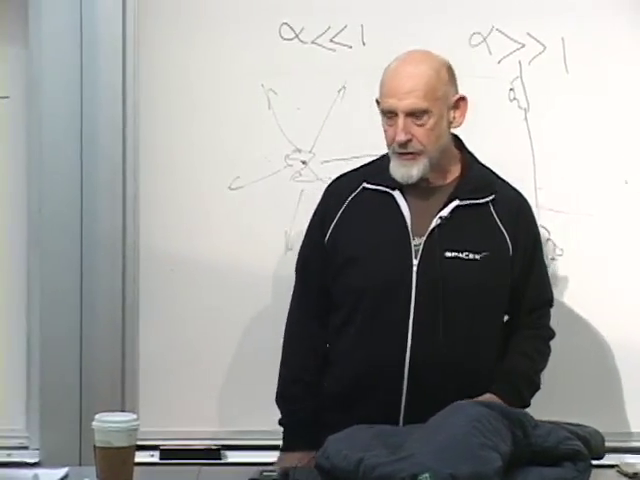
\includegraphics[width=0.72\textwidth]{lecture_01_figure_02.png}
\lectureframe{00:38:22.500}

\vspace{1em}

\begin{tikzpicture}[scale=0.95]
\draw (-5.3,-2.4) rectangle (-1.0,2.1);
\draw (0.3,-2.4) rectangle (4.6,2.1);

\node at (-3.15,2.55) {$\alpha \ll 1$};
\node at (2.45,2.55) {$\alpha \gg 1$};

\draw[line width=0.9pt] (-3.15,-0.15) circle (0.22);
\draw[->,line width=0.8pt] (-3.15,0.07) -- (-3.15,1.35);
\draw[->,line width=0.8pt] (-2.98,-0.01) -- (-1.95,1.00);
\draw[->,line width=0.8pt] (-3.32,-0.01) -- (-4.35,1.00);
\draw[->,line width=0.8pt] (-2.95,-0.23) -- (-1.80,-0.95);
\draw[->,line width=0.8pt] (-3.35,-0.23) -- (-4.50,-0.95);

\draw[line width=1.0pt] (2.15,-1.8) .. controls (1.95,-0.6) and (1.95,0.8) .. (2.15,1.55);
\draw[line width=1.0pt] (2.75,-1.8) .. controls (2.95,-0.6) and (2.95,0.8) .. (2.75,1.55);
\draw[line width=0.8pt] (2.15,-0.85) -- (2.75,-0.85);
\draw[line width=0.8pt] (2.45,1.55) -- (2.45,1.95);
\end{tikzpicture}
\caption{Comparación entre acoplamiento débil--fuerte en la electrodinámica cuántica, durante la discusión de la energía de interacción. El diagrama aísla los dos regímenes que Susskind presenta: una nube tenue con acoplamiento débil y otra que se multiplica con acoplamiento fuerte.}
\end{figure}

La razón por la que esta figura aparece aquí, aunque la comparación entre acoplamiento débil--y fuerte se introdujo antes, es que en la lección Susskind vuelve a dibujar el contraste más adelante, al responder preguntas sobre la energía de interacción y la estructura que se multiplica.

\section{Teorías de branas pares y dimensión adicional emergente}

Hasta aquí, la lección ha desarrollado con fuerza la idea del intercambio: fermión frente a bosón, electrón frente a monopolo, cuerda F frente a cuerda D. El paso siguiente es más sorprendente. Susskind pasa a otra versión de la teoría de cuerdas, con D-branas de dimensión par en lugar de impar. La distinción importa porque en esta teoría no hay una cuerda D que intercambiar con la cuerda F. Hay D0-branas, D2-branas, D4-branas y así sucesivamente.

Por tanto, el límite de acoplamiento fuerte no puede consistir simplemente en cambiarle el nombre a una cuerda por el de otra. Según la lección, ocurre algo más extraño: se hace manifiesta una dimensión espacial adicional. Susskind lo enuncia deliberadamente primero de la forma más dramática --- ``aparece una nueva dimensión'' --- y enseguida lo reformula con más cuidado: una dirección compacta muy pequeña se expande hasta que ya no se puede ignorar.

El recuento forma parte de la idea, así que se detiene a examinarlo:
\begin{equation}
\begin{aligned}
10\text{-dimensional string theory} &= 9\text{ space}+1\text{ time},\\
11\text{-dimensional theory} &= 10\text{ space}+1\text{ time}.
\end{aligned}
\end{equation}
La afirmación de la lección es que el límite de acoplamiento fuerte de la teoría de branas pares es efectivamente undimensional.

\editorialnote{La teoría de branas pares es la teoría de cuerdas de tipo IIA, y su compleción a acoplamiento fuerte es la teoría M. En unidades estándar, el radio del círculo emergente y la longitud de Planck undimensional escalan como \(R_{11}=g_s\ell_s\) y \(\ell_{11}=g_s^{1/3}\ell_s\). Estos nombres y fórmulas hacen explícito el diccionario moderno que subyace a la descripción geométrica de la lección.}

\subsection{El sándwich de mantequilla de cacahuete}

Para imaginar la dirección compacta, Susskind usa el modelo del ``sándwich de mantequilla de cacahuete'': dos láminas de pan infinitamente delgadas, con espacio real entre ellas. La regla especial es que al salir por un lado se vuelve por el otro. En una notación convencional que la lección describe de forma pictórica, no formal, se puede escribir
\begin{equation}
y \sim y + 2\pi R.
\end{equation}
Si \(R\) es muy pequeño, los observadores que viven en el sándwich describen efectivamente su mundo como de menor dimensión. Entonces, el cambio clave a acoplamiento fuerte es
\begin{equation}
g\uparrow
\qquad \Longrightarrow \qquad
R_{\mathrm{compact}}\uparrow.
\end{equation}
Eso es lo que quiere decir Susskind cuando afirma que aparece una nueva dimensión espacial: no que el espacio se cree de la nada, sino que una dirección compacta antes diminuta se expande y se vuelve visible en la teoría efectiva.

\begin{figure}[htbp]
\centering
\resizebox{\linewidth}{!}{%
\begin{tikzpicture}[scale=0.95]
\draw[line width=0.9pt] (-5,1.7) -- (5,1.7);
\draw[line width=0.9pt] (-5,-1.7) -- (5,-1.7);

\node[left] at (-5,1.7) {ceiling};
\node[left] at (-5,-1.7) {floor};

\draw[->,line width=0.8pt] (5.2,1.45) -- (5.2,-1.45);
\draw[->,line width=0.8pt] (5.5,-1.45) -- (5.5,1.45);
\node[right] at (5.55,0) {periodic};

\draw[line width=1.0pt] (-2.6,0.45) -- (2.2,0.45);
\draw[line width=1.0pt] (-2.6,-0.05) -- (2.2,-0.05);
\draw[line width=1.0pt] (-2.6,0.45) -- (-2.6,-0.05);
\draw[line width=1.0pt] (2.2,0.45) -- (2.2,-0.05);
\node at (-0.2,0.9) {floating D2-brane};

\draw[line width=1.0pt] (3.15,-1.7) -- (3.8,-1.7);
\draw[line width=1.0pt] (3.15,1.7) -- (3.8,1.7);
\draw[line width=1.0pt] (3.15,-1.7) -- (3.15,1.7);
\draw[line width=1.0pt] (3.8,-1.7) -- (3.8,1.7);
\node[right] at (3.95,0) {D2 ribbon};

\fill (-3.8,0) circle (0.07);
\node[below] at (-3.8,-0.05) {D0};
\end{tikzpicture}
}%
\caption{La compactificación en forma de sándwich. Los bordes superior e inferior están identificados periódicamente; una D2-brana flota entre ellos como una alfombra, mientras que otra se extiende del suelo al techo y parece una cuerda cuando la dirección compacta es pequeña.}
\end{figure}

\subsection{¿Qué ocurre con las D0- y las D2-branas?}

La lección pregunta ahora qué ocurre con las D0-branas y las cuerdas. La respuesta no es simétrica. A medida que \(g\) aumenta, las D0-branas se vuelven cada vez más ligeras; en la interpretación de dimensión superior, se incorporan a la torre de partículas que llevan momento en la dirección recién manifiesta. Así, un objeto pesado y complejo en la descripción de acoplamiento débil se convierte en una excitación ligera ordinaria en la descripción de acoplamiento fuerte.

La relación entre las masas muestra la identificación:
\begin{equation}
M_{D0}(n)=\frac{n}{g_s\ell_s}
=\frac{n}{R_{11}}
=M_{\mathrm{KK}}(n).
\end{equation}
\editorialnote{Susskind llama a las D0-branas ``los gravitones'' de la teoría undimensional. Más precisamente, sus estados ligados son los modos de momento de Kaluza--Klein del multiplete de supergravedad undimensional, cuyo sector sin masa contiene el gravitón. Esta distinción conserva la identificación física de la lección y evita afirmar literalmente que se trata de una sola partícula.}

Las D2-branas explican el destino de las cuerdas. En la lección se destacan dos configuraciones:
\begin{enumerate}
\item una D2-brana que flota entre el suelo y el techo, como una alfombra en la mantequilla de cacahuete;
\item una D2-brana que se extiende del suelo al techo como una cinta, extendida a lo largo de la dirección visible.
\end{enumerate}
Cuando el sándwich es delgado, la cinta parece efectivamente unidimensional. Es el objeto que los observadores de baja energía llaman cuerda. A medida que se abre la dirección compacta, ese mismo objeto se vuelve inequívocamente parecido a una membrana. Como ahora ocupa más espacio en la dirección vertical, se vuelve pesado y deja de parecer una cuerda.

\paragraph{La lógica de la transición.}
\begin{enumerate}
\item Partimos de una dirección compacta muy pequeña, de modo que la cinta que va del suelo al techo se comporta, en la práctica, como una cuerda.
\item Aumentamos \(g\) y la dirección compacta se expande.
\item Las D0-branas se vuelven ligeras y se reinterpretan como estados de momento de Kaluza--Klein en la teoría de dimensiones superiores.
\item La cinta de D2-brana, que parecía una cuerda, se convierte en una membrana visiblemente extendida y se vuelve pesada.
\end{enumerate}
Este es el punto de inflexión de la lección: de la dualidad a la geometría emergente. El acoplamiento fuerte no se limita a intercambiar un objeto por otro; cambia cuál es la geometría más conveniente para describir el sistema.

Susskind se detiene en lo extraño que suena todo esto. La red de identificaciones propuestas exigía difíciles relaciones de consistencia matemática; algunas de ellas primero se presentaron a los físicos como conjeturas y luego fueron demostradas por matemáticos. No afirma que se conozca cada vacío realista de la teoría de cuerdas, sino que la propia red de dualidades ha superado pruebas de rigor inusualmente exigente.

Si el acoplamiento varía de un lugar a otro en este marco idealizado, la geometría más conveniente también puede variar. Una región puede parecer casi de diez dimensiones, con cuerdas ligeras y D0-branas pesadas; otra puede abrirse a la descripción de once dimensiones, con membranas enrolladas pesadas y modos de Kaluza--Klein ligeros. El cambio local de lenguaje forma parte de la misma red de dualidades.

La transcripción recoge brevemente el nombre de estas relaciones como ``desigualdades.'' Por el contexto, la palabra que se quería decir es \emph{dualidades}: relaciones entre extremos opuestos del espacio de parámetros. La corrección importa porque la conclusión de la lección es precisamente que no se conoce una lista única de constituyentes fundamentales. Las cuerdas, las branas, las partículas y la geometría de dimensiones superiores pueden transformarse unas en otras; o bien ningún elemento de la red es absolutamente fundamental, o bien existe una organización más profunda que aún se desconoce.

\section{D3-branas, membranas enrolladas y una imagen geométrica de la dualidad}

Tras la pausa, Susskind describe explícitamente el tema como una ``enorme red'' de teorías e ideas interconectadas. Los siguientes ejemplos no son nuevos efectos aislados, sino puentes que enlazan los anteriores.

\subsection{La variedad de mundo de una D3-brana}

El primer puente se construye con una D3-brana. Una D3-brana tiene tres dimensiones espaciales, y un observador confinado en ella podría confundirla fácilmente con el espacio ordinario. La brana puede curvarse y fluctuar, mientras que las cuerdas que terminan en ella pueden unirse, dividirse y dispersarse. Para un observador que solo ve las direcciones a lo largo de la brana, cada extremo parece una partícula, y las interacciones entre los extremos, una teoría cuántica de campos ordinaria.

\begin{figure}[htbp]
\centering
\resizebox{\linewidth}{!}{%
\begin{tikzpicture}[scale=1.0]
\draw[fill=gray!15] (-4,-0.35) rectangle (4,0.35);
\node at (0,-0.75) {D3-brane};

\draw[line width=0.9pt] (-1.5,2.1) -- (-1.5,0.35);
\fill (-1.5,0.35) circle (0.07);
\node[left] at (-1.72,1.25) {F-string};
\node[below left] at (-1.5,0.32) {electric charge};

\draw[line width=1.5pt] (1.7,2.1) -- (1.7,0.35);
\fill (1.7,0.35) circle (0.09);
\node[right] at (1.95,1.25) {D-string};
\node[below right] at (1.7,0.32) {magnetic monopole};
\end{tikzpicture}
}%
\caption{Interpretación en términos de la variedad de mundo de una D3-brana. El extremo de una cuerda F aparece como una carga eléctrica; el extremo de una cuerda D, como un monopolo magnético.}
\end{figure}

Esta es una de las identificaciones más satisfactorias de la lección. Para un observador en la variedad de mundo, una cuerda F que termina en la D3-brana aparece como una carga eléctrica. Una cuerda D que termina en esa misma brana aparece como un monopolo magnético. En otras palabras, la dualidad entre las cuerdas F y D se convierte, en la variedad de mundo de la D3-brana, en la dualidad eléctrica--magnética de la teoría de campos ordinaria. Lo que antes era una analogía ahora es un diccionario explícito.

\editorialnote{Para una pila de D3-branas, la descripción de baja energía en el volumen de mundo es la teoría de Yang--Mills supersimétrica en cuatro dimensiones \(\mathcal N=4\). Su dualidad eléctrica--magnética es la realización en teoría de campos de la S-dualidad de la teoría de tipo IIB; una sola brana da el límite abeliano que se usa de forma pictórica en la clase.}

\subsection{Dos direcciones compactas y enrollamientos asimétricos}

Susskind vuelve entonces a la geometría de dimensiones superiores y compactifica no una, sino dos direcciones pequeñas. Como no se pueden dibujar once dimensiones en una pizarra, comprime en una sola dirección horizontal visible las siete direcciones grandes que no aparecen en el esquema y dibuja explícitamente las dos compactas. Insiste en representar la compactificación de forma asimétrica, porque una dirección compacta debe ser más corta que la otra para que las cuerdas efectivas tengan tensiones distintas.

\begin{figure}[htbp]
\centering
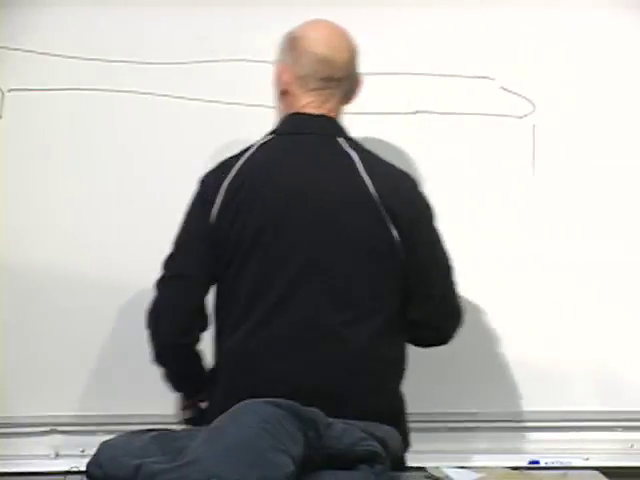
\includegraphics[width=0.78\textwidth]{lecture_01_figure_03.png}
\lectureframe{01:10:25.000}
\caption{Configuración final en la pizarra para las dos membranas enrolladas. Los ciclos compactos corto y largo producen las cintas similares a cuerdas F y D dibujadas a la derecha.}
\end{figure}

Una membrana puede enrollarse alrededor de cualquiera de las dos direcciones compactas y parecer una cuerda desde las direcciones no compactas. Si \(R_1\) y \(R_2\) son los radios de los dos círculos, sus tensiones efectivas son
\begin{equation}
\begin{aligned}
T_{(1)}&=2\pi R_1 T_{\mathrm{M2}},\\
T_{(2)}&=2\pi R_2 T_{\mathrm{M2}},\\
\frac{T_{(1)}}{T_{(2)}}&=\frac{R_1}{R_2}.
\end{aligned}
\end{equation}
Así, tamaños distintos de los círculos producen tensiones distintas para las cuerdas. Si identificamos el enrollamiento más corto con la cuerda F ligera y el más largo con la cuerda D pesada, podemos escribir esquemáticamente
\begin{equation}
g_s\sim \frac{R_{\mathrm{short}}}{R_{\mathrm{long}}},
\qquad
\frac{T_{\mathrm{D1}}}{T_{\mathrm{F1}}}\sim \frac{1}{g_s}.
\end{equation}

\begin{classroomqa}
\audiencequestion{¿Puede entenderse el acoplamiento de esta imagen como la razón entre las dos dimensiones compactas? \lecturetimestamp{01:10:13}}
\lecturerresponse{Sí. El parámetro de acoplamiento débil--fuerte se expresa geométricamente como una razón de aspecto. Si se hace corta una dirección, el acoplamiento se vuelve pequeño; intercambiar las dos direcciones intercambia las cuerdas ligera y pesada.}
\end{classroomqa}

\editorialnote{En la lección se llama provisionalmente \(\alpha\) a esta razón, reutilizando el símbolo que antes se había usado para la constante de estructura fina de la electrodinámica cuántica. Aquí escribimos \(g_s\) para mantener separados ambos significados. En la construcción completa de la teoría M, el acoplamiento de tipo IIB está codificado en la estructura compleja del toro compacto de dos dimensiones; el numerador preciso depende de cómo se etiqueten sus ciclos.}

La imagen de la membrana enrollada puede resumirse sin la distorsión de perspectiva del dibujo en la pizarra:

\begin{figure}[htbp]
\centering
\begin{tikzpicture}[scale=1.0]
\draw[line width=0.9pt] (0,0) rectangle (5.2,2.2);
\node[below] at (2.6,-0.2) {\(R_1\)};
\node[right] at (5.4,1.1) {\(R_2\)};

\draw[->,line width=0.7pt] (5.45,1.9) -- (5.45,0.3);
\draw[->,line width=0.7pt] (5.7,0.3) -- (5.7,1.9);
\draw[->,line width=0.7pt] (0.4,-0.35) -- (4.8,-0.35);
\draw[->,line width=0.7pt] (4.8,-0.6) -- (0.4,-0.6);

\draw[line width=1.0pt] (1.1,0) -- (1.6,0) -- (1.6,2.2) -- (1.1,2.2) -- cycle;
\node at (1.35,2.55) {light};

\draw[line width=1.0pt] (0,1.45) -- (5.2,1.45);
\draw[line width=1.0pt] (0,1.00) -- (5.2,1.00);
\node at (4.55,1.95) {heavy};

\node at (1.35,-0.95) {F-string};
\node at (4.55,0.55) {D-string};
\end{tikzpicture}
\caption{Desde las direcciones no compactas, ambas configuraciones de membrana enrollada parecen cuerdas; sin embargo, las distintas escalas compactas hacen que una cuerda efectiva sea más ligera que la otra.}
\end{figure}

Esta es la versión geométrica de la historia de dualidad anterior. Al comprimir una dirección y estirar la otra, un objeto enrollado se vuelve más pesado y el otro más ligero, de modo que las funciones de las cuerdas F y D pueden intercambiarse.

\begin{classroomqa}
\audiencequestion{Si las direcciones compactas son cíclicas, ¿los objetos enrollados tienen anchura infinita? \lecturetimestamp{01:10:41}}
\lecturerresponse{No. Un círculo compacto tiene una circunferencia finita, aunque se pueda recorrer repetidamente sin llegar a un borde. La parte superior y la inferior del dibujo abierto en la pizarra representan el mismo punto, igual que los extremos de un intervalo pueden representar un mismo punto del círculo.}
\end{classroomqa}

\begin{figure}[htbp]
\centering
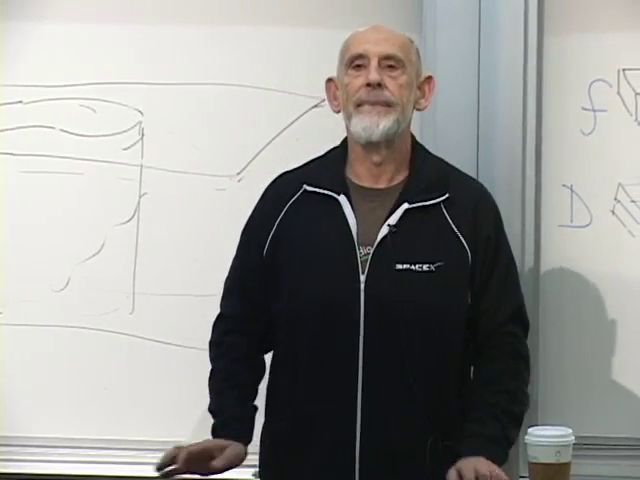
\includegraphics[width=0.78\textwidth]{lecture_01_figure_04.png}
\lectureframe{01:12:25.000}

\vspace{1em}

\begin{tikzpicture}[scale=0.95]
\draw[line width=0.9pt,->] (-3.7,0) arc[start angle=180,end angle=535,radius=0.95];
\node at (-2.75,0) {compact circle};
\draw[line width=0.9pt] (0.0,0) -- (4.8,0);
\fill (0.0,0) circle (0.06);
\fill (4.8,0) circle (0.06);
\draw[<->] (0.0,-0.45) -- (4.8,-0.45);
\node at (2.4,-0.75) {cut-open interval of length \(2\pi R\)};
\node[above] at (0.0,0.1) {same point};
\node[above] at (4.8,0.1) {same point};
\end{tikzpicture}
\caption{Un círculo compacto y su representación abierta en la pizarra. Al cruzar un extremo se vuelve a aparecer por el otro; en cambio, al avanzar en una dirección no compacta mientras se recorre el círculo se trazaría una hélice.}
\end{figure}

\begin{classroomqa}
\audiencequestion{¿Por qué la trayectoria compacta es un círculo y no una hélice? \lecturetimestamp{01:12:23}}
\lecturerresponse{En cada punto fijo de la dirección no compacta, la dirección compacta es un círculo. Solo aparece una hélice si se avanza en la dirección no compacta mientras se dan vueltas alrededor del círculo. El intervalo dibujado en la pizarra no es más que un círculo abierto por un corte, con sus dos extremos identificados.}
\end{classroomqa}

\begin{classroomqa}
\audiencequestion{¿Explica esta geometría por sí sola cómo una D-brana puede parecer un conjunto de cuerdas F cuando se la examina de cerca? \lecturetimestamp{01:12:49}}
\lecturerresponse{La conexión existe, pero no resulta evidente en esta imagen elemental; para verla hace falta un aparato geométrico más avanzado. El diagrama sirve para organizar la dualidad, no para derivar cada descripción de sus constituyentes microscópicos.}
\end{classroomqa}

\begin{classroomqa}
\audiencequestion{¿Podrían intercambiarse las direcciones compactas larga y corta al desplazarse por el espacio o con el paso del tiempo? \lecturetimestamp{01:13:35}}
\lecturerresponse{Cualquiera de las dos posibilidades se da en el modelo idealizado. Al aplastar un ciclo y expandir el otro, se intercambia cuál de las cuerdas enrolladas es ligera. Esta es otra razón por la que ``cuerda fundamental'' es solo un nombre: la descripción más conveniente puede cambiar de una región a otra o con el tiempo.}
\end{classroomqa}

\section{Idealización, puntos de simetría especial y el paisaje}

En el último tramo de la lección, Susskind se aleja de los elegantes ejemplos de dualidad y se pregunta qué nos dicen, y qué no, sobre el mundo real.

Primero, Susskind advierte que las dualidades que se pueden controlar con precisión son características de teorías supersimétricas muy idealizadas, en las que los bosones y los fermiones tienen masas exactamente iguales. Su analogía son las órbitas circulares de la mecánica newtoniana: se estudian primero porque son simétricas y matemáticamente manejables, no porque el movimiento real de los planetas se limite a círculos perfectos. Del mismo modo, las teorías de cuerdas supersimétricas son más fáciles de analizar porque son más simétricas que lo que parece ser la naturaleza.

Aun así, la idealización aporta información. Una órbita circular perfecta no representa un sistema planetario realista, pero muestra características que también se dan en órbitas menos simétricas. De modo parecido, los ejemplos supersimétricos muestran formas coherentes de compatibilizar la mecánica cuántica, la gravedad y la estructura microscópica. La formulación deliberadamente tajante de Susskind es que las teorías de cuerdas manejables no son, literalmente, la teoría de nuestro mundo; su valor reside en revelar fenómenos que probablemente también aparezcan en contextos menos simétricos y más difíciles de tratar.

\subsection{Un conjunto de piezas con muchos resultados posibles}

Las D-branas son solo parte del conjunto de piezas disponible. La lección también menciona flujos, orbifolds y orientifolds. Primero se elige una geometría compacta y luego qué branas y flujos ocupan sus ciclos. Incluso el sencillo sándwich cambia su física de dimensiones inferiores cuando se introduce una D2-brana flotante, dos o tres. Añadir o quitar estos elementos cambia las partículas, las interacciones y los parámetros efectivos.

Supongamos, siguiendo el recuento esquemático de la lección, que un espacio compacto de seis dimensiones tiene aproximadamente \(500\) ciclos y que en cada ciclo se puede elegir entre unas \(10\) configuraciones de branas enrolladas, flujos o estructuras relacionadas. Entonces, el número de construcciones crece como
\begin{equation}
N_{\mathrm{vacua}} \sim 10^{500}.
\end{equation}
La lógica del recuento de la lección es elemental:
\begin{equation}
10 \times 10 \times \cdots \times 10 = 10^{500}
\end{equation}
con \(500\) factores. La analogía con el ADN expresa la misma idea en términos más familiares:
\begin{equation}
N_{\mathrm{DNA}}(500)=4^{500}.
\end{equation}
Durante la comparación con el ADN, alguien del público comprueba que hay cuatro alternativas a lo largo de una hebra: A, C, G y T. La corrección refuerza el argumento, no lo cambia. Una lista corta de opciones locales, repetida muchas veces, produce una cantidad enorme de configuraciones globales. El exponente preciso no es lo importante, y Susskind califica \(10^{500}\) de una estimación demasiado baja, ya anticuada; lo importante es la proliferación combinatoria.

Así se completa la inversión de la expectativa reduccionista inicial. Una física de partículas complicada no tiene por qué surgir de reglas microscópicas complicadas. Puede surgir porque nuestro vacío es una configuración compleja de muchos elementos sencillos, igual que un organismo complejo puede codificarse mediante una secuencia construida a partir de cuatro bases.

\begin{classroomqa}
\audiencequestion{Una vez identificadas las descripciones equivalentes relacionadas por dualidad, ¿la información completa seleccionaría solo uno o unos pocos de estos vacíos posibles como descripciones de nuestro mundo? \lecturetimestamp{01:26:11}}
\lecturerresponse{Es de suponer que seleccionaría un conjunto restringido, pero muchos vacíos distintos podrían parecer extremadamente similares a las energías accesibles. El número citado para el paisaje pretende seguir siendo grande incluso tras identificar las descripciones duales, y los detalles irrelevantes de alta energía pueden funcionar como el ``ADN basura.''}
\end{classroomqa}

\subsection{Puntos simétricos y complejidad genérica}

Dentro del paisaje hay puntos con simetrías especiales. En la imagen geométrica, una configuración con razones de aspecto iguales,
\begin{equation}
R_1=R_2,
\end{equation}
hace que las dos descripciones del objeto enrollado sean igual de sencillas. En la analogía eléctrica--magnética, esto se representa esquemáticamente mediante
\begin{equation}
m_{\mathrm{monopole}}=m_e.
\end{equation}

\begin{figure}[htbp]
\centering
\begin{tikzpicture}[scale=0.95]
\draw[line width=0.9pt] (-4.5,-1.0) rectangle (-2.5,1.0);
\draw[<->] (-4.5,-1.35) -- (-2.5,-1.35);
\draw[<->] (-2.15,-1.0) -- (-2.15,1.0);
\node at (-3.5,1.45) {symmetric point};
\node at (-3.5,-1.75) {$R_1=R_2$};

\draw[line width=0.9pt] (0.0,-0.55) rectangle (4.8,0.55);
\draw[<->] (0.0,-0.9) -- (4.8,-0.9);
\draw[<->] (5.15,-0.55) -- (5.15,0.55);
\node at (2.4,1.45) {lopsided point};
\node at (2.4,-1.3) {$R_1\ne R_2$};
\end{tikzpicture}
\caption{Una compactificación con razones de aspecto iguales trata simétricamente las dos cuerdas enrolladas; una compactificación desequilibrada hace que una de las descripciones sea mucho más ligera que la otra.}
\end{figure}

\begin{classroomqa}
\audiencequestion{¿Hay vacíos en el paisaje donde la construcción sea mucho más sencilla porque las descripciones con cuerdas F y D coinciden? \lecturetimestamp{01:27:21}}
\lecturerresponse{Sí, hay puntos con simetrías especiales. Nuestro mundo no parece estar en uno de ellos: la partícula eléctrica conocida y un monopolo magnético no tienen la misma masa. Se desconoce por qué la naturaleza ocupa un punto desequilibrado.}
\end{classroomqa}

\editorialnote{La igualdad entre la masa del electrón y la del--monopolo es una característica esquemática de un modelo autodual adecuadamente protegido, no una predicción de la electrodinámica cuántica ordinaria sin supersimetría. Expresa la idea de punto de simetría de la lección, no una afirmación sobre el electrón observado.}

Susskind recuerda entonces una analogía de la teoría de la comunicación. Los códigos aleatorios pueden ser extraordinariamente buenos, mientras que los más fáciles de describir y decodificar tienen estructura matemática adicional y, históricamente, dieron peores resultados. Más adelante, la teoría de códigos encontró construcciones estructuradas muy eficaces, pero la analogía sigue en pie: todo lo que se puede nombrar o describir de manera concisa ocupa una región muy especial y de baja complejidad dentro del espacio completo de posibilidades. Del mismo modo, los vacíos de cuerdas más fáciles de calcular pueden ser atípicamente sencillos.

Por tanto, quizá convenga plantear otras preguntas. En lugar de exigir una descripción exacta de cada detalle microscópico de la compactificación, se puede preguntar qué características son comunes o genéricas en un conjunto amplio de posibilidades. Susskind presenta esto como un problema de investigación, no como una conclusión establecida, y rechaza los argumentos ideológicos como sustituto del cálculo.

\subsection{Cuestiones cosmológicas}

\begin{classroomqa}
\audiencequestion{¿Una dirección compacta de circunferencia enorme se distingue observacionalmente de una dirección infinita? ¿Y sabemos que nuestras tres grandes dimensiones espaciales son infinitas? \lecturetimestamp{01:30:03}}
\lecturerresponse{No sabemos si son infinitas. Una tres-esfera cerrada puede expandirse sin dejar de ser compacta. Las mediciones de una curvatura casi nula solo dan un límite inferior para el radio de curvatura, igual que medir un terreno casi llano puede acotar el tamaño de la Tierra sin demostrar que su superficie sea infinita. Solo detectar una curvatura o una identificación global permitiría determinar la escala finita.}
\end{classroomqa}

\begin{classroomqa}
\audiencequestion{Si el acoplamiento puede variar en el espacio en el modelo idealizado, ¿cómo podría producirse esa variación en el mundo real? \lecturetimestamp{01:32:43}}
\lecturerresponse{No como la variación suave sin restricciones del ejemplo simétrico. La posibilidad realista que se analizará más adelante es una variación mediante transiciones discretas entre regiones con leyes efectivas distintas. Que se produzcan tales saltos es una cuestión cosmológica.}
\end{classroomqa}

\editorialnote{Esta respuesta debe entenderse como un anticipo de la lección sobre vacíos de flujo y transiciones entre dominios, no como un teorema general que prohíba todo campo escalar con variación suave. Las observaciones restringen fuertemente las variaciones de los acoplamientos adimensionales, mientras que los mecanismos de estabilización determinan si quedan moduli continuos disponibles en un modelo dado.}

La grabación no conserva la última pregunta del público. La respuesta que sí se conserva dice que el fenómeno propuesto puede darse en algunos tipos de agujeros negros, pero no en el horizonte de un agujero negro ordinario de Schwarzschild, que para un observador en caída libre es localmente un lugar corriente. Como no se puede reconstruir la pregunta con fiabilidad, no se atribuye al intercambio ninguna afirmación más específica.

\section{De los ladrillos a una red de descripciones}

La esperanza de que las capas más profundas de la física deban ser más sencillas ha resultado frágil. En la bosonización en \(1+1\) dimensiones, una misma teoría puede organizarse en torno a fermiones o a bosones, y el fermión reaparece como un kink. En la electrodinámica cuántica, el acoplamiento débil y el fuerte intercambian las funciones descriptivas del electrón y el monopolo magnético. En la teoría de cuerdas, las cuerdas F y D reproducen el mismo patrón, y en la teoría de branas pares el acoplamiento fuerte lleva aún más lejos esta idea: se expande una dirección compacta, las D0-branas se convierten en estados de momento de Kaluza--Klein y las cuerdas efectivas se reinterpretan como membranas enrolladas en una geometría de dimensiones superiores. Por tanto, la teoría cuántica de campos y la teoría de cuerdas modernas no ofrecen una respuesta única y definitiva a la pregunta ``¿cuáles son los ladrillos y cuáles las casas?'' Ofrecen una red de descripciones, cada una eficiente en su propio régimen, junto con un vasto paisaje de construcciones posibles cuyo resultado genérico es la complejidad, no la simplicidad.

\chapter{Geometría, información y ley del área de los agujeros negros}

\lectureoverview{El destino anunciado es la cosmología, pero el camino más corto empieza volviendo a la relatividad especial. Una métrica nos indica la geometría del espacio-tiempo, y la condición de tiempo propio nulo nos dice cómo se propaga la luz. Llevaremos esa regla a la geometría de Schwarzschild, distinguiremos el horizonte de la singularidad y luego preguntaremos qué ocurre con la información cuando un agujero negro se evapora. La respuesta empieza con la entropía ordinaria y termina con el argumento de Bekenstein basado en un bit: un agujero negro almacena información en unidades de área del horizonte, no de volumen.}

Susskind aplaza brevemente el balance prometido de los éxitos y fracasos de la teoría de cuerdas. Dice que es tarde y que resulta más útil abordar el contenido que hacer un balance. El contenido de esta noche es la geometría y la termodinámica mínimas necesarias para plantear el problema de la información de los agujeros negros.

\section{Una regla para la luz}

La relatividad especial trata el espacio y el tiempo como un único objeto geométrico. Para sucesos próximos separados por \(dt,dx,dy,dz\), Susskind adopta la convención de signos mayormente negativa y escribe
\begin{equation}
d\tau^2=dt^2-\frac{1}{c^2}\left(dx^2+dy^2+dz^2\right).
\end{equation}
Los signos opuestos de las partes temporal y espacial distinguen la geometría de Minkowski de la geometría euclidiana cuatridimensional. El factor \(1/c^2\) solo permite compatibilizar las unidades; si medimos el tiempo y la distancia de manera compatible, podemos fijar \(c=1\).

Para una separación temporal \(d\tau^2>0\), y \(d\tau\) es el tiempo propio registrado por un reloj que sigue la trayectoria. En cambio, las separaciones espaciales cumplen \(d\tau^2<0\). El caso que necesitamos esta noche está justo entre ambas. Un rayo de luz sigue una trayectoria \emph{nula},
\begin{equation}
d\tau^2=0.
\end{equation}
Si restringimos primero el movimiento al eje \(x\), obtenemos
\begin{align}
0&=dt^2-\frac{dx^2}{c^2},\\
c\,dt&=\pm dx,\\
\frac{dx}{dt}&=\pm c.
\end{align}
Los signos describen rayos que se propagan hacia la derecha y hacia la izquierda. El valor numérico asignado a \(c\) cambia al sustituir los centímetros por metros o kilómetros; la afirmación invariante no es un número, sino la condición de nulidad.

La relatividad general complica la métrica, pero no esta regla. Con coordenadas \(x^\mu\), \(\mu=0,1,2,3\),
\begin{equation}
ds^2=g_{\mu\nu}(x)\,dx^\mu dx^\nu,
\end{equation}
donde se suman los índices repetidos y los coeficientes pueden variar de un punto a otro. Para hallar las direcciones localmente permitidas para la luz, igualamos a cero esta forma cuadrática.

\section{Coordenadas esféricas y métrica de Schwarzschild}

Un agujero negro no rotatorio tiene simetría esférica, así que las coordenadas cartesianas ocultan la estructura útil. Sea \(r\) la distancia radial y sean \(\theta,\phi\) las coordenadas que indican una dirección sobre una esfera unitaria. Su elemento de línea es
\begin{equation}
d\Omega^2=d\theta^2+\sin^2\theta\,d\phi^2.
\end{equation}
Por tanto, sobre una esfera de radio \(r\), los desplazamientos angulares contribuyen con \(r^2d\Omega^2\). El espacio-tiempo plano en coordenadas esféricas es
\begin{equation}
d\tau^2=dt^2-\left(dr^2+r^2d\Omega^2\right),
\qquad (c=1).
\end{equation}

Susskind no deriva la solución del agujero negro a partir de las ecuaciones de Einstein. La escribe y nos pide que la examinemos. La pizarra hace explícita la comparación que se propone.

\begin{figure}[htbp]
\centering
\includegraphics[width=0.86\textwidth]{lecture_02_figure_02.png}
\caption{El espacio-tiempo esférico plano aparece sobre la deformación de Schwarzschild. Se ven juntos el factor repetido \(1-2GM/(c^2r)=1-R_s/r\) y el esquema radial.}
\lectureframe{00:19:12.520}
\end{figure}

Para un agujero negro de masa \(M\), definimos el radio de Schwarzschild
\begin{equation}
R_s=\frac{2GM}{c^2}.
\end{equation}
El elemento de línea exterior es
\begin{equation}
d\tau^2=\left(1-\frac{R_s}{r}\right)dt^2
-\frac{dr^2/c^2}{1-R_s/r}
-\frac{r^2}{c^2}d\Omega^2.
\label{eq:schwarzschild-explicit-c}
\end{equation}
De forma equivalente, al fijar \(c=1\),
\begin{equation}
ds^2=\left(1-\frac{2GM}{r}\right)dt^2
-\frac{dr^2}{1-2GM/r}-r^2d\Omega^2.
\label{eq:schwarzschild}
\end{equation}
A grandes distancias, \(R_s/r\ll1\), y se recupera la métrica esférica plana. Esta comprobación asintótica importa más que memorizar la fórmula, aunque Susskind recomienda esto último como tema de conversación para fiestas.

\editorialnote{La pizarra alterna entre \(d\tau^2\) y \(ds^2\), y no muestra de forma coherente todos los factores de \(c\). La ecuación~\eqref{eq:schwarzschild-explicit-c} sigue la convención de la coordenada temporal usada en la clase, en la que \(t\) tiene unidades de tiempo. La forma estándar con \(x^0=ct\) es algebraicamente equivalente.}

\subsection{El horizonte no es la singularidad}

Hay dos radios que parecen sospechosos en estas coordenadas. En \(r=R_s=2GM\), usando unidades naturales, el coeficiente de \(dt^2\) se anula y el de \(dr^2\) diverge. En \(r=0\), la propia curvatura se vuelve singular. No se trata de dos versiones del mismo suceso:
\begin{equation}
\begin{aligned}
r=R_s &:\quad \text{horizon},\\
r=0 &:\quad \text{curvature singularity}.
\end{aligned}
\end{equation}

Las fuerzas de marea establecen la distinción física. El campo gravitatorio varía a lo largo de un cuerpo extenso: puede tirar con más fuerza de los pies que de la cabeza, estirando el cuerpo mientras comprime las direcciones transversales. En el horizonte, esas fuerzas de marea son finitas y, en el horizonte de un agujero negro suficientemente masivo, pueden ser muy pequeñas. Allí no tiene por qué ocurrir nada catastrófico a nivel local. En cambio, en \(r=0\) las fuerzas de marea divergen. Los coeficientes alarmantes en \(r=R_s\) indican un defecto de las coordenadas de Schwarzschild; la singularidad en \(r=0\) es física.

\editorialnote{La finitud de la curvatura en \(r=R_s\) puede comprobarse mediante el escalar de Kretschmann \(R_{\mu\nu\rho\sigma}R^{\mu\nu\rho\sigma}=48G^2M^2/(c^4r^6)\), que es finito en el horizonte y solo diverge cuando \(r\to0\). Este invariante no se escribió en la clase, pero precisa la distinción basada en las fuerzas de marea.}

\section{Luz radial cerca del horizonte}

Volvamos ahora a la regla. Un rayo radial mantiene fija su posición angular, de modo que \(d\Omega=0\), y un rayo de luz cumple \(ds^2=0\). En unidades con \(c=1\), la ecuación~\eqref{eq:schwarzschild} da
\begin{equation}
0=\left(1-\frac{2GM}{r}\right)dt^2
-\frac{dr^2}{1-2GM/r}.
\end{equation}
Al multiplicar por \(1-2GM/r\) y extraer la raíz cuadrada, obtenemos dos ramas,
\begin{align}
dr&=\pm\left(1-\frac{2GM}{r}\right)dt,\\
\frac{dr}{dt}&=\pm\left(1-\frac{2GM}{r}\right).
\label{eq:radial-null}
\end{align}
El signo positivo corresponde a la rama saliente y el negativo, a la entrante. A grandes distancias, sus velocidades coordenadas tienden a \(\pm1\). En el horizonte ambas cumplen \(\lvert dr/dt\rvert\to0\): en el tiempo coordenado de Schwarzschild, un rayo saliente parece quedarse allí inmóvil, mientras que un rayo entrante tarda un tiempo coordenado infinito en llegar.

\begin{figure}[htbp]
\centering
\includegraphics[width=0.82\textwidth]{lecture_02_figure_03.png}
\caption{Esquema terminado en la pizarra para las coordenadas \(t\)-\(r\): los rayos nulos radiales se vuelven casi verticales al acercarse al horizonte discontinuo.}
\lectureframe{00:30:25.000}
\end{figure}

\begin{figure}[htbp]
\centering
\begin{tikzpicture}[x=1.0cm,y=0.9cm]
\draw[->] (0,0) -- (6.6,0) node[right] {$r$};
\draw[->] (0,0) -- (0,6.2) node[above] {$t$};
\draw[dashed,thick] (2.0,0) -- (2.0,5.9) node[above] {$r=R_s$};
\draw[thick,->] (2.08,.4) .. controls (2.10,2.2) and (2.55,3.8) .. (5.8,5.7);
\draw[thick,->] (5.8,.5) .. controls (3.2,2.0) and (2.15,4.2) .. (2.03,5.7);
\node[align=center] at (4.7,4.4) {outgoing};
\node[align=center] at (4.5,1.2) {ingoing};
\end{tikzpicture}
\caption{Versión depurada del esquema de la pizarra en tiempo coordenado. La aparente ralentización se refiere a \(t\) de Schwarzschild, no a una incapacidad local de la luz para propagarse a \(c\).}
\end{figure}

Dentro del horizonte, los conos de luz futuros se inclinan tanto hacia dentro que ambas ramas radiales dirigidas al futuro avanzan hacia valores decrecientes de \(r\). Ninguna señal que se origine allí puede escapar al exterior, y toda trayectoria causal futura alcanza la singularidad.

\begin{classroomqa}
\audiencequestion{Si la velocidad de la luz es invariante, ¿qué significa exactamente decir que la luz se ralentiza cerca del horizonte?\lecturetimestamp{00:31:44}}
\lecturerresponse{La cantidad mostrada es \(dr/dt\) en un sistema de coordenadas concreto. La velocidad numérica ya cambia al sustituir metros por centímetros; aquí, las calibraciones radial y temporal efectivas varían con la posición. La afirmación universal es que todo rayo de luz sigue una trayectoria nula, \(ds^2=0\).}
\end{classroomqa}
\editorialnote{Un observador local en caída libre mide que la luz en el vacío se propaga a \(c\); la velocidad coordenada de Schwarzschild que se anula en el horizonte no es una magnitud observable localmente.}

\begin{classroomqa}
\audiencequestion{¿Se cumple la misma afirmación sobre la velocidad nula con independencia del medio material por el que se propaga la luz?\lecturetimestamp{00:33:24}}
\lecturerresponse{No. El reconocimiento disponible no conserva una explicación más extensa de esta respuesta.}
\end{classroomqa}
\editorialnote{La afirmación sobre la velocidad nula se refiere a la propagación en el espacio-tiempo vacío. Las interacciones con la materia pueden dar a un paquete de ondas una velocidad efectiva menor; eso es una propiedad del medio, no un cambio en la velocidad causal local \(c\).}

\begin{classroomqa}
\audiencequestion{¿Cómo se ve un rayo de luz entrante en el mismo diagrama \(t\)-\(r\)?\lecturetimestamp{00:33:32}}
\lecturerresponse{Es la rama que parece recorrer el camino inverso: desde valores grandes de \(r\) se curva hacia el horizonte y se aproxima a él asintóticamente. Tarda un tiempo coordenado infinito \(t\) en llegar.}
\end{classroomqa}
\editorialnote{Un observador en caída libre alcanza y cruza el horizonte en un tiempo propio finito; solo diverge \(t\) de Schwarzschild.}

\section{Por qué la evaporación plantea un problema}

El horizonte merece estudiarse mucho más: cómo se forma, qué ve un observador en caída libre y si ocurre allí algo inusual a nivel local. Susskind aplaza esas preguntas y pasa a la mecánica cuántica. Desde el exterior, la materia y toda la información que la distingue quedan cada vez más comprimidas cerca del horizonte y dejan de estar disponibles. Eso por sí solo no tiene por qué destruir la información; quizá solo la oculte.

El resultado de Hawking vuelve apremiante la cuestión. Desde el punto de vista clásico, un agujero negro en equilibrio parece el objeto más anodino imaginable: esférico, oscuro e incapaz de enviar un mensaje. Pero ``negro'' tiene dos sentidos. Puede significar que no emite nada o que emite radiación térmica de cuerpo negro. Un agujero negro cuántico es negro en el segundo sentido. Tiene temperatura, brilla y pierde energía. Como
\begin{equation}
E=Mc^2,
\qquad
R_s=\frac{2GM}{c^2},
\end{equation}
la radiación reduce tanto su masa como el radio de su horizonte. Si la evaporación acaba eliminando el agujero, ¿qué ocurre con la información que parecía permanecer en el horizonte? Podría destruirse, quedar atrapada en un remanente diminuto o codificarse en la radiación saliente. La tensión entre esas posibilidades constituye el problema de la información, y más adelante la teoría de cuerdas ayudará a precisar su resolución.

Esta noche no se intenta calcular campos cuánticos en el espacio-tiempo curvo. En su lugar, Susskind sigue el camino más sencillo de Bekenstein: primero entender la entropía como información y luego calcular cuánta información puede ocultar un agujero negro.

\section{Información presente pero oculta}

Imaginemos que dividimos una caja en celdas lo bastante pequeñas como para que cada una esté ocupada o vacía. Una cadena binaria---una respuesta por celda---distingue esa configuración de cualquier otra configuración permitida. Para describir materia más realista hay que preguntar por las especies de partículas y otros grados de libertad, pero el principio no cambia: la información se mide por el número mínimo de respuestas afirmativas--negativas necesarias para especificar el estado.

\begin{classroomqa}
\audiencequestion{¿Es esto solo una descripción de un sistema estático?\lecturetimestamp{00:45:49}}
\lecturerresponse{Es una descripción instantánea, correspondiente a un momento dado. La dinámica lleva después ese estado a otro estado.}
\end{classroomqa}

El siguiente principio es más profundo: la evolución de un sistema cerrado no fusiona dos estados microscópicos distintos en uno solo. Si dos configuraciones difieren ahora, sus configuraciones evolucionadas siguen siendo distinguibles en principio. La evolución hamiltoniana clásica es invertible y la evolución cuántica es unitaria.\editorialnote{Las ecuaciones efectivas disipativas solo pueden borrar distinciones porque se han omitido grados de libertad ambientales no observados; el estado completo del sistema cerrado las conserva.}

La bañera hace concreta la diferencia entre pérdida e inaccesibilidad. Dos corrientes de gotas podrían codificar dos textos distintos en código Morse. Cuando el agua se calma, las dos bañeras parecen iguales. Las ondas visibles han desaparecido, pero una medición microscópica completa aún encontraría configuraciones moleculares distintas. El mensaje se ha dispersado entre grados de libertad demasiado pequeños y demasiado numerosos para seguirles la pista.

La entropía es esa información oculta. Respecto de las preguntas macroscópicas que podemos plantear---temperatura, energía total, composición, nivel del agua---siguen siendo posibles muchas distinciones microscópicas, aunque no podamos acceder a ellas. En el lenguaje de la clase, basado en contar bits,
\begin{equation}
S=\hbox{number of hidden bits}.
\end{equation}
La fórmula estadística precisa es \(S=k_B\ln\Omega\), pero para el argumento sobre los agujeros negros basta con la definición cualitativa.

\section{La temperatura como coste de ocultar un bit}

La temperatura es fácil de medir y sorprendentemente indirecta de definir. Susskind toma la entropía y la energía como conceptos primitivos. Supongamos que se restablece un bit de computadora a un valor estándar. El dispositivo físico permanece, pero la computadora pierde la distinción entre sus estados anteriores, cero y uno. Esa distinción no puede desaparecer del mundo completo; se transfiere a grados de libertad microscópicos del entorno, que se calienta un poco. Este es el principio de Landauer.

Si una unidad de entropía equivale a un bit y la temperatura se mide en unidades de energía, la clase escribe
\begin{align}
\Delta S&=1,\\
\Delta E&=T\,\Delta S,\\
dE&=T\,dS.
\label{eq:first-law}
\end{align}

\begin{figure}[htbp]
\centering
\includegraphics[width=0.84\textwidth]{lecture_02_figure_04.png}
\caption{Termodinámica de la información en la pizarra: \(S\) es la entropía, un bit oculto tiene \(\Delta S=1\) y su coste energético mínimo se escribe \(\Delta E=T\Delta S\).}
\lectureframe{00:58:40.000}
\end{figure}

\editorialnote{En unidades convencionales, el coste de borrar reversiblemente un bit binario es \(k_BT\ln2\). La ecuación~\eqref{eq:first-law} usa \(k_B=1\) y toma la unidad de entropía de la clase como un bit, omitiendo el factor \(\ln2\) correspondiente. Estas convenciones no afectan el argumento de escala que sigue.}

Una estimación propuesta por alguien del público sitúa cerca de \(10^{-15}\) grados el aumento mínimo de temperatura del agua de un vaso al borrar aproximadamente \(100\) gigabytes. Susskind acepta la idea, no la cifra exacta: a temperatura ambiente, la energía mínima asociada a un bit es extraordinariamente pequeña, y las computadoras reales disipan mucho más porque el borrado no se realiza reversiblemente.

\begin{classroomqa}
\audiencequestion{¿El ejemplo del disco duro es solo una analogía, o el calentamiento al borrar información es una ley física real?\lecturetimestamp{01:00:02}}
\lecturerresponse{Es una restricción física real: la regla de Landauer. Al restablecer una celda de memoria se elimina de la computadora la distinción anterior, así que esa información debe trasladarse al entorno. Las operaciones ordinarias son mucho menos eficientes que el mínimo ideal porque también accionan circuitos, mueven cargas y generan calor no relacionado.}
\end{classroomqa}

\begin{classroomqa}
\audiencequestion{¿Ocultar un bit cuesta más energía a una temperatura más alta?\lecturetimestamp{01:02:07}}
\lecturerresponse{Sí. La relación \(dE=T\,dS\) lo expresa exactamente: para la misma transferencia de entropía, un baño térmico más caliente requiere una transferencia de energía mayor. También se puede considerar esta relación entre energía y bit oculto como una definición de la temperatura.}
\end{classroomqa}

\begin{classroomqa}
\audiencequestion{Si se sobrescribe un bit almacenado previamente, ¿se ha perdido esa información anterior?\lecturetimestamp{01:02:43}}
\lecturerresponse{Ha salido de la computadora, pero no ha desaparecido del sistema físico cerrado. La distinción sobrescrita se ha dispersado en el entorno, donde contribuye a la información inaccesible y, por tanto, a la entropía.}
\end{classroomqa}

La identificación de la entropía termodinámica con la información microscópica que falta se remonta a Boltzmann; Shannon aportó el lenguaje correspondiente de la teoría de la información en el siglo XX. Susskind comenta que esta explicación estaba extrañamente ausente de los cursos de termodinámica que él y algunos asistentes habían cursado en los años 1950. La informática hizo más difícil pasar por alto esta conexión, pero no originó su contenido físico.

\section{Introducir un bit en un agujero negro}

Ahora podemos construir conceptualmente un agujero negro, bit a bit, igual que se puede llenar una bañera, gota a gota. La pregunta es diferencial: cuando se oculta un bit más, ¿cuánto crece el horizonte? Empecemos con un agujero de masa \(M\) y radio \(R_s\), y enviemos después el objeto más sencillo cuya única distinción recuperable es si fue absorbido.

\begin{classroomqa}
\audiencequestion{¿No necesita la información un tiempo coordenado infinito para entrar en el agujero?\lecturetimestamp{01:08:07}}
\lecturerresponse{Se comprime exponencialmente cerca del horizonte y deja de estar disponible para el exterior en un tiempo práctico breve, aunque el tiempo coordenado de Schwarzschild asigne un valor infinito al cruce efectivo. Para llevar las cuentas desde el exterior, por tanto, puede tratarse como información almacenada en el horizonte.}
\end{classroomqa}

Un fotón es una opción natural, pero un fotón genérico transporta más de un bit. Su polarización puede codificar una elección binaria. Un punto de llegada muy localizado aporta muchas preguntas adicionales de respuesta sí--o no: hemisferio superior o inferior, mitad izquierda o derecha, y así sucesivamente. La mecánica cuántica limita la localización a una escala del orden de una longitud de onda; por eso, para suprimir la información posicional, hay que usar la longitud de onda más larga que el agujero todavía pueda absorber.

\begin{classroomqa}
\audiencequestion{¿Existe de verdad una longitud de onda máxima por encima de la cual el fotón no puede entrar?\lecturetimestamp{01:12:15}}
\lecturerresponse{Sí. Una onda mucho mayor que el agujero se dispersa principalmente, en vez de ser absorbida. La opción marginal útil es una longitud de onda comparable al radio del horizonte: lo bastante larga para borrar el punto de entrada, pero lo bastante corta para tener una probabilidad de absorción apreciable.}
\end{classroomqa}

\begin{classroomqa}
\audiencequestion{¿La dirección desde la que llega el fotón también aporta información?\lecturetimestamp{01:13:28}}
\lecturerresponse{Para una longitud de onda del orden del tamaño del horizonte, el campo varía tan lentamente a lo largo del agujero que la dirección de llegada no puede determinarse con gran precisión. Por eso, el límite de longitud de onda larga se aproxima a un único dato de respuesta sí--o no, en vez de a un impacto localizado con precisión.}
\end{classroomqa}

Así pues, tomemos, en orden de magnitud,
\begin{equation}
\lambda\sim R_s=\frac{2GM}{c^2}.
\label{eq:one-bit-wave}
\end{equation}
La cinemática del fotón da
\begin{equation}
E=cp,
\qquad
p=\hbar k=\frac{h}{\lambda},
\qquad
\Delta E\sim\frac{\hbar c}{R_s}.
\label{eq:one-bit-energy}
\end{equation}
Aquí \(k=2\pi/\lambda\) y \(h=2\pi\hbar\). La clase omite deliberadamente el factor \(2\pi\), así como los factores de absorción de orden unidad.

\begin{classroomqa}
\audiencequestion{¿Debe escribirse el momento como \(\hbar/\lambda\) o como \(h/\lambda\)?\lecturetimestamp{01:16:00}}
\lecturerresponse{Si \(\lambda\) es la longitud de onda ordinaria, la relación exacta es \(p=h/\lambda=2\pi\hbar/\lambda\); si usamos el número de onda \(k=2\pi/\lambda\), es \(p=\hbar k\). La estimación presente solo conserva la escala, así que se descarta intencionadamente el factor \(2\pi\).}
\end{classroomqa}

El coste energético de ocultar un bit viene dado por la escala de temperatura. Por tanto, las ecuaciones~\eqref{eq:one-bit-wave} y~\eqref{eq:one-bit-energy} dan
\begin{equation}
k_BT_H\sim\frac{\hbar c}{R_s}
\sim\frac{\hbar c^3}{GM}.
\end{equation}
El resultado exacto de Hawking es
\begin{equation}
k_BT_H=\frac{\hbar c^3}{8\pi GM}.
\end{equation}
El argumento elemental obtiene la dependencia respecto de \(M,G,c,\hbar\), pero no el coeficiente.

\section{Un bit ocupa una celda de escala de Planck}

El mismo fotón nos indica cómo crece el horizonte. Su energía cambia la masa en
\begin{equation}
\Delta M=\frac{\Delta E}{c^2}
\sim\frac{\hbar}{cR_s}.
\end{equation}
Como \(R_s=2GM/c^2\),
\begin{equation}
\Delta R_s=\frac{2G}{c^2}\Delta M
\sim\frac{G\hbar}{c^3R_s},
\end{equation}
donde de nuevo se han omitido todos los factores de orden unidad. Al multiplicar por \(R_s\),
\begin{equation}
R_s\Delta R_s\sim\frac{G\hbar}{c^3}.
\end{equation}
Como \(A=4\pi R_s^2\), su diferencial es \(dA=8\pi R_s\,dR_s\). Por tanto,
\begin{equation}
\Delta A\sim\frac{G\hbar}{c^3}=\ell_P^2,
\qquad
\ell_P=\sqrt{\frac{G\hbar}{c^3}}.
\label{eq:planck-patch}
\end{equation}

\begin{figure}[htbp]
\centering
\includegraphics[width=0.84\textwidth]{lecture_02_figure_05.png}
\caption{El argumento de escala completo en la pizarra: la energía de un bit, \(\Delta E\sim\hbar c/R_s\), conduce a un incremento del radio al cuadrado y, por tanto, del área, del orden de \(G\hbar/c^3\).}
\lectureframe{01:22:40.000}
\end{figure}

Durante el cálculo en directo, se vuelven a introducir a mitad de camino los factores de \(c\) y alguien del público detecta que falta \(c^{-2}\) en el radio de Schwarzschild. Esa corrección es precisamente la que produce el factor \(c^{-3}\) en la ecuación~\eqref{eq:planck-patch}.

\begin{classroomqa}
\audiencequestion{Al restituir \(c\) solo en una parte del cálculo, ¿se perdieron dos potencias?\lecturetimestamp{01:21:18}}
\lecturerresponse{Sí. La relación dimensional es \(R_s=2GM/c^2\), no simplemente \(2GM\). Al restituir ese factor, el área escala como \(G\hbar/c^3\).}
\end{classroomqa}

Usando \(G\simeq6.7\times10^{-11}\,\mathrm{m^3\,kg^{-1}\,s^{-2}}\), \(\hbar\simeq1.05\times10^{-34}\,\mathrm{J\,s}\) y \(c^3\simeq2.7\times10^{25}\,\mathrm{m^3\,s^{-3}}\),
\begin{equation}
\ell_P^2\simeq2.6\times10^{-70}\,\mathrm{m^2},
\qquad
\ell_P\simeq1.6\times10^{-35}\,\mathrm{m}.
\end{equation}
Las potencias mencionadas oralmente en la clase varían mientras se hace la estimación en la pizarra; la conclusión física se mantiene. Esta escala queda muy por debajo de la resolución experimental directa.

La imagen memorable es la de bits impenetrables, con los codos afilados, que se acumulan en el horizonte y se empujan unos a otros. Cada bit nuevo ocupa aproximadamente una celda de área de Planck. Es una metáfora para llevar la cuenta del área, no una afirmación de que el horizonte esté formado por baldosas cuadradas literales.

\begin{classroomqa}
\audiencequestion{Si el primer fotón sigue acercándose cuando otro fotón agranda el horizonte, ¿no queda el primero dentro del nuevo horizonte?\lecturetimestamp{01:26:39}}
\lecturerresponse{El sencillo panorama estático no basta para resolver esa pregunta con precisión. El horizonte de sucesos en un espacio-tiempo dinámico debe definirse globalmente, y su posición cambia a medida que llega materia. En la descripción exterior que usamos aquí, la información sigue asociada al horizonte en expansión. Dejamos para más adelante una definición cuidadosa de ese horizonte.}
\end{classroomqa}

\begin{classroomqa}
\audiencequestion{¿Se plantearía el mismo problema al añadir una masa enorme, por ejemplo, cuando chocan dos agujeros negros?\lecturetimestamp{01:27:03}}
\lecturerresponse{Sí; en ese caso es imposible ignorar el carácter dinámico. La clase aplaza el estudio completo de la geometría de la fusión hasta haber definido el horizonte con más cuidado.}
\end{classroomqa}

\begin{classroomqa}
\audiencequestion{¿Se define el área de Planck solo en una celda plana, y no sobre un horizonte esférico?\lecturetimestamp{01:27:30}}
\lecturerresponse{Es una escala de área sobre la superficie esférica; no exige que el horizonte sea plano. La distinción entre plano y esférico no es relevante para este recuento.}
\end{classroomqa}
\editorialnote{Cuando el radio de curvatura del horizonte es enorme en comparación con \(\ell_P\), cada entorno de tamaño de Planck es casi plano localmente.}

Para un agujero de ocho kilómetros de diámetro, el fotón marginal correspondiente es una onda de radio larga, de una escala aproximadamente igual. Una analogía planteada por alguien del público compara el incremento del área, independiente del tamaño, con añadir la misma circunferencia extra a una cuerda enrollada alrededor de una pelota de baloncesto o de la Tierra: en ambos casos, la separación radial que crea una circunferencia añadida fija es la misma. Las geometrías exactas difieren, pero ambos ejemplos aíslan un cambio independiente del tamaño original del objeto.

\section{La ley del área}

Añadir un bit cada vez modifica el área del horizonte en una cantidad microscópica universal. Por tanto, el número de bits que se pueden ocultar debe ser proporcional a \(A/\ell_P^2\), no al volumen. Bekenstein dedujo la proporcionalidad; el cálculo de Hawking fijó su coeficiente:
\begin{equation}
S_{\mathrm{BH}}=\frac{k_B A c^3}{4G\hbar}
=\frac{k_B A}{4\ell_P^2}.
\label{eq:bh-entropy}
\end{equation}
Si la entropía se cuenta en bits binarios en vez de en unidades termodinámicas, hay que dividir \(S_{\mathrm{BH}}/k_B\) por \(\ln2\).

\begin{figure}[htbp]
\centering
\includegraphics[width=0.84\textwidth]{lecture_02_figure_06.png}
\caption{Fórmula final en la pizarra, incluido el factor de Hawking \(1/4\): \(S\propto Ac^3/(4G\hbar)\) en las unidades de entropía de la clase.}
\lectureframe{01:31:02.000}
\end{figure}

Por tanto, los agujeros negros tienen mucha más entropía que los sistemas ordinarios de tamaño comparable. Aun así, el resultado es menor de lo que sugeriría un recuento ingenuo basado en el volumen. La información independiente está limitada por una magnitud superficial. Esta inversión---una región gravitante tridimensional descrita mediante información que escala como una frontera bidimensional---es la semilla del principio holográfico.

\begin{classroomqa}
\audiencequestion{¿De dónde viene el factor \(1/4\) de la fórmula de la entropía?\lecturetimestamp{01:30:30}}
\lecturerresponse{El argumento de Bekenstein fijó la dependencia respecto del área y las constantes fundamentales, pero dejó indeterminado el coeficiente; sus estimaciones dieron posibilidades como los logaritmos de dos. El cálculo de Hawking con campos cuánticos fijó el coeficiente exactamente en \(1/4\).}
\end{classroomqa}

La posición de \(\hbar\) contiene la sorpresa final. Cabría esperar que una entropía cuántica fuera proporcional a \(\hbar\) y se anulara en el límite clásico. En cambio, \(\hbar\) está en el denominador. Cuando \(\hbar\to0\), una onda puede transportar información arbitrariamente precisa con un coste energético arbitrariamente pequeño, por lo que la capacidad de entropía diverge. La cuantización no añade una pequeña entropía a un agujero que, por lo demás, sería clásico; impide que la capacidad de información sea infinita.

\begin{classroomqa}
\audiencequestion{¿Por qué \(\hbar\), que tiene unidades de momento angular, también determina la relación entre el momento ordinario y la longitud de onda?\lecturetimestamp{01:33:23}}
\lecturerresponse{\(\hbar\) tiene unidades de acción, equivalentes a momento por distancia. Como \(p\lambda\) tiene las mismas unidades, la relación cuántica puede ser \(p\sim\hbar/\lambda\), salvo por la convención de \(2\pi\). El momento angular \(\mathbf r\times\mathbf p\) tiene las mismas dimensiones por la misma razón.}
\end{classroomqa}

La clase termina aquí, no porque se haya agotado el tema, sino porque este es el límite adecuado. La geometría nos ha explicado por qué el horizonte oculta información; la termodinámica nos ha enseñado a contarla, y la mecánica cuántica ha proporcionado un área finita por bit. La siguiente pregunta ya no es si un agujero negro tiene estados microscópicos, sino cómo esos estados codifican y, finalmente, devuelven lo que cayó en él.

\chapter{El horizonte en coordenadas planas y la termodinámica de la evaporación}

\lectureoverview{La métrica de Schwarzschild parece hacerse singular en el horizonte, aunque un observador en caída libre no debería notar nada excepcional allí. Resolveremos esta tensión transformando la métrica cerca del horizonte en el espacio plano de Minkowski en coordenadas polares hiperbólicas. Así, la misma geometría permite distinguir la descripción de Alice, que cae, de la de Bob, acelerado y situado en el exterior. La segunda mitad desarrolla la entropía y la temperatura, deduce la temperatura de Hawking inversamente proporcional a la masa y la ley de evaporación \(M^3\), y termina preguntando qué exige la conservación de la información a la teoría microscópica de la gravedad.}

\section{El enigma en \texorpdfstring{\(r=2GM\)}{r=2GM}}

Empecemos con un agujero negro muy grande. Su horizonte puede tener una curvatura tan pequeña que un observador que lo atraviese en caída libre verá un espacio-tiempo casi plano y vacío en cualquier región de tamaño moderado, como un laboratorio. No chocará contra ninguna pared ni una alarma local anunciará que ha cruzado. Sin embargo, la métrica de Schwarzschild parece indicar que justo en ese radio ocurre algo singular. El propósito de la primera mitad de esta lección es hacer compatibles estas dos afirmaciones.

Usaremos la convención de signo mayormente positivo. En el espacio-tiempo plano,
\begin{equation}
ds^2=-dt^2+dx^2+dy^2+dz^2,
\end{equation}
por lo que una línea de universo temporal cumple \(ds^2<0\) y el tiempo propio satisface \(d\tau^2=-ds^2\). Esta convención invierte globalmente los signos de la utilizada en la lección anterior; ninguna magnitud observable depende de esa elección.

Con \(c=1\), el elemento de línea de Schwarzschild es
\begin{equation}
\begin{aligned}
ds^2={}&-\left(1-\frac{2GM}{r}\right)dt^2
+\frac{dr^2}{1-\frac{2GM}{r}}
+r^2d\Omega_2^2,\\
d\Omega_2^2={}&d\theta^2+\sin^2\theta\,d\phi^2 .
\end{aligned}
\label{eq:l03-schwarzschild}
\end{equation}
El radio de Schwarzschild es \(R_s=2GM\), o \(R_s=2GM/c^2\) cuando se restituye \(c\). Lejos del agujero, \(r\gg R_s\), ambos coeficientes radiales se aproximan a sus valores en el espacio plano. Sin embargo, en \(r=R_s\), el coeficiente de \(dt^2\) se anula y el de \(dr^2\) diverge. Parece algo espectacular. La pregunta es si lo espectacular es la geometría o solo las coordenadas.

\section{Dos lecciones sobre coordenadas}

\subsection{El origen inofensivo de las coordenadas polares}

En un plano euclidiano ordinario,
\begin{equation}
ds^2=dx^2+dy^2.
\end{equation}
Introduzcamos las coordenadas polares
\begin{equation}
x=\rho\cos\theta,
\qquad
y=\rho\sin\theta .
\end{equation}
Un pequeño desplazamiento tiene una longitud radial \(d\rho\) y una longitud transversal \(\rho\,d\theta\); por tanto,
\begin{equation}
ds^2=d\rho^2+\rho^2d\theta^2.
\label{eq:l03-polar}
\end{equation}
En \(\rho=0\), el coeficiente angular se anula. Esto no hace que el centro del plano sea singular. Solo significa que allí todos los valores de \(\theta\) designan el mismo punto. Así pues, un coeficiente métrico peculiar puede señalar un sistema de coordenadas peculiar, en vez de una física peculiar.

\subsection{Coordenadas polares hiperbólicas}

Sustituyamos ahora el plano euclidiano por un espacio-tiempo de Minkowski de dimensión \(1+1\),
\begin{equation}
ds^2=-dT^2+dX^2.
\end{equation}
En la cuña derecha \(X>|T|\), definamos
\begin{equation}
X=\rho\cosh\omega,
\qquad
T=\rho\sinh\omega,
\qquad \rho>0 .
\label{eq:l03-rindler-transform}
\end{equation}
La identidad ordinaria \(\cos^2\theta+\sin^2\theta=1\) se sustituye por
\begin{equation}
\cosh^2\omega-\sinh^2\omega=1.
\end{equation}
Así, una línea de \(\rho\) constante es la hipérbola
\begin{equation}
X^2-T^2=\rho^2.
\end{equation}
A diferencia del ángulo periódico \(\theta\), la coordenada tipo rapidez \(\omega\) varía entre \(-\infty\) y \(+\infty\). Para valores grandes y positivos de \(\omega\), \(\cosh\omega\) y \(\sinh\omega\) se vuelven casi iguales, y la hipérbola se aproxima al rayo nulo futuro \(X=T\).

Al derivar la ecuación~\eqref{eq:l03-rindler-transform} se obtiene
\begin{align}
dX&=\cosh\omega\,d\rho+\rho\sinh\omega\,d\omega,\\
dT&=\sinh\omega\,d\rho+\rho\cosh\omega\,d\omega .
\end{align}
Los términos cruzados se cancelan y queda
\begin{equation}
ds^2=-\rho^2d\omega^2+d\rho^2.
\label{eq:l03-rindler-metric}
\end{equation}

\begin{figure}[htbp]
\centering
\includegraphics[width=0.72\textwidth]{lecture_03_figure_02.png}
\caption{Esquema completo de las coordenadas hiperbólicas: \(X=\rho\cosh\omega\), \(T=\rho\sinh\omega\), la construcción de la hipérbola unidad y la métrica plana en la forma \(ds^2=-\rho^2d\omega^2+d\rho^2\).}
\lectureframe{00:16:55.000}
\end{figure}

La ecuación~\eqref{eq:l03-rindler-metric} sigue describiendo un espacio-tiempo perfectamente plano. Su coeficiente temporal se anula en \(\rho=0\), igual que el coeficiente angular de la ecuación~\eqref{eq:l03-polar} se anula en el origen. Allí se degenera la carta de coordenadas, no el espacio-tiempo.

\section{Ampliación de las proximidades del horizonte de Schwarzschild}

Volvamos a la parte radial y temporal de la ecuación~\eqref{eq:l03-schwarzschild}:
\begin{align}
ds^2
&=-\frac{r-2GM}{r}\,dt^2
+\frac{r}{r-2GM}\,dr^2 .
\label{eq:l03-rewritten-schwarzschild}
\end{align}
Examinaremos ahora únicamente una región estrecha alrededor de \(r=2GM\). En los factores que varían lentamente, podemos sustituir \(r\) por \(2GM\). Debemos conservar el factor \(r-2GM\), porque se anula y cambia de signo en el horizonte. Por tanto,
\begin{equation}
ds^2\approx
-\frac{r-2GM}{2GM}\,dt^2
+\frac{2GM}{r-2GM}\,dr^2 .
\label{eq:l03-near-horizon-r}
\end{equation}

Elijamos una nueva coordenada radial \(\rho\) de modo que el segundo término sea simplemente \(d\rho^2\):
\begin{equation}
d\rho^2=\frac{2GM}{r-2GM}\,dr^2.
\end{equation}
Fuera del horizonte, tomamos la raíz cuadrada positiva e integramos desde \(r=2GM\):
\begin{align}
d\rho&=\sqrt{\frac{2GM}{r-2GM}}\,dr,\\
\rho&=2\sqrt{2GM}\sqrt{r-2GM},\\
\rho^2&=8GM(r-2GM),
\qquad
r-2GM=\frac{\rho^2}{8GM}.
\label{eq:l03-rho-r}
\end{align}
Al sustituir en la ecuación~\eqref{eq:l03-near-horizon-r} se obtiene
\begin{equation}
ds^2\approx
-\frac{\rho^2}{16G^2M^2}\,dt^2+d\rho^2.
\end{equation}
Por último, reescalamos el tiempo de Schwarzschild:
\begin{equation}
\omega=\frac{t}{4GM},
\qquad
d\omega^2=\frac{dt^2}{16G^2M^2},
\label{eq:l03-omega}
\end{equation}
y obtenemos
\begin{equation}
\boxed{ds^2\approx-\rho^2d\omega^2+d\rho^2.}
\label{eq:l03-near-horizon-rindler}
\end{equation}

\begin{figure}[htbp]
\centering
\includegraphics[width=0.70\textwidth]{lecture_03_figure_03.png}
\caption{El esquema después de reescalar el tiempo: la métrica de Schwarzschild cerca del horizonte se ha convertido en la misma métrica polar hiperbólica que el espacio-tiempo plano de Minkowski.}
\lectureframe{00:31:35.000}
\end{figure}

La aproximación mejora sin límite a medida que la región examinada se reduce hacia el horizonte. Esto demuestra la afirmación local que buscábamos: para un agujero suficientemente grande, el horizonte es espacio-tiempo ordinario expresado en una carta extraordinaria. La curvatura de un agujero de Schwarzschild de masa finita no es literalmente cero, pero sí es finita en el horizonte y puede hacerse arbitrariamente pequeña allí al aumentar \(M\).\editorialnote{La escala local de curvatura es del orden de \(R_s^{-2}\). La métrica de Rindler es el término dominante en una expansión local cerca del horizonte; no implica que toda la geometría de Schwarzschild sea plana globalmente.}

\begin{classroomqa}
\audiencequestion{Para \(r<2GM\), la ecuación~\eqref{eq:l03-rho-r} hace que este \(\rho\) exterior sea imaginario. ¿Indica eso un problema físico?\lecturetimestamp{00:32:30}}
\lecturerresponse{Reproduce el mismo fallo de coordenadas de otra forma. Esta carta se construyó para la cuña exterior; para atravesar el horizonte hay que usar otra carta. El fallo de esta \(\rho\) concreta no corresponde a un suceso físico en el horizonte.}
\end{classroomqa}

\begin{classroomqa}
\audiencequestion{En la reescritura cerca del horizonte, ¿cómo se obtiene la línea aproximada a partir de la línea exacta anterior?\lecturetimestamp{00:39:21}}
\lecturerresponse{Solo se han sustituido por \(2GM\) las apariciones de \(r\) que varían lentamente. Se conserva la pequeña diferencia \(r-2GM\). Esa es la aproximación, que se vuelve cada vez más precisa a medida que \(r\) se acerca a \(2GM\).}
\end{classroomqa}

\section{Qué significan las coordenadas}

La transformación identifica
\begin{equation}
\rho=0\quad\Longleftrightarrow\quad r=2GM.
\end{equation}
El exterior \(r>2GM\) es la cuña de Rindler derecha \(X>|T|\). Las hipérbolas de \(\rho\) constante representan observadores que permanecen a un radio de Schwarzschild fijo. Un rayo de luz saliente emitido en cualquier punto de esa cuña cruza todas las líneas de universo de \(\rho\) mayor; por eso, un observador exterior puede comunicarse hacia afuera. Un punto situado más allá de la frontera nula futura no puede enviar una señal luminosa de vuelta a la cuña derecha. Esa frontera nula es el horizonte.

\begin{classroomqa}
\audiencequestion{¿La carta de coordenadas hiperbólicas que se muestra aquí describe siempre la región exterior al horizonte?\lecturetimestamp{00:35:22}}
\lecturerresponse{Sí. En esta construcción, \(r>2GM\) implica \(\rho^2>0\) y sitúa el suceso en la cuña exterior derecha. El borde nulo \(\rho=0\) es el horizonte; las coordenadas actuales no continúan como coordenadas exteriores reales más allá de él.}
\end{classroomqa}

\begin{classroomqa}
\audiencequestion{¿Una hipérbola de \(\rho\) constante representa un instante o una distancia?\lecturetimestamp{00:37:21}}
\lecturerresponse{Representa una distancia propia fija al horizonte en la aproximación cercana a este y, por tanto, un radio de Schwarzschild fijo. El movimiento a lo largo de la hipérbola corresponde al transcurso del tiempo para el observador situado allí.}
\end{classroomqa}

A lo largo de una trayectoria con \(\rho\) fijo, la ecuación~\eqref{eq:l03-rindler-metric} da
\begin{equation}
d\tau=\rho\,d\omega.
\label{eq:l03-proper-time-rindler}
\end{equation}
Por tanto, \(\omega\) no es el tiempo propio del observador. Es un tiempo angular común a la familia de hipérbolas; cada observador lo multiplica por su propio \(\rho\), igual que un ángulo ordinario se multiplica por el radio de un círculo para obtener la longitud de arco.

\begin{classroomqa}
\audiencequestion{¿Es \(\omega\) el tiempo propio del observador acelerado?\lecturetimestamp{00:51:45}}
\lecturerresponse{Casi. A \(\rho\) fijo, el incremento del tiempo propio es \(\rho\,d\omega\). El factor \(\rho\) es esencial.}
\end{classroomqa}

\begin{figure}[htbp]
\centering
\includegraphics[width=0.72\textwidth]{lecture_03_figure_04.png}
\caption{Esquema causal cerca del horizonte: fronteras nulas que se cruzan, hipérbolas de radio constante en la cuña exterior y la relación de coordenadas entre \(\rho\) y \(r-2GM\).}
\lectureframe{00:34:35.000}
\end{figure}

\begin{figure}[htbp]
\centering
\begin{tikzpicture}[scale=1.04,>=Latex]
  \draw[->] (-0.3,0) -- (4.6,0) node[right] {\(X\)};
  \draw[->] (0,-3.2) -- (0,3.2) node[above] {\(T\)};
  \draw[very thick,blue!55!black] (0,0) -- (3,3);
  \draw[very thick,blue!55!black] (0,0) -- (3,-3);
  \node[blue!55!black,rotate=45] at (0.72,1.02) {future horizon};
  \draw[thick,domain=-1.45:1.45,samples=80] plot ({0.75*cosh(\x)},{0.75*sinh(\x)});
  \draw[thick,domain=-1.25:1.25,samples=80] plot ({1.25*cosh(\x)},{1.25*sinh(\x)});
  \draw[very thick,domain=-1.05:1.05,samples=80] plot ({2.0*cosh(\x)},{2.0*sinh(\x)});
  \node at (3.64,2.18) {Bob: \(\rho=\mathrm{const.}\)};
  \draw[very thick,red!65!black,->] (1.2,-2.9) -- (1.2,2.9);
  \node[red!65!black] at (1.58,-1.75) {Alice};
  \fill[red!65!black] (1.2,1.2) circle (1.7pt);
  \draw[dashed,->] (1.2,0) -- (2.27,1.07);
  \node[align=left] at (3.18,0.80) {\small pre-crossing\\[-0.2em]\small light signal};
\end{tikzpicture}
\caption{Una versión tipográfica del esquema. Bob sigue una hipérbola acelerada de \(\rho\) constante; Alice sigue una línea localmente inercial que atraviesa el horizonte futuro. La frontera nula limita el acceso causal de Bob, pero no constituye un obstáculo local para Alice.}
\end{figure}

\section{Alice cae y Bob permanece suspendido}

Supongamos que Bob mantiene una distancia fija al horizonte mientras Alice le suelta la mano y cae. La línea de universo de Bob es una hipérbola y, por tanto, está acelerado. La línea de universo local de Alice es aproximadamente recta. Ella atraviesa la frontera nula en un tiempo propio finito y no encuentra ninguna discontinuidad local.

Las descripciones causales son asimétricas. Una vez que Alice cruza, la luz que proviene de ella no puede llegar a Bob, mientras que la luz emitida por Bob todavía puede alcanzar a Alice durante cierto tiempo. Bob recibe señales de Alice emitidas en etapas cada vez más tempranas de su caída finita. El tiempo entre sus llegadas aumenta cada vez más, su frecuencia se corre al rojo y su intensidad disminuye. En tiempo de Schwarzschild, Bob nunca ve el cruce en sí: Alice parece acercarse al horizonte y aplanarse contra él de manera asintótica. No se le aplana la nariz mientras la nuca sigue normal: las señales de todas las partes se comprimen en la misma capa límite.

\begin{classroomqa}
\audiencequestion{¿Alice puede ver a Bob después de cruzar porque los fotones de Bob viajan hacia ella, hacia el interior?\lecturetimestamp{00:42:48}}
\lecturerresponse{Sí. Ese es el sentido de la relación causal unidireccional: las señales de Bob dirigidas hacia el interior pueden entrar, mientras que las señales salientes posteriores de Alice no pueden escapar de vuelta hasta Bob.}
\end{classroomqa}

\begin{classroomqa}
\audiencequestion{Si los pies de Alice cruzan primero mientras sus ojos permanecen fuera, ¿deja de ver por un momento sus propios pies?\lecturetimestamp{00:43:03}}
\lecturerresponse{Durante una caída ordinaria no hay ningún destello visual. La luz siempre tarda en viajar de los pies a los ojos; para cuando llega la señal pertinente, sus ojos también han cruzado. Solo un intento violento de mantener la cabeza afuera mientras los pies siguen cayendo hacia el interior crearía una situación distinta y destructiva.}
\end{classroomqa}

Mantenerse en una posición fija es la opción no inercial. Bob necesita un cohete, igual que una persona de pie en el suelo necesita la fuerza ascendente del piso para evitar la caída libre. Cuanto más cerca del horizonte se mantiene Bob, mayor es la aceleración propia requerida; en la aproximación local de Rindler, su magnitud es \(a=1/\rho\) en unidades \(c=1\).\editorialnote{Al restituir las unidades, para el observador local de Rindler se obtiene \(a=c^2/\rho\). La aceleración propia de un observador de Schwarzschild exactamente estático diverge al acercarse al horizonte.}

\begin{classroomqa}
\audiencequestion{¿Estamos acelerando mientras permanecemos de pie aquí en el aula?\lecturetimestamp{00:45:40}}
\lecturerresponse{Sí, respecto de un sistema en caída libre. El suelo nos sostiene; sin él, o sin un propulsor, caeríamos.}
\end{classroomqa}

\begin{classroomqa}
\audiencequestion{¿Llegará Bob a ver a Alice a menos de una longitud de Planck del horizonte? ¿Y qué ocurre después?\lecturetimestamp{00:49:24}}
\lecturerresponse{Ahí es donde la descripción geométrica clásica deja de ser suficiente. La longitud de Planck contiene \(\hbar\), así que para responder qué puede resolver Bob allí hace falta la mecánica cuántica.}
\end{classroomqa}

\begin{classroomqa}
\audiencequestion{Las curvas de radio constante parecen encontrarse con el horizonte en una esquina coordenada que forma un ángulo recto. ¿Se puede calcular allí una derivada?\lecturetimestamp{00:51:12}}
\lecturerresponse{En ese punto ocurre algo singular con esta carta de coordenadas, pero no con la física local. Una carta que cubra las otras cuñas elimina esa esquina artificial. Para la discusión actual del exterior, el diagrama de Rindler ya contiene los hechos causales necesarios.}
\end{classroomqa}

Por tanto, no sirve de mucho preguntar si Alice cruza \emph{realmente} si no se especifica el observador. El reloj de Alice alcanza el horizonte en un tiempo propio finito. La sucesión de señales que recibe Bob nunca incluye el suceso del cruce. La física pregunta qué mide cada observador y cómo pueden compararse sus registros.

\begin{classroomqa}
\audiencequestion{¿La afirmación precisa es que Bob solo puede ver una parte finita del futuro de Alice, aunque su propio tiempo de observación no tenga límite?\lecturetimestamp{00:53:33}}
\lecturerresponse{Sí. Alice asigna un tiempo propio finito a la parte visible de su caída. En la geometría eterna idealizada, Bob recibe indefinidamente las señales con retraso y corrimiento al rojo cada vez mayores, pero no ve cómo sigue envejeciendo Alice después de cruzar el horizonte.}
\end{classroomqa}

\section{Los horizontes de aceleración bastan}

Esta estructura causal no requiere un agujero negro. Un cohete que acelera uniformemente para siempre sigue una hipérbola de Rindler en el espacio-tiempo plano y tiene una frontera nula más allá de la cual ninguna señal puede alcanzarlo. Para ese observador hay un horizonte de aceleración, aunque un observador inercial considere que la misma región es espacio-tiempo ordinario de Minkowski.

\begin{classroomqa}
\audiencequestion{¿Este fenómeno es propio de los agujeros negros o se da con cualquier horizonte?\lecturetimestamp{00:55:25}}
\lecturerresponse{Se da el mismo fenómeno para un observador uniformemente acelerado. Ese observador tiene un horizonte de aceleración y no puede ver los sucesos que quedan más allá. Localmente, el horizonte de un agujero negro no es físicamente distinto de ese caso.}
\end{classroomqa}

Este es el principio de equivalencia en acción: primero entendemos la aceleración uniforme y luego reconocemos la misma estructura local en un campo gravitatorio. A posteriori, se podrían haber anticipado los horizontes gravitatorios a partir de los horizontes de aceleración, incluso antes de que se aceptara la existencia de los agujeros negros. El propio Einstein no aceptó que los agujeros negros pudieran formarse físicamente, a pesar de haber proporcionado la teoría de la que se deriva su geometría. Para el observador en caída libre, el horizonte es anodino; para quien insiste en permanecer afuera, tiene consecuencias. Se trata de una tensión entre descripciones válidas, no todavía de una paradoja.

\section{Volvamos al calor y la entropía}

Tras la pausa, pongámonos el sombrero de la termodinámica. En la construcción anterior, se llenaba un agujero negro como una bañera, gota a gota, salvo que cada gota era un fotón que llevaba aproximadamente un bit. Cada bit aumentaba el área del horizonte en una cantidad del orden de un área de Planck. La entropía exacta es
\begin{equation}
S_{\mathrm{BH}}=\frac{k_B A}{4\ell_P^2}.
\end{equation}
En la lección se bromea con que se podría haber evitado el factor \(1/4\) si Planck hubiera definido de otra manera su longitud. La cuestión seria es que el análisis dimensional fija la escala, pero no el coeficiente numérico; el cálculo de Hawking determina ese coeficiente.\editorialnote{La longitud de Planck tiene una definición estándar \(\ell_P=\sqrt{G\hbar/c^3}\). El factor \(1/4\) es físico una vez fijadas esta convención y la entropía termodinámica habitual; la observación sobre redefinirlo es una broma de clase acerca de las convenciones.}

La temperatura parece elemental porque podemos percibirla directamente con los dedos y los termómetros. La entropía suele resultar más misteriosa. La lección invierte esa jerarquía: considera la entropía y la energía como variables básicas, y deriva la temperatura de cuánta energía debe cambiar cuando cambia la entropía:
\begin{equation}
dE=T\,dS.
\end{equation}
En las unidades de un bit empleadas en la lección, \(\Delta S=1\), por lo que se llama \(T\) a la energía mínima asociada con añadir o borrar un bit. Si se borra sin cuidado---con el equivalente lógico de un mazazo---, se puede disipar una cantidad de energía arbitrariamente mayor. La definición se refiere a la disipación mínima posible cuando la información perdida se transfiere a grados de libertad microscópicos del entorno. En unidades convencionales, un bit binario corresponde a \(\Delta S=k_B\ln2\), y el borrado reversible disipa como mínimo \(k_BT\ln2\).\editorialnote{Esta es la normalización de Landauer que se omite al elegir medir tanto la entropía como la temperatura en unidades naturales basadas en la energía.}

\subsection{La estimación con un fotón}

Elijamos un fotón cuya longitud de onda sea comparable al radio de Schwarzschild:
\begin{equation}
\lambda\sim R_s=\frac{2GM}{c^2}.
\end{equation}
Su energía es, salvo el factor de convención \(2\pi\) que distingue \(h\) de \(\hbar\),
\begin{equation}
\Delta E\sim \frac{\hbar c}{\lambda}.
\end{equation}
Ese es el costo energético del bit añadido, así que
\begin{equation}
k_BT_H\sim\frac{\hbar c}{R_s}
\sim\frac{\hbar c^3}{GM}.
\label{eq:l03-hawking-scale}
\end{equation}
El argumento heurístico no permite determinar factores como \(2\) y \(\pi\). El resultado exacto de Hawking es
\begin{equation}
\boxed{k_BT_H=\frac{\hbar c^3}{8\pi GM}.}
\label{eq:l03-hawking-exact}
\end{equation}

\begin{figure}[htbp]
\centering
\includegraphics[width=0.72\textwidth]{lecture_03_figure_05.png}
\caption{Esquema completo de la temperatura: \(R_s=2GM/c^2\), la escala de un bit \(\hbar c/R_s\) y la normalización exacta de Hawking \(8\pi\).}
\lectureframe{01:07:48.000}
\end{figure}

Se deducen inmediatamente dos hechos. Primero, la temperatura se anula con \(\hbar\), por lo que es un efecto cuántico. Segundo,
\begin{equation}
T_H\propto\frac{1}{M}.
\end{equation}
Un agujero negro grande es frío. Para una masa solar,
\begin{equation}
T_H\approx6\times10^{-8}\ {\rm K},
\end{equation}
que es del mismo orden que la estimación de la lección de \(10^{-8}\,\mathrm{K}\) y muy inferior a los aproximadamente \(2.7\,\mathrm{K}\) de temperatura del fondo cósmico de microondas.

\subsection{Capacidad calorífica negativa}

Coloquemos ese agujero negro en un entorno más caliente. Absorbe energía, aumenta su masa y, según la ecuación~\eqref{eq:l03-hawking-exact}, se enfría. Entonces absorbe energía con aún más facilidad. Si lo colocamos en un entorno más frío, empieza la inestabilidad en sentido contrario: emite radiación, pierde masa, se calienta y emite más rápidamente. Formalmente,
\begin{equation}
C_{\mathrm{BH}}
=\frac{dE}{dT_H}
=c^2\frac{dM}{dT_H}
<0.
\end{equation}

\begin{classroomqa}
\audiencequestion{¿A esto se le llama calor específico negativo?\lecturetimestamp{01:14:08}}
\lecturerresponse{Exactamente. Un sistema autogravitante puede calentarse al perder energía. Una estrella presenta algo análogo: al emitir radiación, la menor presión permite que se contraiga, y la compresión gravitatoria eleva su temperatura.}
\end{classroomqa}

Que esté aislado no hace que un agujero negro sea, por ello, algo no físico. En el universo actual, un agujero negro estelar es más frío que su entorno y, principalmente, absorbe energía. A medida que el universo se expande y el fondo se enfría, el balance puede invertirse con el tiempo y la evaporación puede llegar a dominar. El equilibrio simple con un baño térmico efectivamente infinito es inestable.\editorialnote{Las condiciones de contorno son importantes. Un agujero negro puede estabilizarse en una cavidad reflectante finita o, para agujeros suficientemente grandes, en un espacio-tiempo anti-de Sitter; la inestabilidad descrita aquí corresponde al caso asintóticamente plano con un baño ordinario.}

\section{La ley de evaporación}

Para deducir las dependencias de escala, imaginemos que no tenemos un libro de consulta y elijamos las unidades en las que las ecuaciones que recordamos son más breves:
\begin{equation}
c=\hbar=G=k_B=1.
\end{equation}
Son unidades de Planck. Las escalas características citadas en la lección son
\begin{equation}
\ell_P\sim10^{-35}\ {\rm m},
\qquad
t_P\sim10^{-43}\ {\rm s},
\qquad
m_P\sim10^{-8}\ {\rm kg}.
\end{equation}
La masa de Planck es aproximadamente la de una mota de polvo visible, mientras que la longitud y el tiempo de Planck son extraordinariamente pequeños. Como \(c=1\), \(t_P\) es sencillamente el tiempo que tarda la luz en recorrer \(\ell_P\).

Consideremos el agujero como un cuerpo negro, es decir, un emisor térmico, en vez de un objeto que deba permanecer perfectamente oscuro. Puede emitir radiación electromagnética y, en principio, otras especies disponibles, incluidos los gravitones. La potencia radiada es proporcional al área emisora porque la radiación sale por la superficie. La dependencia de Stefan--Boltzmann es
\begin{equation}
L=-\frac{dE}{dt}\sim A T^4.
\end{equation}
En unidades de Planck, \(E=M\), \(R_s\sim M\), \(A\sim R_s^2\sim M^2\) y \(T\sim R_s^{-1}\sim M^{-1}\). Por tanto,
\begin{align}
-\frac{dM}{dt}
&\sim R_s^2\left(\frac{1}{R_s}\right)^4
\sim\frac{1}{R_s^2}
\sim\frac{1}{M^2},\\
-M^2\frac{dM}{dt}&\sim1,\\
-\frac{d(M^3)}{dt}&\sim1.
\label{eq:l03-evap-scaling}
\end{align}
Si ignoramos los coeficientes del orden de uno, la vida es
\begin{equation}
\boxed{t_{\mathrm{evap}}\sim M^3.}
\label{eq:l03-lifetime}
\end{equation}

\begin{figure}[htbp]
\centering
\includegraphics[width=0.72\textwidth]{lecture_03_figure_06.png}
\caption{Esquema de la evaporación sin obstáculos: la luminosidad da \(-dM/dt\sim1/M^2\) y, por tanto, una disminución uniforme de \(M^3\) y una vida proporcional al cubo de la masa inicial.}
\lectureframe{01:23:20.000}
\end{figure}

El tratamiento esquemático de Stefan--Boltzmann omite los factores de cuerpo gris y el número de especies de partículas. Para un agujero neutro y no rotatorio, en la aproximación más sencilla de emisión de partículas sin masa, al restituir las constantes se obtiene
\begin{equation}
t_{\mathrm{evap}}
=\frac{5120\pi G^2M_0^3}{\hbar c^4}.
\label{eq:l03-exact-lifetime}
\end{equation}
Este coeficiente se ha añadido editorialmente; la lección solo deriva la dependencia robusta \(M_0^3\).

\subsection{Escalas solar, de montaña y de kilogramo}

La masa del Sol es \(M_\odot\sim10^{30}\,\mathrm{kg}\sim10^{38}m_P\). Al elevarla al cubo y multiplicarla por un tiempo de Planck, se obtiene la cadena deliberadamente aproximada de la lección:
\begin{equation}
t_{\mathrm{evap}}\sim10^{114}t_P
\sim10^{71}\ {\rm s}
\sim10^{64}\ {\rm yr}.
\end{equation}
Cualquiera de las estimaciones es muchísimo mayor que la edad del universo, de unos \(10^{10}\) años. Al restituir el coeficiente de la ecuación~\eqref{eq:l03-exact-lifetime}, la estimación estándar para una masa solar aumenta hasta unos \(2\times10^{67}\) años.\editorialnote{La diferencia es esperable: el cálculo de la pizarra omite todas las constantes numéricas y redondea las escalas de Planck a potencias de diez. Su propósito es mostrar la dependencia cúbica con la masa, no calcular con precisión astronómica la vida del agujero.}

A continuación, la clase considera un agujero con una masa comparable a la de una \emph{montaña}. Se adopta el valor aproximado de clase \(M\sim10^{10}\,\mathrm{kg}\), de modo que \(M\sim10^{18}m_P\), y se obtiene
\begin{equation}
t_{\mathrm{evap}}\sim10^{54}t_P
\sim10^{11}\ {\rm s}
\sim10^4\ {\rm yr}.
\end{equation}
Así se conserva la aritmética que se llevó a cabo en la pizarra. La analogía geométrica empleada para motivar esa masa---aproximadamente \(100\,\mathrm{km}^3\) de roca---tendría en realidad mucha más masa, y el coeficiente exacto de la vida también cambiaría sustancialmente el resultado.\editorialnote{Con una densidad ordinaria de roca, \(100\,\mathrm{km}^3\) es del orden de \(10^{14}\,\mathrm{kg}\), no de \(10^{10}\,\mathrm{kg}\). Para \(10^{10}\,\mathrm{kg}\), la ecuación~\eqref{eq:l03-exact-lifetime} da una vida del orden de \(10^6\) años. Estas correcciones no alteran la lección de que la vida disminuye con el cubo de la masa.}

\begin{classroomqa}
\audiencequestion{¿Sería extremadamente pequeño un agujero negro de solo un kilogramo de masa?\lecturetimestamp{01:29:14}}
\lecturerresponse{Sí. Como el radio es proporcional a la masa y una masa solar corresponde a unos pocos kilómetros, el radio de Schwarzschild de un agujero de un kilogramo es aproximadamente \(10^{-27}\,\mathrm{m}\). Además, un agujero así sería extremadamente caliente y tendría una vida muy corta.}
\end{classroomqa}

\begin{classroomqa}
\audiencequestion{¿Estas estimaciones de evaporación suponen una temperatura ambiente nula?\lecturetimestamp{01:29:53}}
\lecturerresponse{Son aplicables cuando el entorno está más frío que el agujero, de modo que la energía neta fluye hacia afuera. Un entorno más caliente, en cambio, alimenta el agujero negro. Se deja como ejercicio hallar la masa cuya temperatura de Hawking coincide con la del fondo actual.}
\end{classroomqa}

Como referencia, al imponer \(T_H=2.7\,\mathrm{K}\) se obtiene \(M\) del orden de \(10^{22}\,\mathrm{kg}\) y un radio de Schwarzschild del orden de \(10^{-4}\,\mathrm{m}\).\editorialnote{Este cálculo resuelve el ejercicio planteado en la lección; no forma parte de la exposición oral.}

\section{¿Qué subyace a la métrica?}

\begin{classroomqa}
\audiencequestion{¿Qué mecanismo hace que los fotones salgan del agujero negro?\lecturetimestamp{01:30:53}}
\lecturerresponse{Antes de proponer un mecanismo microscópico para la radiación, hay que identificar los grados de libertad responsables de la entropía. El argumento termodinámico impone lo que debe existir, aunque todavía no muestre explícitamente esas variables.}
\end{classroomqa}

La analogía es la mecánica de fluidos. La hidrodinámica describe campos suaves de densidad y velocidad sin seguir cada molécula. Sin embargo, la entropía revela que tras un mismo estado macroscópico suave hay muchas configuraciones microscópicas ocultas. Del mismo modo, la relatividad general clásica describe una métrica suave, pero no revela los numerosos grados de libertad microscópicos que cuenta la entropía de un agujero negro. La ley del área y la radiación de Hawking son indicios de que la teoría de Einstein es una descripción macroscópica efectiva.

\begin{classroomqa}
\audiencequestion{Si el agujero negro emite energía, ¿equivale eso a decir que emite información, de modo que la información absorbida durante su crecimiento regresa mientras se evapora?\lecturetimestamp{01:33:27}}
\lecturerresponse{Eso es lo que se exige: si la evolución completa conserva la información, la radiación saliente debe acabar distinguiendo los posibles estados que formaron el agujero. Esto aún debe conciliarse con el cuadro causal en el que la materia atraviesa el horizonte.}
\end{classroomqa}

El flujo de energía por sí solo no basta para especificar la información. Una matriz de densidad perfectamente térmica puede transportar energía y, a la vez, olvidar los detalles del estado inicial. En una descripción unitaria, la información requerida queda codificada en correlaciones sutiles entre los cuantos emitidos.\editorialnote{Esta distinción hace explícita la formulación moderna del problema de la información. Precisa la pregunta planteada en la lección, sin cambiarla.}

\section{La conservación de la información como principio estructural}

\begin{classroomqa}
\audiencequestion{¿Es realmente la conservación de la información un principio fundamental?\lecturetimestamp{01:34:13}}
\lecturerresponse{Es uno de los principios más fundamentales. Si estados iniciales distintos pudieran evolucionar hasta exactamente el mismo estado final, las leyes borrarían su propio pasado. Las leyes de conservación habituales se basan no solo en simetrías, sino también en una evolución hamiltoniana o unitaria reversible.}
\end{classroomqa}

Imaginemos, como en la clase, una ley fundamental ficticia que simplemente hace que todo borrador que se desliza acabe deteniéndose. Velocidades iniciales distintas conducen al mismo estado final. El borrador ya no permite distinguir sus historias: la información se ha destruido. También desaparecen el momento lineal y la energía mecánica. La fricción real no hace esto a nivel microscópico; el momento lineal y la energía pasan a la mesa, al aire y a los grados de libertad térmicos.

Incluso una mesa infinita y perfectamente uniforme tendría simetría traslacional, pero la ley ficticia de amortiguamiento aún podría hacer que el borrador se detuviera. Por tanto, la simetría traslacional por sí sola no basta para deducir la conservación del momento lineal a partir de una regla no hamiltoniana como esa. El teorema de Noether supone un principio de acción y la dinámica reversible asociada. En los términos usados aquí, la simetría junto con una dinámica que conserva la información da lugar a la ley de conservación.

\begin{classroomqa}
\audiencequestion{¿Es la conservación de la información más fundamental que la causalidad?\lecturetimestamp{01:37:00}}
\lecturerresponse{Son principios distintos, con un nivel de fundamentación comparable. Primero hay que formular la causalidad con precisión---por ejemplo, estableciendo que las señales no pueden propagarse hacia atrás fuera de la estructura causal permitida---, pero ninguno de los dos principios puede sustituir sin más al otro.}
\end{classroomqa}

\begin{classroomqa}
\audiencequestion{¿Es la conservación del área en el espacio de fases, tratada en la mecánica hamiltoniana, la versión clásica de esta idea?\lecturetimestamp{01:37:38}}
\lecturerresponse{Sí. El teorema de Liouville afirma que el flujo hamiltoniano conserva el volumen del espacio de fases. Una nube de estados iniciales posibles no puede contraerse a un volumen menor y borrar las distinciones entre ellos. En mecánica cuántica, la afirmación correspondiente es la unitariedad: se conservan los productos internos y, por tanto, las distinciones entre estados ortogonales.}
\end{classroomqa}

Clásicamente,
\begin{equation}
\frac{d}{dt}\,\mathrm{Vol}_{\Gamma}=0,
\end{equation}
para una región del espacio de fases transportada por el flujo hamiltoniano. Cuánticamente,
\begin{equation}
\begin{aligned}
\ket{\psi(t)}&=U(t)\ket{\psi(0)},\\
U^\dagger U&=I,\\
\braket{\psi(t)}{\phi(t)}
&=\braket{\psi(0)}{\phi(0)}.
\end{aligned}
\end{equation}
Estas son formulaciones precisas de la afirmación de que las distinciones microscópicas sobreviven a la evolución temporal.

\section{¿De qué depende la entropía?}

La conversación final vuelve a la entropía de teoría de la información. Dadas las probabilidades \(p_i\) de las alternativas microscópicas,
\begin{equation}
S=-k_B\sum_i p_i\ln p_i
\label{eq:l03-shannon}
\end{equation}
en unidades termodinámicas, o sin \(k_B\) para la entropía de Shannon adimensional.

\begin{figure}[htbp]
\centering
\includegraphics[width=0.72\textwidth]{lecture_03_figure_07.png}
\caption{La fórmula final de la pizarra \(S=-\sum_i p_i\log p_i\), escrita mientras se distingue una distribución de probabilidad del único valor de entropía que se calcula a partir de ella.}
\lectureframe{01:40:32.000}
\end{figure}

\begin{classroomqa}
\audiencequestion{¿La maximización de la entropía define la distribución de probabilidad, en vez de que las probabilidades definan la entropía?\lecturetimestamp{01:38:33}}
\lecturerresponse{Una distribución de probabilidad determina un valor de entropía mediante la ecuación~\eqref{eq:l03-shannon}; un solo número no puede reconstruir todos los \(p_i\). La maximización de la entropía puede seleccionar una distribución solo cuando también se han especificado la normalización y otras restricciones, como un valor fijo de la energía media.}
\end{classroomqa}

Esta distinción lleva la clase hasta el límite adecuado. La geometría suave ha conducido a un horizonte; el horizonte, a la termodinámica; la termodinámica ha revelado grados de libertad ocultos; y ahora la conservación de la información exige que esos grados de libertad evolucionen sin borrar las distinciones que entraron en el agujero. Aún no se ha proporcionado el mecanismo. En cambio, la geometría y la contabilidad han dejado claro qué debe explicar cualquier teoría microscópica satisfactoria.
\chapter{Agujeros negros, agujeros blancos y el diagrama causal global}

\lectureoverview{Un horizonte es localmente ordinario y globalmente decisivo. Empezamos con la métrica de Schwarzschild cerca del horizonte, seguimos hacia el exterior mediante la analogía del cigarro euclídeo y, después, preguntamos qué pueden ver realmente Alice y Bob. La singularidad y la región de agujero blanco, que es la imagen temporal invertida, amplían ese cuadro local hasta abarcar el espacio-tiempo eterno de Schwarzschild. La compactificación de Penrose hace que la estructura causal sea finita y legible. Por último, pasamos de una solución eterna a un agujero negro formado por colapso, donde el teorema de la capa de Newton y el teorema de Birkhoff proporcionan las piezas que hay que empalmar.}

\section{Del horizonte al infinito}

Cerca del horizonte de Schwarzschild de un agujero suficientemente grande, la curvatura es débil en una región de laboratorio pequeña y la geometría radial-temporal es aproximadamente plana. La variable radial más conveniente no es la coordenada de Schwarzschild \(r\), sino la distancia propia \(\rho\) medida hacia el exterior desde el horizonte a lo largo de una hipersuperficie espacial de tiempo constante:
\begin{equation}
\rho=0 \quad\Longleftrightarrow\quad r=2GM .
\label{eq:l04-rho-horizon}
\end{equation}
La coordenada temporal más conveniente es la cantidad adimensional
\begin{equation}
\omega=\frac{t}{4GM},
\label{eq:l04-omega}
\end{equation}
donde \(c=1\). Así, \(\omega\) es el tiempo de Schwarzschild medido en unidades del doble del radio de Schwarzschild.

Con la convención de signos mayoritariamente positiva, la métrica radial-temporal cerca del horizonte es
\begin{equation}
ds^2\approx-\rho^2d\omega^2+d\rho^2.
\label{eq:l04-rindler}
\end{equation}
Se ha omitido la esfera angular bidimensional porque el argumento actual solo concierne al tiempo y a la distancia radial.

\begin{figure}[htbp]
\centering
\includegraphics[width=0.72\textwidth]{lecture_04_figure_02.png}
\caption{La métrica cerca del horizonte y el tiempo de Schwarzschild reescalado.}
\lectureframe{00:05:46.800}
\end{figure}

La ecuación~\eqref{eq:l04-rindler} guarda con el espacio-tiempo de Minkowski la misma relación que las coordenadas polares con el plano euclídeo. Para
\begin{equation}
T=\rho\sinh\omega,
\qquad
X=\rho\cosh\omega,
\end{equation}
se obtiene
\begin{equation}
-dT^2+dX^2=-\rho^2d\omega^2+d\rho^2.
\end{equation}
Las líneas de \(\rho\) constante son hipérbolas \(X^2-T^2=\rho^2\), mientras que \(\omega\) va del pasado remoto al futuro remoto. Las dos líneas nulas \(X=\pm T\) se encuentran en el punto de bifurcación del diagrama reducido. En cuatro dimensiones, ese punto representa una esfera bidimensional, y las hojas nulas futura y pasada forman un horizonte de Killing bifurcado.\editorialnote{En el diagrama radial, es útil llamar horizonte bifurcado solo al punto de intersección, como abreviatura. Más precisamente, las dos ramas del horizonte se intersectan en una esfera de bifurcación bidimensional.}

\subsection{La región lejana}

La parte radial-temporal de la métrica de Schwarzschild es
\begin{equation}
ds^2
=-\left(1-\frac{2GM}{r}\right)dt^2
+\frac{dr^2}{1-\frac{2GM}{r}}.
\label{eq:l04-schwarzschild}
\end{equation}
Lejos del agujero, \(r\gg2GM\), la métrica se aproxima a
\begin{equation}
ds^2\approx-dt^2+dr^2.
\end{equation}
Allí, \(r\) y \(\rho\) solo difieren en una corrección aditiva irrelevante, de modo que, con \(dt=4GM\,d\omega\),
\begin{equation}
ds^2\approx-(4GM)^2d\omega^2+d\rho^2.
\label{eq:l04-far}
\end{equation}
El coeficiente radial es sencillo en ambos límites. Lo que cambia es el coeficiente temporal:
\begin{equation}
ds^2\approx
\begin{cases}
-\rho^2d\omega^2+d\rho^2, & \rho\ll GM,\\[3pt]
-(4GM)^2d\omega^2+d\rho^2, & \rho\gg GM.
\end{cases}
\label{eq:l04-two-limits}
\end{equation}
A lo largo de una trayectoria estacionaria, \(d\rho=0\). Cerca del horizonte,
\begin{equation}
d\tau=\rho\,d\omega,
\end{equation}
mientras que, lejos de él, \(d\tau\approx4GM\,d\omega=dt\). Para un incremento fijo de la coordenada temporal exterior, transcurre cada vez menos tiempo propio en un reloj mantenido cada vez más cerca del horizonte.

\subsection{La cigarra}

Es difícil imaginar el espacio-tiempo, así que sustituyamos la dirección temporal por una dirección angular ordinaria. Escribamos
\begin{equation}
\begin{aligned}
d\ell^2&=F(\rho)^2d\theta^2+d\rho^2,\\
F(\rho)&\sim
\begin{cases}
\rho, & \rho\to0,\\
4GM, & \rho\to\infty.
\end{cases}
\end{aligned}
\label{eq:l04-cigar}
\end{equation}
Cerca de \(\rho=0\), esto es el plano en coordenadas polares. Lejos, la circunferencia deja de crecer con el radio:
\begin{equation}
C_\infty=\int_0^{2\pi}4GM\,d\theta=8\pi GM.
\label{eq:l04-cigar-circumference}
\end{equation}
Por tanto, la superficie se redondea en un extremo y se aproxima a un cilindro en el otro. Tiene aspecto de cigarra.

\begin{figure}[htbp]
\centering
\includegraphics[width=0.74\textwidth]{lecture_04_figure_03.png}
\caption{La comparación euclídea: una punta polar unida a un cilindro asintótico de circunferencia \(8\pi GM\).}
\lectureframe{00:14:05.000}
\end{figure}

Cuanto mayor es la masa, mayor es la cintura asintótica y más suave la curvatura cerca de la punta. Un agujero pequeño corresponde a una cigarra muy curvada; uno grande tiene una punta ancha y débilmente curvada. Esta imagen representa la interpolación de la ecuación~\eqref{eq:l04-two-limits}, no un embebimiento del propio agujero negro lorentziano.\editorialnote{El objeto geométrico preciso se obtiene continuando el tiempo de Schwarzschild a tiempo imaginario. La regularidad en la punta fija entonces el período del tiempo euclídeo en \(8\pi GM\), la misma escala que más adelante determina la temperatura de Hawking. Aquí, la clase solo utiliza la analogía visual.}

\section{Interpretación causal del horizonte}

Fuera del agujero, \(\rho>0\), un observador estacionario sigue una hipérbola de \(\rho\) constante. Lejos, basta una aceleración moderada para contrarrestar la gravedad; cerca del horizonte, la aceleración propia necesaria crece sin límite. Una vez que una línea de universo cruza la frontera nula futura, ninguna señal causal dirigida al futuro puede llegar desde ella hasta el exterior.

\begin{classroomqa}
\audiencequestion{¿Son rectas las trayectorias de los rayos de luz en este diagrama?\lecturetimestamp{00:20:21}}
\lecturerresponse{Los rayos de luz radiales se dibujan a \(45^\circ\), salvo que se indique otra convención. Un rayo entrante cruza el horizonte; un rayo saliente que ya está dentro no puede volver a cruzarlo hacia el exterior.}
\end{classroomqa}

\begin{classroomqa}
\audiencequestion{¿Permanece sobre el horizonte un rayo de luz entrante?\lecturetimestamp{00:21:12}}
\lecturerresponse{No. Un rayo dirigido hacia dentro cruza el horizonte futuro y continúa hacia el interior del agujero negro. Solo un generador del propio horizonte permanece en la frontera nula.}
\end{classroomqa}

\subsection{Bob observa a Alice}

Supongamos que Bob permanece suspendido en el exterior, a radio fijo, mientras Alice cae hacia dentro. Bob solo ve a Alice al recibir de ella luz que se propaga hacia el exterior. Supongamos que ella saluda periódicamente según su propio reloj. Las señales emitidas más tarde durante su caída tardan cada vez más tiempo de Schwarzschild en llegar a Bob, y él recibe menos ondas por unidad de tiempo. Ninguna señal emitida después de que ella cruce el horizonte puede volver hasta él.

Las coordenadas de Rindler muestran el comportamiento límite. Definamos la coordenada nula saliente
\begin{equation}
U=T-X=-\rho e^{-\omega}.
\end{equation}
Acercarse al horizonte futuro significa que \(U\to0^{-}\), lo que requiere que \(\omega\to+\infty\) para un valor fijo de \(\rho\) exterior. Por tanto, un evento de cruce finito para Alice queda desplazado a un tiempo exterior infinito. Las crestas sucesivas de las ondas llegan cada vez más separadas, de modo que su frecuencia experimenta un corrimiento al rojo exponencial.\editorialnote{Este cálculo con coordenadas nulas da la forma matemática del corrimiento al rojo que se describió cualitativamente en clase. Solo utiliza la aproximación local de Rindler.}

Al principio Bob recibe luz visible; después, infrarroja y, más tarde, ondas de radio de longitud de onda enorme. Lo útil no es decir que Alice permanece como una fotografía permanentemente visible sobre el horizonte. Se vuelve más tenue y más roja, hasta que finalmente deja de ser detectable.

\begin{classroomqa}
\audiencequestion{¿Ve Bob a Alice congelada en un punto exacto fuera del horizonte?\lecturetimestamp{00:26:31}}
\lecturerresponse{En la descripción clásica con coordenadas exteriores, las imágenes que recibe cada vez más tarde proceden de eventos cada vez más próximos al horizonte. La imagen límite queda congelada allí, pero su radiación sufre un corrimiento al rojo hasta que, en la práctica, desaparece. Esta explicación todavía no incluye la física cuántica de los agujeros negros.}
\end{classroomqa}

\begin{classroomqa}
\audiencequestion{A medida que Alice se desvanece, ¿también parece comprimirse?\lecturetimestamp{00:28:34}}
\lecturerresponse{Sí. El movimiento relativo produce una contracción de Lorentz longitudinal en la descripción exterior. El efecto observacional importante sigue siendo el corrimiento al rojo: sus oscilaciones internas parecen más lentas y la longitud de onda recibida aumenta.}
\end{classroomqa}

\subsection{Alice observa a Bob}

El tiempo propio de Alice sigue siendo regular en el horizonte. Después de cruzarlo, continúa recibiendo señales de Bob que se propagan hacia dentro, porque esas señales siguen la misma dirección causal que ella. Una vez dentro, no puede responder al exterior. El horizonte es unidireccional, no una pared que se encuentre de forma simétrica desde ambos lados.

\begin{classroomqa}
\audiencequestion{¿Ve Alice con corrimiento al azul la luz de Bob mientras cae y atraviesa el horizonte?\lecturetimestamp{00:30:29}}
\lecturerresponse{En la imagen que estamos usando, Alice ve a Bob alejarse y sus señales desplazarse hacia el rojo; nada singular ocurre cuando ella cruza. El corrimiento preciso de la frecuencia depende de ambas líneas de universo y del momento en que emite Bob, así que la afirmación invariante es que la frecuencia medida por Alice permanece finita en un horizonte regular.}
\end{classroomqa}

\begin{classroomqa}
\audiencequestion{¿Se aplica la misma restricción causal a los gravitones?\lecturetimestamp{00:31:15}}
\lecturerresponse{Se aplica a la radiación gravitatoria genuina igual que a los fotones. Ninguna perturbación radiativa emitida detrás del horizonte futuro puede llegar hasta Bob.}
\end{classroomqa}

\begin{classroomqa}
\audiencequestion{Cuando Alice cae dentro, ¿su energía aumenta la masa y el radio del agujero?\lecturetimestamp{00:31:43}}
\lecturerresponse{Sí. Cuando su energía queda incluida en el agujero negro, su masa aumenta y el radio de Schwarzschild \(R_s=2GM\) aumenta con ella. El problema de formación dinámica dará contenido geométrico a esta afirmación.}
\end{classroomqa}

\subsection{Por qué el exterior sigue teniendo gravedad}

Un agujero negro es oscuro, pero no carece de gravedad. Un campo gravitatorio estacionario no es un flujo de gravitones reales que escapen continuamente del interior. Es la geometría exterior ya establecida. Si cambia la fuente, el cambio del campo se propaga causalmente; un observador distante no puede detectar ese cambio antes de que pudiera llegarle una señal luminosa.

\begin{classroomqa}
\audiencequestion{Si los gravitones no pueden escapar, ¿por qué ejerce gravedad el agujero negro?\lecturetimestamp{00:32:04}}
\lecturerresponse{El campo estático ya está presente en el exterior. Puede describirse informalmente mediante gravitones virtuales, pero estos no son partículas detectables que transporten mensajes nuevos desde el interior. Lo que está limitado por la velocidad de la luz es cualquier cambio del campo, incluida la radiación gravitatoria.}
\end{classroomqa}

\begin{classroomqa}
\audiencequestion{¿Cómo se concilia la idea de gravitones virtuales con la afirmación de que un cambio del campo se propaga a la velocidad de la luz?\lecturetimestamp{00:34:02}}
\lecturerresponse{Los cuantos virtuales son elementos contables de un cálculo perturbativo, no partículas portadoras de señales con trayectorias medibles. Las perturbaciones invariantes gauge y la información se propagan causalmente. La misma distinción existe entre un campo electromagnético estático y la radiación electromagnética.}
\end{classroomqa}

Por tanto, no debe entenderse que la afirmación de clase de que los gravitones virtuales pueden superar la velocidad de la luz implique una comunicación superlumínica.\editorialnote{Las partículas virtuales fuera de la capa de masa no tienen que satisfacer la relación de dispersión de las partículas reales, pero no son observables ni pueden utilizarse para transmitir información. En relatividad general, la descripción es más sencilla y clara: la métrica exterior estacionaria existe, mientras que los cambios del campo gravitatorio se propagan causalmente.}

\section{¿Puede Alice seguir viendo sus pies?}

Supongamos que Alice cae con los pies por delante. Sus pies cruzan el horizonte antes que su cabeza. Cuando mira hacia abajo, nunca ve el evento simultáneo en la línea de universo de sus pies; la luz tarda en viajar, así que los ve en un evento ligeramente anterior. Existe una sucesión continua de esos eventos pasados antes y después de que su cabeza cruce. El mero hecho de que una parte de su cuerpo haya pasado \(r=2GM\) no produce ninguna discontinuidad local.

El experimento peligroso consiste en cambiar de rumbo cuando los pies ya están dentro. Para mantener la cabeza fuera, Alice debe acelerarse hacia el exterior. Sus pies, que ya han atravesado el horizonte futuro, no pueden seguir una trayectoria estacionaria en el exterior. La separación en el sistema acelerado crece sin límite, y un cuerpo material no puede permanecer rígido a ambos lados de esa frontera causal. Alice debe caer libremente con los pies o ser despedazada al intentar mantener fuera el resto del cuerpo.

Este estiramiento no se debe a una fuerza de marea divergente en un horizonte grande. Es consecuencia de exigir líneas de universo incompatibles para un cuerpo extenso.\editorialnote{Un horizonte de Schwarzschild suficientemente grande tiene una curvatura de marea pequeña. La patología de este experimento mental se debe al intento de imponer aceleración y rigidez, no a una singularidad local de la curvatura en el horizonte.}

\section{La singularidad está en el futuro}

Volvamos a la ecuación~\eqref{eq:l04-schwarzschild}. En el exterior,
\begin{equation}
1-\frac{2GM}{r}>0,
\end{equation}
de modo que \(t\) es temporal y \(r\) espacial en las coordenadas de Schwarzschild. En el interior,
\begin{equation}
1-\frac{2GM}{r}<0,
\end{equation}
y esos papeles coordinados se invierten: disminuir \(r\) es una dirección temporal. Esto no significa que el espacio se convierta físicamente en tiempo en el horizonte. Significa que la carta de Schwarzschild se degenera allí y que sus coordenadas tienen distinto carácter causal en el interior.

La singularidad verdadera se encuentra en
\begin{equation}
r=0.
\end{equation}
No es una línea de universo vertical que represente un lugar que se pueda evitar. Es una frontera futura de tipo espacial. Una vez que Alice entra en la región del agujero negro, toda trayectoria futura de tipo temporal o nulo termina allí. El invariante de curvatura
\begin{equation}
R_{\mu\nu\rho\sigma}R^{\mu\nu\rho\sigma}
=\frac{48G^2M^2}{r^6}
\label{eq:l04-kretschmann}
\end{equation}
diverge cuando \(r\to0\), mientras que es finito en \(r=2GM\).\editorialnote{La ecuación~\eqref{eq:l04-kretschmann} es el escalar de Kretschmann habitual de Schwarzschild. Expresa de forma invariante la distinción geométrica trazada en la clase entre el horizonte regular y la singularidad de curvatura.}

\section{Inversión temporal y agujero blanco}

La métrica de Schwarzschild es independiente de \(t\), y \(dt^2\) permanece inalterado bajo \(t\mapsto-t\). Por tanto, su extensión máxima es simétrica bajo inversión temporal. Junto con la singularidad y el horizonte futuros, la solución matemática contiene una singularidad pasada y un horizonte pasado.

Invirtamos temporalmente la caída de Alice. Ahora emerge de la singularidad pasada, cruza hacia fuera el horizonte pasado y aparece en el exterior de Bob. Esa región se llama agujero blanco. No es una vía de escape desde el interior del agujero negro futuro: los horizontes futuro y pasado son fronteras nulas distintas.

\begin{classroomqa}
\audiencequestion{Si Alice no puede cruzar hacia fuera el horizonte del agujero negro, ¿cómo puede salir la Alice con el tiempo invertido?\lecturetimestamp{00:50:24}}
\lecturerresponse{No cruza hacia fuera el horizonte futuro. Cruza hacia fuera el horizonte pasado, exactamente como ocurre en la inversión temporal de una caída ordinaria. La región del agujero negro futuro sigue sin tener ninguna trayectoria causal saliente.}
\end{classroomqa}

\begin{classroomqa}
\audiencequestion{En la imagen del agujero blanco, ¿también hay que invertir el sentido temporal de toda la historia de Bob?\lecturetimestamp{00:52:15}}
\lecturerresponse{No. La geometría extendida admite una historia en la que Bob permanece en el exterior mientras Alice emerge del horizonte pasado. El problema no es la coherencia matemática, sino la condición inicial extraordinaria que representa la singularidad pasada.}
\end{classroomqa}

\begin{figure}[htbp]
\centering
\includegraphics[width=0.72\textwidth]{lecture_04_figure_04.png}
\caption{Esquema causal desarrollado: horizontes que se cruzan, curvas de singularidad futura y pasada, y trayectorias de observadores añadidas a lo largo del análisis.}
\lectureframe{01:00:19.818}
\end{figure}

\begin{figure}[htbp]
\centering
\begin{tikzpicture}[scale=0.92]
\draw[blue!75!black,thick] (-3,-3) -- (3,3);
\draw[blue!75!black,thick] (-3,3) -- (3,-3);
\draw[very thick,decorate,decoration={snake,amplitude=1.4pt,segment length=7pt}]
  (-2.55,2.75) .. controls (-1.45,1.35) and (1.45,1.35) .. (2.55,2.75);
\draw[very thick,decorate,decoration={snake,amplitude=1.4pt,segment length=7pt}]
  (-2.55,-2.75) .. controls (-1.45,-1.35) and (1.45,-1.35) .. (2.55,-2.75);
\draw (0.75,-2.75) .. controls (1.55,-1.15) and (1.55,1.15) .. (0.75,2.75);
\draw (1.55,-2.75) .. controls (2.35,-1.15) and (2.35,1.15) .. (1.55,2.75);
\draw[red!75!black,very thick] (2.6,-2.0) .. controls (1.65,-0.9) and (0.75,0.2) .. (0.2,1.55);
\fill (0,0) circle (1.5pt);
\node[above,font=\small] at (0,1.95) {future singularity};
\node[below,font=\small] at (0,-1.95) {past singularity};
\node[right] at (2.10,0.65) {exterior};
\node[left] at (-2.10,0.65) {second exterior};
\node[font=\scriptsize] at (-0.35,1.15) {black hole};
\node[font=\scriptsize] at (-0.35,-1.15) {white hole};
\node[font=\small,anchor=east] (bifurcation-label) at (-0.35,-0.15) {bifurcation};
\draw[->,thin] (bifurcation-label.east) -- (0,0);
\end{tikzpicture}
\caption{Diagrama causal sin compactificar, ya limpio. Los horizontes nulos se cruzan en la superficie de bifurcación; las singularidades de tipo espacial se encuentran en las regiones futura y pasada.}
\end{figure}

\subsection{Posible no significa típico}

La mecánica microscópica es invariante bajo inversión temporal con excelente aproximación, pero las historias macroscópicas tienen una dirección preferente. Una bomba explota con facilidad; casi nunca vuelven a reunirse los fragmentos dispersos para reconstruirla. Una pelota rueda fácilmente desde una cima inestable; casi nunca una pelota lanzada al azar se detiene exactamente allí. Las bolas de billar colocadas en un triángulo se dispersan con facilidad, mientras que las bolas dispersas no se ordenan espontáneamente para formar el triángulo. Un cubo de hielo se derrite en agua caliente, mientras que el agua casi nunca expulsa un cubo de hielo recién formado.

La distinción es la entropía. Un macroestado de baja entropía ocupa una región diminuta del espacio de fases; un macroestado de alta entropía comprende una cantidad enorme de configuraciones microscópicas. Las ecuaciones permiten la trayectoria inversa, pero preparar su microestado inicial exige correlaciones de una precisión extraordinaria.

\begin{classroomqa}
\audiencequestion{¿Acaso cada configuración dispersa exacta no es tan improbable como la configuración exacta con el tiempo invertido?\lecturetimestamp{00:56:55}}
\lecturerresponse{Sí, si se trata de microestados especificados individualmente. La asimetría aparece al comparar macroestados. Una configuración dispersa comprende muchísimos más microestados que un triángulo ensamblado con precisión, así que casi todo microestado compatible con la primera descripción sigue estando desordenado a escala macroscópica.}
\end{classroomqa}

Un agujero blanco que emite una Alice completamente organizada es la versión gravitatoria de una historia en la que disminuye la entropía. Las ecuaciones reversibles la permiten, pero exige un pasado extraordinariamente especial. El horizonte mismo tiene entropía e información microscópica oculta, así que una fluctuación del tamaño de Alice no está prohibida lógicamente, aunque su probabilidad queda abrumadoramente suprimida.

\begin{classroomqa}
\audiencequestion{¿Sería una fluctuación de este tipo cuántica o térmica?\lecturetimestamp{00:59:48}}
\lecturerresponse{Pueden contribuir ambos tipos. En un sistema caliente ordinario, la descripción predominante es la de una fluctuación térmica; en un agujero negro, los efectos cuánticos y térmicos están entrelazados. En cualquier caso, la supresión fundamental es entrópica.}
\end{classroomqa}

\section{Distancia propia y compactificación de Penrose}

Antes de dibujar el espacio-tiempo global, conviene precisar la terminología radial. El tiempo propio es lo que mide un reloj a lo largo de una línea de universo de tipo temporal. La distancia propia es lo que mide una cadena de reglas locales a lo largo de una curva espacial elegida. Para la hipersuperficie de Schwarzschild a \(t\) constante,
\begin{equation}
d\rho=\frac{dr}{\sqrt{1-2GM/r}}.
\label{eq:l04-proper-distance}
\end{equation}
Así, \(r\) es una coordenada areal, no la distancia directa desde el horizonte medida con reglas.

Empecemos ahora con el espacio-tiempo radial plano. Conservemos solo \(t\) y \(\rho\ge0\). La línea \(\rho=0\) es el origen espacial, y un rayo de luz radial que entra en el origen continúa hacia fuera por el lado físico opuesto, lo que aparece como una reflexión en el semiplano reducido.

Un diagrama de Penrose transforma todos los valores finitos e infinitos de \(t\) y \(\rho\) en una región finita, conservando las direcciones nulas. Sus dos reglas son:
\begin{enumerate}
\item compactar todo el espacio-tiempo en un dominio finito;
\item mantener los rayos de luz radiales a \(45^\circ\).
\end{enumerate}
Las longitudes y los ángulos ordinarios se distorsionan; las relaciones causales, no.

\begin{figure}[htbp]
\centering
\includegraphics[width=0.70\textwidth]{lecture_04_figure_06.png}
\caption{La retícula completa de la compactificación del espacio-tiempo de Minkowski radial. El tiempo infinito queda en los extremos superior e inferior izquierdos, y el radio infinito se comprime hasta la punta derecha.}
\lectureframe{01:14:44.040}
\end{figure}

\begin{figure}[htbp]
\centering
\begin{tikzpicture}[scale=0.92]
\coordinate (im) at (0,-3);
\coordinate (ip) at (0,3);
\coordinate (iz) at (3,0);
\draw[very thick] (im) -- (ip) -- (iz) -- cycle;
\draw[gray] (0,-2.1) .. controls (0.8,-1.15) and (1.8,-0.35) .. (2.65,0);
\draw[gray] (0,-1.05) .. controls (0.9,-0.6) and (1.9,-0.15) .. (2.65,0);
\draw[gray] (0,0) -- (2.65,0);
\draw[gray] (0,1.05) .. controls (0.9,0.6) and (1.9,0.15) .. (2.65,0);
\draw[gray] (0,2.1) .. controls (0.8,1.15) and (1.8,0.35) .. (2.65,0);
\draw[gray] (0.65,-2.55) .. controls (1.0,-0.9) and (1.0,0.9) .. (0.65,2.55);
\draw[gray] (1.25,-1.75) .. controls (1.7,-0.7) and (1.7,0.7) .. (1.25,1.75);
\draw[gray] (1.95,-1.05) .. controls (2.25,-0.4) and (2.25,0.4) .. (1.95,1.05);
\draw[red!75!black,thick] (1.5,-1.5) -- (0,0) -- (1.5,1.5);
\node[left] at (ip) {\(i^+\)};
\node[left] at (im) {\(i^-\)};
\node[right] at (iz) {\(i^0\)};
\node[above right] at (1.35,1.65) {\(\mathcal{I}^+\)};
\node[below right] at (1.35,-1.65) {\(\mathcal{I}^-\)};
\node[left] at (0,0) {\(\rho=0\)};
\end{tikzpicture}
\caption{El espacio-tiempo de Minkowski radial en un triángulo finito. El rayo nulo rojo entra desde \(\mathcal{I}^-\), llega al origen y sale por \(\mathcal{I}^+\).}
\label{fig:l04-flat-penrose}
\end{figure}

Los extremos tienen significados causales distintos:
\begin{equation}
\begin{aligned}
i^-&:\ \text{past timelike infinity},\\
i^+&:\ \text{future timelike infinity},\\
i^0&:\ \text{spatial infinity},\\
\mathcal{I}^-&:\ \text{past null infinity},\\
\mathcal{I}^+&:\ \text{future null infinity}.
\end{aligned}
\end{equation}
Los símbolos \(\mathcal{I}^{-}\) y \(\mathcal{I}^{+}\) se pronuncian «scri menos» y «scri más».

\begin{classroomqa}
\audiencequestion{¿Debería un rayo nulo pasar por las esquinas de cada celda deformada de la retícula y, por tanto, curvarse ligeramente?\lecturetimestamp{01:11:08}}
\lecturerresponse{Si se dibujara con exactitud toda la retícula de coordenadas, sus intersecciones serían compatibles con la curva nula. La construcción esencial es conforme: las direcciones nulas radiales siguen formando un ángulo de \(45^\circ\), aunque las líneas de \(t\) y \(\rho\) constantes se curven y se agrupen.}
\end{classroomqa}

\begin{classroomqa}
\audiencequestion{¿Cómo se dibuja un rayo de luz si no pasa por el origen?\lecturetimestamp{01:11:45}}
\lecturerresponse{Llega a una distancia mínima no nula y vuelve hacia fuera. Al incluir el movimiento angular, su trayectoria radial proyectada no tiene por qué ser una única línea recta a \(45^\circ\).}
\end{classroomqa}

\begin{classroomqa}
\audiencequestion{Entonces, ¿por qué ese rayo de luz no está a \(45^\circ\)?\lecturetimestamp{01:12:49}}
\lecturerresponse{La regla de \(45^\circ\) se enunció para los rayos de luz radiales. Un rayo nulo con momento angular utiliza parte de su movimiento en las direcciones angulares, de modo que su proyección sobre el plano \(t\)-\(\rho\) no es radial.}
\end{classroomqa}

\section{El diagrama de Schwarzschild eterno}

El diagrama compactificado tiene cuatro regiones. Sus dos rombos laterales son exteriores asintóticamente planos. El triángulo superior es el interior del agujero negro y termina en la singularidad futura de tipo espacial. El triángulo inferior es la región del agujero blanco y comienza en la singularidad pasada de tipo espacial. En conjunto, estas regiones forman la geometría de Schwarzschild extendida al máximo.

\begin{figure}[htbp]
\centering
\includegraphics[width=0.74\textwidth]{lecture_04_figure_07.png}
\caption{El diagrama de Penrose completo de Schwarzschild eterno, con las singularidades, los horizontes, las trayectorias nulas y una frontera asintótica señalados en la pizarra.}
\lectureframe{01:21:30.000}
\end{figure}

\begin{figure}[htbp]
\centering
\begin{tikzpicture}[scale=0.90]
\coordinate (C) at (0,0);
\coordinate (TL) at (-2,2);
\coordinate (TR) at (2,2);
\coordinate (BL) at (-2,-2);
\coordinate (BR) at (2,-2);
\coordinate (L) at (-4.0,0);
\coordinate (R) at (4.0,0);
\draw[very thick] (TL) -- (TR);
\draw[very thick] (BL) -- (BR);
\draw[thick] (C) -- (TL) (C) -- (TR) (C) -- (BL) (C) -- (BR);
\draw[thick] (TL) -- (L) -- (BL);
\draw[thick] (TR) -- (R) -- (BR);
\draw[red!75!black,very thick] (3,-1) -- (1,1) -- (0,2);
\node[above] at (0,2) {\(r=0\), future singularity};
\node[below] at (0,-2) {\(r=0\), past singularity};
\node[font=\small] at (0,1.15) {black hole};
\node[font=\small] at (0,-1.15) {white hole};
\node at (2.4,0.45) {Bob's exterior};
\node at (-2.4,0.45) {second exterior};
\node[right] at (R) {\(i^0_R\)};
\node[left] at (L) {\(i^0_L\)};
\fill (C) circle (1.5pt);
\end{tikzpicture}
\caption{Las cuatro regiones de Schwarzschild eterno. Un rayo de luz radial entrante cruza el horizonte futuro y termina en \(r=0\).}
\label{fig:l04-eternal}
\end{figure}

Un rayo de luz radial entrante desde \(\mathcal{I}^-\) cruza el horizonte futuro y termina en la singularidad. Todas las curvas causales del triángulo superior comparten ese destino. A menudo se describe el segundo exterior como la otra boca de un puente de Einstein--Rosen, pero no es transitable: cualquier intento de viaje causal de un exterior al otro entra en la región del agujero negro y llega a la singularidad.

\begin{classroomqa}
\audiencequestion{¿Están conectados los dos mundos exteriores por un agujero de gusano, y se puede enviar una señal a través de él?\lecturetimestamp{01:22:21}}
\lecturerresponse{La geometría eterna contiene un puente de Einstein--Rosen en ciertas hipersuperficies espaciales, pero ninguna señal causal cruza de un exterior al otro. El puente se cierra demasiado deprisa; incluso la luz que entra en un horizonte termina en la singularidad futura.}
\end{classroomqa}

Este diagrama describe un agujero que ha existido desde siempre. Los agujeros astrofísicos reales se forman a partir de materia en colapso. Su diagrama causal no tiene una singularidad pasada de agujero blanco ni un segundo exterior asintótico. Para construir esa geometría, tenemos que entender las capas esféricas.

\section{Formación de un agujero negro por colapso}

Imaginemos una capa esférica difusa de partículas entrantes. Pueden ser fotones: la energía gravita, así que un pulso de radiación suficientemente concentrado puede formar un agujero negro. Antes del colapso, la región central se parece al espacio-tiempo plano vacío; una vez comprimida suficiente energía, el exterior se parece al espacio-tiempo de Schwarzschild. La tarea consiste en empalmar esas regiones a través de la capa en movimiento.

\subsection{Teorema de la capa de Newton}

Para una capa newtoniana esférica simétrica de masa total \(M\), la ley de Gauss para la gravedad es
\begin{equation}
\oint \mathbf{g}\cdot d\mathbf{A}=-4\pi G M_{\mathrm{enc}}.
\label{eq:l04-gauss-gravity}
\end{equation}
La simetría esférica implica que \(\mathbf{g}=g(r)\hat{\mathbf r}\), así que
\begin{equation}
g(r)=
\begin{cases}
0, & r<R_{\mathrm{shell}},\\[4pt]
-\dfrac{GM}{r^2}, & r>R_{\mathrm{shell}}.
\end{cases}
\label{eq:l04-shell-field}
\end{equation}
En el interior no hay masa encerrada y el campo gravitatorio se anula. En el exterior, la capa actúa exactamente como una masa puntual \(M\) situada en el centro. El potencial en el interior es constante, aunque no nulo, pero no queda ninguna fuerza newtoniana local.\editorialnote{El argumento basado en las líneas de campo que se expuso en clase queda expresado con precisión por la ley de Gauss. La distinción entre campo nulo y potencial constante importa al comparar las normalizaciones de los relojes en relatividad.}

La conclusión sigue siendo válida mientras se contraiga una capa perfectamente esférica, siempre que su masa total se conserve. Solo cambia la ubicación de la frontera entre las soluciones interior y exterior.

\subsection{Teorema de Birkhoff}

El análogo relativista es el teorema de Birkhoff: toda región de vacío con simetría esférica es localmente una porción de la familia de Schwarzschild. Para una capa sin masa en su centro,
\begin{align}
ds^2_{\mathrm{inside}}&=-dT^2+dR^2+R^2d\Omega_2^2,\\
ds^2_{\mathrm{outside}}&=
-\left(1-\frac{2GM}{r}\right)dt^2
\nonumber\\
&\quad+\frac{dr^2}{1-2GM/r}
+r^2d\Omega_2^2.
\label{eq:l04-birkhoff-pieces}
\end{align}

\begin{figure}[htbp]
\centering
\includegraphics[width=0.74\textwidth]{lecture_04_figure_08.png}
\caption{La pizarra del empalme de la capa: espacio-tiempo plano dentro del círculo y solución de Schwarzschild fuera.}
\lectureframe{01:34:15.000}
\end{figure}

\begin{classroomqa}
\audiencequestion{¿Qué métrica aparece fuera de una capa esférica en relatividad general?\lecturetimestamp{01:33:17}}
\lecturerresponse{La métrica de Schwarzschild, con un parámetro de masa igual a la masa total conservada de la capa. La región central vacía es localmente espacio-tiempo de Minkowski.}
\end{classroomqa}

\begin{classroomqa}
\audiencequestion{Si la capa se contrae, ¿por qué no cambia el parámetro de masa?\lecturetimestamp{01:34:33}}
\lecturerresponse{Porque la energía total se conserva. Pueden cambiar el radio de la capa y sus contribuciones cinéticas o de energía de enlace, pero la masa exterior conservada permanece fija en un sistema esférico aislado. La capa en movimiento cambia el lugar donde se empalman las regiones plana y de Schwarzschild.}
\end{classroomqa}

Que el interior sea plano no significa que un reloj en su interior tenga necesariamente la misma normalización que un reloj en el infinito. El ajuste a través de la capa puede multiplicar la coordenada temporal interior por una constante, y una capa en movimiento requiere las correspondientes condiciones de unión.\editorialnote{El teorema de Birkhoff fija localmente cada región de vacío. La relación global entre sus coordenadas viene determinada por la continuidad de la métrica inducida y de la curvatura extrínseca a través de la capa. Estos detalles se dejan para más adelante, al igual que la construcción del colapso se deja para la siguiente lección.}

Ahora contamos con las dos piezas necesarias para describir la formación: el espacio-tiempo de Minkowski en el interior de la capa en contracción y el espacio-tiempo de Schwarzschild en el exterior. A medida que la capa se desplaza hacia dentro, su interfaz traza un tubo de mundo. Al seguir ese tubo a través del radio de Schwarzschild que habría, se sustituirá la mitad pasada no física de la Figura~\ref{fig:l04-eternal} por una región regular anterior al colapso y se verá dónde comienza el horizonte de sucesos de un agujero negro real.
\chapter{Construcción de un agujero negro y el enigma del horizonte cercano}

\lectureoverview{Construiremos un agujero negro a partir de tres elementos: el diagrama causal del espacio-tiempo plano, el diagrama de Schwarzschild y el teorema de Birkhoff para una capa esférica. La construcción revela que un horizonte de sucesos es una frontera global y que puede comenzar en una región que todavía es localmente plana. Luego pasaremos de la geometría causal a la entropía y la temperatura de Hawking. Un termómetro sostenido cerca del horizonte se calienta sin límite, mientras que un observador en caída libre no espera ninguna catástrofe local. El argumento final pregunta qué puede demostrar realmente un experimento exterior sin producir la perturbación que pretende detectar.}

\section{Un agujero negro a la temperatura del espacio vacío}

Se suponía que había tarea: construir un agujero negro y llevarlo a clase para mostrarlo. Nadie tenía uno que pudiera exhibir, pero un cálculo encontrado con Wolfram nos proporcionó un problema inicial más accesible. ¿Qué radio y qué masa tendría que tener un agujero negro para que su temperatura de Hawking fuera cercana a la \(3\,\mathrm{K}\) temperatura del fondo cósmico de microondas?

\begin{classroomqa}
\audiencequestion{¿Qué se calculó en el sitio web?\lecturetimestamp{00:00:39}}
\lecturerresponse{El radio de un agujero negro cuya temperatura es de aproximadamente \(3\,\mathrm{K}\). No se busca un cálculo preciso, sino estimar la escala física.}
\end{classroomqa}

Un agujero así tendría momentáneamente la misma temperatura que su entorno, pero el equilibrio sería inestable. Un agujero negro de Schwarzschild tiene capacidad calorífica negativa. Si se calienta un poco más que el baño térmico, emite radiación, pierde masa y se calienta aún más. Si se enfría un poco por debajo de su temperatura, absorbe energía, gana masa y se enfría todavía más.\editorialnote{Este es el argumento preciso de estabilidad que subyace a la formulación deliberadamente aproximada empleada en clase. Un baño térmico canónico no puede mantener en equilibrio estable un agujero negro de Schwarzschild aislado.}

La estimación comienza con la longitud de onda característica de la radiación a \(3\,\mathrm{K}\).

\begin{classroomqa}
\audiencequestion{¿Qué longitud de onda corresponde a una radiación de unos tres kelvin?\lecturetimestamp{00:02:03}}
\lecturerresponse{En la sala se propusieron un centímetro, \(21\) centímetros e incluso \(10\) metros antes de llegar al intervalo de las microondas. Para el argumento bastaba con una respuesta aproximada del orden de un centímetro, lo bastante pequeña para hacer los chistes sobre un horno de microondas y una caja de pan.}
\end{classroomqa}

El cuanto de Hawking típico tiene una longitud de onda comparable, salvo factores numéricos, con el radio de Schwarzschild:
\begin{equation}
\lambda_{\mathrm{H}}\sim R_s,
\qquad
R_s=\frac{2GM}{c^2}.
\label{eq:l05-scale}
\end{equation}
Al tomar el valor usado en clase, \(\lambda_{\mathrm H}\sim1\,\mathrm{cm}\), se obtiene \(R_s\sim1\,\mathrm{cm}\). Como un agujero negro de masa solar tiene un radio de unos pocos kilómetros y \(R_s\) es proporcional a \(M\), la masa correspondiente es aproximadamente
\begin{equation}
M\sim10^{-5}M_\odot,
\label{eq:l05-rough-mass}
\end{equation}
una escala planetaria. Por eso, en la clase se llega a una estimación similar a la masa de la Tierra.

\begin{classroomqa}
\audiencequestion{¿Concuerda con el resultado numérico de Wolfram?\lecturetimestamp{00:05:53}}
\lecturerresponse{El resultado indicado estaba más cerca de la masa de la Luna. Parecía pequeña en comparación con la estimación aproximada, pero cualquiera de las dos respuestas permite llegar al punto buscado: no es un objeto que uno pueda llevar en el bolsillo.}
\end{classroomqa}

Al conservar las constantes se explica la discrepancia. A partir de
\begin{equation}
T_H=\frac{\hbar c}{4\pi k_B R_s},
\end{equation}
se obtiene, para \(T_H=3\,\mathrm{K}\),
\begin{equation}
R_s\simeq6.1\times10^{-5}\,\mathrm{m},
\qquad
M\simeq4.1\times10^{22}\,\mathrm{kg}.
\label{eq:l05-three-kelvin}
\end{equation}
una masa lunar, no terrestre. La longitud de onda de las microondas, el factor \(4\pi\) y la elección de qué longitud de onda del cuerpo negro se considera típica explican la diferencia entre la estimación rápida y el valor numérico.\editorialnote{La ecuación~\eqref{eq:l05-three-kelvin} restituye los factores numéricos omitidos en la estimación dimensional de la clase. Se conserva la estimación porque ese fue el razonamiento seguido en clase.}

El cálculo ya ha cumplido su propósito. Ahora queremos construir un agujero negro, tanto matemáticamente como en la imaginación. Las ecuaciones de campo completas son demasiado difíciles para lo que necesitamos aquí. Los diagramas nos darán los hechos básicos.

\section{El primer elemento: el espacio-tiempo plano}

Usamos coordenadas polares centradas en un observador y omitimos los ángulos. Las coordenadas reducidas son \((t,r)\), con \(r\geq0\). Un punto de este diagrama reducido no es un punto del espacio-tiempo cuatridimensional; salvo cuando \(r=0\), representa una esfera completa \(S^2\).

Los rayos de luz radiales se desplazan a \(45^\circ\). Un rayo entrante llega al origen, y uno saliente parte de allí en la otra dirección nula. El semiplano infinito se puede comprimir en una cuña de Penrose finita mediante una transformación conforme. La transformación no es única. Lo esencial es que lleva el infinito a una frontera finita y que las direcciones nulas radiales siguen formando un ángulo de \(45^\circ\). En palabras usadas en la pizarra, aplastamos el diagrama.

\begin{figure}[htbp]
\centering
\includegraphics[width=0.68\textwidth]{lecture_05_figure_02.png}
\caption{Mitad superior del espacio de Minkowski radial compactificado. El borde vertical es \(r=0\), mientras que las familias de curvas se apiñan hacia el infinito compactificado.}
\lectureframe{00:11:41.560}
\end{figure}

\begin{figure}[htbp]
\centering
\begin{tikzpicture}[scale=0.94]
\coordinate (O) at (0,0);
\coordinate (P) at (0,3.8);
\coordinate (I) at (6.2,1.9);
\draw[very thick] (O)--(P)--(I)--cycle;
\foreach \y in {0.45,0.90,1.35,1.80,2.25,2.70,3.15} {
  \draw[gray!75] (0,\y) .. controls (2.0,\y-0.18) and (4.4,1.9) .. (I);
}
\draw[gray!75] (0.65,0.37) .. controls (1.55,1.20) and (1.55,2.60) .. (0.65,3.43);
\draw[gray!75] (1.30,0.74) .. controls (2.25,1.30) and (2.25,2.50) .. (1.30,3.06);
\draw[gray!75] (2.05,1.08) .. controls (3.00,1.46) and (3.00,2.34) .. (2.05,2.72);
\draw[gray!75] (3.00,1.36) .. controls (3.85,1.62) and (3.85,2.18) .. (3.00,2.44);
\node[left] at (0,1.9) {\(r=0\)};
\node[above] at (P) {\(i^+\)};
\node[right] at (I) {\(i^0\)};
\end{tikzpicture}
\caption{Una versión limpia de la cuña superior. Las curvas son familias cualitativas de valores constantes de \(r\) y de \(t\), no una cuadrícula exacta de coordenadas.}
\label{fig:l05-flat-wedge}
\end{figure}

Las líneas de universo con \(r\) constante, verticales antes de la compactificación, se curvan y se acumulan cerca del infinito temporal futuro. Las secciones de \(t\) constante también se apiñan hacia el infinito espacial. Este apiñamiento es un efecto de las coordenadas, no una compresión física de la materia.

La regla de \(45^\circ\) se aplica directamente a la luz radial. Un rayo con momento angular puede no pasar por el origen: alcanza una distancia mínima no nula y luego vuelve hacia afuera. Lejos del origen, su movimiento proyectado parece casi radial; solo cerca de la distancia mínima se aprecia la curvatura de la trayectoria reducida \((t,r)\). Así concluye el primer elemento.

\section{El segundo elemento: Schwarzschild eterno}

La solución de Schwarzschild maximalmente extendida tiene dos regiones exteriores en forma de rombo, una región de agujero negro futuro y una región de agujero blanco pasado. Sus fronteras onduladas superior e inferior son las singularidades futura y pasada. En breve descartaremos gran parte de esta estructura para describir un agujero negro formado por colapso, pero la región exterior derecha ordinaria es justo la que necesitamos.

\begin{figure}[htbp]
\centering
\includegraphics[width=0.72\textwidth]{lecture_05_figure_03.png}
\caption{Diagrama de Schwarzschild eterno, con la región exterior ordinaria y su cuadrícula esquemática de coordenadas a la derecha.}
\lectureframe{00:16:55.975}
\end{figure}

\begin{figure}[htbp]
\centering
\begin{tikzpicture}[scale=0.88]
\coordinate (C) at (0,0);
\coordinate (TL) at (-2.0,2.0);
\coordinate (L) at (-4.0,0);
\coordinate (BL) at (-2.0,-2.0);
\coordinate (TR) at (2.0,2.0);
\coordinate (R) at (4.0,0);
\coordinate (BR) at (2.0,-2.0);
\draw[thick] (C)--(TL)--(L)--(BL)--(C);
\draw[thick] (C)--(TR)--(R)--(BR)--(C);
\draw[very thick,decorate,decoration={snake,amplitude=1.2pt,segment length=7pt}] (TL)--(TR);
\draw[very thick,decorate,decoration={snake,amplitude=1.2pt,segment length=7pt}] (BL)--(BR);
\draw[gray!75] (TR) .. controls (2.15,0.8) and (2.15,-0.8) .. (BR);
\draw[gray!75] (TR) .. controls (2.65,0.9) and (2.65,-0.9) .. (BR);
\draw[gray!75] (TR) .. controls (3.20,0.7) and (3.20,-0.7) .. (BR);
\draw[gray!75] (0.15,0.95) .. controls (1.5,0.82) and (2.9,0.40) .. (R);
\draw[gray!75] (0.10,0.35) .. controls (1.5,0.34) and (2.9,0.18) .. (R);
\draw[gray!75] (0.10,-0.35) .. controls (1.5,-0.34) and (2.9,-0.18) .. (R);
\fill (C) circle (1.6pt);
\node[above] at (TR) {\(i^+\)};
\node[below] at (BR) {\(i^-\)};
\node[right] at (R) {\(i^0,\ r=\infty\)};
\node[above] at (0,2.25) {\(r=0\), future singularity};
\node[below] at (0,-2.25) {\(r=0\), past singularity};
\node[rotate=45,above,font=\small] at (1.0,1.0) {\(r=2GM\)};
\node[font=\small] at (2.70,0.75) {\(r=6GM\)};
\node[font=\small] at (3.15,-0.75) {\(r=100GM\)};
\end{tikzpicture}
\caption{La región exterior derecha se parece a la cuña plana a radios grandes. Su borde nulo interior es \(r=2GM\) cuando \(c=1\); los otros radios indicados son ejemplos esquemáticos.}
\label{fig:l05-eternal-schwarzschild}
\end{figure}

Lejos del agujero, la región exterior se parece cada vez más al espacio plano compactificado. Líneas como \(r=6GM\) y \(r=100GM\) se aproximan al comportamiento de líneas de universo ordinarias de radio constante. La frontera interior de la región exterior está en
\begin{equation}
r=2GM
\end{equation}
en unidades \(c=1\).

Cerca del centro, la comparación con el espacio plano deja de ser válida. Un rayo radial en el espacio de Minkowski llega a \(r=0\) y vuelve a emerger por el lado físico opuesto. Un rayo dirigido hacia el futuro dentro de Schwarzschild no rebota: termina en la singularidad espacial en \(r=0\). La construcción por colapso debe preservar esta diferencia causal.

\section{El teorema que permite unir los elementos}

El ingrediente que faltaba aparece primero en la gravedad newtoniana. Para una distribución de masa esféricamente simétrica, la ley de Gauss da
\begin{equation}
\oint\mathbf g\cdot d\mathbf A=-4\pi G M_{\mathrm{enc}},
\end{equation}
y, por tanto,
\begin{equation}
\mathbf g(r)=-\frac{G M_{\mathrm{enc}}(r)}{r^2}\,\hat{\mathbf r}.
\label{eq:l05-shell-theorem}
\end{equation}
La materia situada fuera de la esfera de radio \(r\) no contribuye al campo neto en su interior. Para una capa hueca de masa total \(M\),
\begin{equation}
\mathbf g=
\begin{cases}
0, & r<R_{\mathrm{shell}},\\[3pt]
-\dfrac{GM}{r^2}\hat{\mathbf r}, & r>R_{\mathrm{shell}}.
\end{cases}
\end{equation}

El teorema de Birkhoff es su equivalente relativista. Toda región de vacío esféricamente simétrica es localmente una región de Schwarzschild con un parámetro de masa constante. El interior vacío de una capa esférica tiene parámetro de masa nulo y es localmente minkowskiano; el exterior tiene parámetro de masa \(M\) y es de Schwarzschild:
\begin{equation}
\begin{aligned}
M_{\mathrm{enc}}&=0 && \text{inside the shell},\\
M_{\mathrm{enc}}&=M && \text{outside the shell}.
\end{aligned}
\label{eq:l05-birkhoff}
\end{equation}
El enunciado sigue siendo útil aunque la capa se mueva, porque las regiones de vacío a ambos lados siguen siendo esféricamente simétricas.

\editorialnote{Que el interior sea plano es un enunciado local. Una capa estática puede cambiar la normalización de la coordenada temporal interior aunque la curvatura allí sea nula. Para una capa móvil o nula, hay que empalmar las dos métricas de vacío a través de la capa; esta construcción idealizada es un empalme de capa delgada, estrechamente relacionado con la geometría de Vaidya entrante. Ninguna de estas precisiones cambia el argumento causal de recortar y pegar que empleamos aquí.}

Para imaginarlo en el laboratorio, pensemos en una esfera densamente cubierta de láseres sincronizados, como los de una gran instalación de confinamiento inercial, todos disparados hacia adentro a la vez. En la idealización no hay ningún dispositivo: solo una capa perfectamente esférica de luz. La capa transporta energía \(E\), de modo que el parámetro de masa exterior es
\begin{equation}
M=\frac{E}{c^2},
\end{equation}
o simplemente \(E=M\) en unidades naturales. Como la capa se desplaza a la velocidad de la luz, en el diagrama reducido es una línea nula entrante. Cada punto de esa línea representa un frente de onda esférico completo, no la trayectoria de un único fotón.

\section{Empalme del espacio-tiempo de colapso}

Partimos del espacio-tiempo plano y dibujamos la capa nula entrante. La región interior a la capa es correcta: el teorema de Birkhoff dice que es plana. La exterior es incorrecta, porque su geometría de Schwarzschild debe reflejar ya la masa total de la capa.

Ahora dibujamos la misma capa en el diagrama de Schwarzschild eterno. Allí es correcta la región exterior a la capa. El agujero blanco, la segunda región exterior y la parte inadecuada del interior del agujero negro no corresponden a un colapso que empieza en un espacio vacío ordinario, así que los borramos.

\begin{figure}[htbp]
\centering
\includegraphics[width=0.72\textwidth]{lecture_05_figure_05.png}
\caption{La capa nula, en rojo, trazada sobre el diagrama de Schwarzschild mientras se aísla la parte correcta de la región exterior.}
\lectureframe{00:32:00.000}
\end{figure}

En el tramo plano, la capa llega a \(r=0\). En el tramo de Schwarzschild, llega al comienzo de la singularidad futura. Es el mismo punto final. Al pegar el interior plano a la región exterior de Schwarzschild a lo largo de la capa se obtiene el espacio-tiempo más sencillo de formación de un agujero negro.

\begin{classroomqa}
\audiencequestion{En el punto de empalme de arriba a la izquierda, ¿coincide realmente el punto final en el espacio plano con el punto del lado de Schwarzschild?\lecturetimestamp{00:34:50}}
\lecturerresponse{Sí. La capa en el espacio plano se contrae hasta \(r=0\), y la singularidad de Schwarzschild también está en \(r=0\). Los dos puntos identificados tienen el mismo significado geométrico: la esfera bidimensional se ha contraído hasta tener tamaño nulo.}
\end{classroomqa}

\begin{figure}[htbp]
\centering
\begin{tikzpicture}[scale=0.96]
\coordinate (A) at (0,-2.8);
\coordinate (B) at (0,1.65);
\coordinate (C) at (2.05,1.65);
\coordinate (D) at (5.4,-0.15);
\coordinate (E) at (3.75,3.10);
\coordinate (H0) at (0,-0.45);
\draw[very thick] (A)--(B);
\draw[very thick] (A)--(D)--(E);
\draw[very thick,red!75!black] (D)--(B);
\draw[very thick,decorate,decoration={snake,amplitude=1.2pt,segment length=7pt}] (B)--(C);
\draw[very thick,green!45!black] (H0)--(C);
\draw[thick] (C)--(E);
\node[left] at (0,0.45) {\(r=0\)};
\node[below right] at (3.95,-0.05) {ingoing null shell};
\node[font=\small] at (1.25,-1.35) {flat interior};
\node[font=\small,anchor=west] at (2.55,2.38) {Schwarzschild exterior};
\node[above,font=\small] at (1.0,2.02) {\(r=0\) singularity};
\node[above left,font=\small] at (0.98,0.62) {event horizon};
\node[right] at (E) {\(i^+\)};
\end{tikzpicture}
\caption{La geometría del colapso. La capa roja une un interior plano con un exterior de Schwarzschild. El horizonte de sucesos verde comienza antes, en la región plana, y termina en la frontera futura de la región del agujero negro.}
\label{fig:l05-collapse}
\end{figure}

Esta construcción responde a una pregunta que dejaba abierta la solución eterna. Un agujero negro formado por colapso no tiene un agujero blanco pasado ni un segundo universo asintótico. Aun así, tiene una singularidad futura.

\section{El horizonte es una frontera global}

La antigua condición \(r=2GM\) identificaba el horizonte en la geometría estacionaria de Schwarzschild, pero no es la definición que necesitamos en un espacio-tiempo dinámico.

\begin{definition}
El horizonte de sucesos futuro es la frontera del conjunto de sucesos desde los cuales se puede enviar una señal causal dirigida al futuro hasta el infinito nulo futuro.
\end{definition}

En el diagrama de colapso, sigamos el rayo nulo saliente que está justo al límite de no poder escapar. Los rayos apenas por fuera llegan al infinito; los apenas por dentro terminan en la singularidad. Esa superficie separadora es el horizonte verdadero.

\begin{figure}[htbp]
\centering
\includegraphics[width=0.72\textwidth]{lecture_05_figure_06.png}
\caption{La construcción completa en la pizarra. La capa entrante es roja y el horizonte de sucesos, verde; parte de la línea verde se encuentra en la región todavía plana, por debajo de la capa.}
\lectureframe{00:39:10.000}
\end{figure}

Ahora resulta imposible pasar por alto la característica sorprendente. El horizonte se prolonga hacia atrás, hasta una región a la que la capa aún no ha llegado. Allí la geometría es localmente plana, y un observador que atraviese esa línea no detecta ningún pulso de curvatura, pared ni destello. Sin embargo, ya no puede llegar al infinito, porque la capa futura cerrará todas las rutas de escape posibles. Los horizontes de sucesos son teleológicos precisamente en este sentido global: para localizar uno hace falta conocer el futuro completo del espacio-tiempo.\editorialnote{Ningún experimento local puede determinar que se acaba de cruzar un horizonte de sucesos liso. Otras nociones, como los horizontes aparentes o atrapantes, son más locales y durante el colapso no tienen por qué coincidir con el horizonte de sucesos.}

La analogía del desagüe permite aislar la idea causal. Imaginemos a una persona remando cerca de un desagüe tapado en un lago en calma. Si el tapón permaneciera allí para siempre, podría alejarse. Pero si se sabe con certeza que alguien lo va a quitar, la corriente posterior podría impedirle escapar aunque todavía no se mueva el agua. Una catarata del Niágara congelada ilustra lo mismo: que el agua esté en calma no garantiza que haya una ruta segura en el futuro.

\begin{classroomqa}
\audiencequestion{¿Se quita el tapón porque la capa esférica de luz se concentra cada vez más?\lecturetimestamp{00:43:13}}
\lecturerresponse{La concentración es lo que crea el agujero negro, pero la analogía del desagüe tiene un propósito más acotado: ya se puede haber cruzado el punto de no retorno antes de que ocurra nada dramático en el entorno local.}
\end{classroomqa}

\subsection{Un horizonte formado por esferas crecientes}

Cada punto del horizonte en el diagrama reducido representa una \(S^2\). En el primer punto del horizonte, esa esfera tiene área nula. Al avanzar hacia arriba a lo largo del horizonte, la esfera crece hasta que su radio areal alcanza
\begin{equation}
R_s=\frac{2GM}{c^2}.
\end{equation}
En un agujero estacionario permanece de ese tamaño, y vuelve a crecer si cae más energía.

\editorialnote{En el diagrama idealizado de colapso esférico, los generadores del horizonte se encuentran en un punto de formación, o pliegue, en \(r=0\). Es esa esfera límite la que tiene área nula; no debe interpretarse que un horizonte de Schwarzschild finito se contraiga de repente hasta un punto.}

\subsection{Qué puede reconstruir el observador distante}

La larga discusión que sigue distingue entre el observador que ya está dentro del horizonte global y la historia que lo llevó allí.

\begin{classroomqa}
\audiencequestion{¿Cuál es la situación de la persona atrapada antes de que llegue la capa? Desde el punto de vista del observador distante, ¿está fuera del horizonte?\lecturetimestamp{00:44:03}}
\lecturerresponse{No. Una vez que la línea de universo queda detrás del horizonte de sucesos, su futuro alcanza la singularidad y ninguna señal nueva procedente de esa persona llega al observador distante. Sin embargo, esa persona no empezó a existir allí. Partículas anteriores, antepasados u otra energía precursora entraron desde una región visible.}
\end{classroomqa}

Por tanto, el observador distante puede ver cómo la materia precursora se acerca al horizonte sin recibir jamás una señal desde el otro lado. No hay contradicción en ver a través de la capa entrante: está hecha de luz, y el observador también puede verla y deducir que se ha formado un agujero negro.

\begin{classroomqa}
\audiencequestion{¿La línea de visión atraviesa la capa en colapso, y puede el observador exterior saber aun así que se formó el agujero?\lecturetimestamp{00:46:51}}
\lecturerresponse{Sí. El observador ve la capa entrante y puede recibir luz cuya trayectoria la atraviesa mientras todavía es capaz de escapar. Lo extraño es que la materia precursora se acerca al horizonte recién determinado incluso antes de que la capa llegue al centro.}
\end{classroomqa}

\begin{classroomqa}
\audiencequestion{¿Continúa esto la regla según la cual, desde el exterior, parece que la materia se comprime sobre el horizonte?\lecturetimestamp{00:47:49}}
\lecturerresponse{Sí. En la descripción exterior, la materia sigue asociada al horizonte y sufre un corrimiento al rojo cada vez mayor, hasta que el posterior proceso cuántico de evaporación del agujero negro cambia la situación.}
\end{classroomqa}

Esta descripción exterior da pie al siguiente tema. Si la información parece quedar adherida a una superficie bidimensional, resulta menos sorprendente que la entropía de un agujero negro sea proporcional al área de esa superficie.

\section{Entropía y temperatura observada desde el infinito}

Cerca de un horizonte grande podemos aproximar la superficie esférica por un plano local, igual que usamos la aproximación de Tierra plana en un laboratorio pequeño. Reunimos entonces dos hechos de la discusión anterior:
\begin{equation}
\begin{aligned}
S_{\mathrm{BH}}&\propto A_H,\\
\Delta A_H&\sim \ell_P^2
\quad\text{per added bit, schematically}.
\end{aligned}
\end{equation}
La regla mnemotécnica de un bit por área de Planck expresa la ley de área; no constituye una derivación microscópica.

La temperatura de Hawking de un agujero negro de Schwarzschild, medida lejos de él, es
\begin{equation}
T_H=\frac{\hbar c^3}{8\pi GMk_B}.
\label{eq:l05-hawking}
\end{equation}
Con \(R_s=2GM/c^2\),
\begin{equation}
T_H=\frac{\hbar c}{4\pi k_B R_s}.
\label{eq:l05-hawking-radius}
\end{equation}
Así, los agujeros más grandes son más fríos.

\begin{classroomqa}
\audiencequestion{¿Puede depender la temperatura de la posición?\lecturetimestamp{00:52:43}}
\lecturerresponse{En una conversación corriente, es evidente que sí: Nueva York y Stanford no tienen por qué estar a la misma temperatura. La pregunta más precisa se refiere a un sistema en equilibrio térmico gravitatorio. En ese caso, las lecturas de los termómetros locales pueden variar con la altura aunque la temperatura de equilibrio corregida por el corrimiento gravitatorio sea constante.}
\end{classroomqa}

La temperatura se mide mediante las energías cinéticas locales. En una atmósfera tenue sobre una Tierra caliente, las moléculas pierden energía cinética al ascender y la ganan al descender. Los fotones sufren un corrimiento al rojo al subir y al azul al bajar. Por tanto, un termómetro situado abajo y otro situado arriba no tienen por qué indicar la misma escala local de energía.

En un espacio-tiempo estático, la relación de equilibrio es
\begin{equation}
T_{\mathrm{loc}}(r)\sqrt{-g_{tt}(r)}=T_\infty,
\label{eq:l05-tolman}
\end{equation}
la ley de Tolman. La temperatura de Hawking de la ecuación~\eqref{eq:l05-hawking} es \(T_\infty\), el valor normalizado en el infinito.

\section{La atmósfera estática caliente cerca del horizonte}

Sea \(\rho\) la distancia propia hacia afuera desde el horizonte. Cerca de un horizonte de Schwarzschild grande, la ecuación~\eqref{eq:l05-tolman} se convierte en
\begin{equation}
k_B T_{\mathrm{loc}}(\rho)
\simeq\frac{\hbar c}{2\pi\rho},
\label{eq:l05-local-temperature-si}
\end{equation}
o, en unidades \(c=\hbar=k_B=1\),
\begin{equation}
T_{\mathrm{loc}}(\rho)=\frac{1}{2\pi\rho}.
\label{eq:l05-local-temperature}
\end{equation}

\begin{figure}[htbp]
\centering
\includegraphics[width=0.72\textwidth]{lecture_05_figure_07.png}
\caption{La temperatura de Hawking asintótica y la temperatura local cerca del horizonte \(T(\rho)=1/(2\pi\rho)\) que aparece en la pizarra.}
\lectureframe{01:02:40.000}
\end{figure}

Un termómetro diminuto suspendido de un cable a distancia fija \(\rho\) indica una temperatura cada vez mayor a medida que se baja. Un átomo mantenido en esa atmósfera estática se excita, luego se ioniza y después se disocia; a energías locales aún mayores, incluso los núcleos y los hadrones dejan de mantenerse intactos. Al bajar a una persona con los pies por delante, se obtiene un diagnóstico memorable: un pie caliente.

La palabra \emph{mantenido} es esencial. Esta divergencia corresponde a un detector que se mantiene estacionario mediante aceleración. Describe la atmósfera térmica con el corrimiento gravitatorio respecto al tiempo exterior. Un detector en caída libre sigue otra trayectoria y, para un agujero suficientemente grande en un estado cuántico regular, no tiene por qué encontrar un baño divergente en el horizonte.\editorialnote{Esta distinción separa las temperaturas de Tolman y de aceleración que observan los observadores estáticos de la experiencia local regular de un observador en caída libre. La clase convierte deliberadamente ese contraste en un problema operacional, en lugar de resolverlo solo mediante la terminología.}

El umbral de ionización concreta el conflicto.

\begin{classroomqa}
\audiencequestion{¿Cuánta energía hace falta para ionizar el hidrógeno?\lecturetimestamp{01:06:53}}
\lecturerresponse{La clase responde \(13\) electronvoltios e identifica correctamente la energía de ionización del estado fundamental, que es \(13.6\,\mathrm{eV}\). La estimación acompañante de unos pocos miles de kelvin es demasiado baja, pero para el argumento solo hace falta que exista un umbral finito.}
\end{classroomqa}

En efecto,
\begin{equation}
\frac{13.6\,\mathrm{eV}}{k_B}\simeq1.58\times10^5\,\mathrm{K}.
\end{equation}
Por tanto, hay una distancia propia pequeña \(\rho_{\mathrm{ion}}\) a la que la temperatura estática alcanza la escala de ionización. Una extrapolación estática indica que el átomo ya debería estar ionizado allí, fuera del horizonte. En cambio, un átomo en caída libre no espera encontrar una pared local y puede cruzar el horizonte en un tiempo propio finito. ¿Puede un observador exterior realizar un experimento que permita decidir entre estas descripciones?

\section{Un microscopio de Heisenberg}

Antes de aplicar la pregunta a un agujero negro, recordemos el microscopio de fotones. Para localizar una partícula con resolución \(\Delta x\), la longitud de onda de la sonda debe satisfacer
\begin{equation}
\lambda\lesssim\Delta x.
\end{equation}
Así, un fotón transporta un momento de al menos
\begin{equation}
p_\gamma\gtrsim\frac{\hbar}{\Delta x}.
\label{eq:l05-microscope}
\end{equation}
La dispersión de ese fotón produce un retroceso del mismo orden. Si primero se mide la posición y enseguida se comprueba la velocidad, la segunda medición observa un estado que la primera ya ha cambiado. El experimento produce la condición que pretendía descartar.

\begin{figure}[htbp]
\centering
\includegraphics[width=0.70\textwidth]{lecture_05_figure_08.png}
\caption{Estimaciones del microscopio para \(\Delta x\gtrsim\lambda\) y \(p_\gamma\gtrsim\hbar/\Delta x\).}
\lectureframe{01:11:50.000}
\end{figure}

No se trata simplemente de una limitación de la óptica clásica. Las ondas clásicas se podrían hacer arbitrariamente débiles; la mecánica cuántica exige al menos un cuanto para que se produzca un evento de detección. Por tanto, mejorar la resolución espacial requiere una transferencia de momento finita.

\section{El experimento cerca del horizonte}

Ahora supongamos que un átomo cae a través de la capa que comienza en \(\rho_{\mathrm{ion}}\). Respecto al marco estático, se mueve hacia adentro a una velocidad cercana a \(c\), de modo que el intervalo disponible antes de cruzar el horizonte es del orden de
\begin{equation}
\Delta\tau\sim\frac{\rho_{\mathrm{ion}}}{c}.
\label{eq:l05-fall-time}
\end{equation}
Después de cruzarlo, no se puede enviar ningún resultado al exterior. La medición debe distinguir entre un átomo intacto y uno ionizado durante ese breve intervalo.

Para resolver el átomo dentro de la capa se requiere
\begin{equation}
\lambda\lesssim\rho_{\mathrm{ion}}.
\end{equation}
Por consiguiente, la energía de la sonda está limitada por
\begin{equation}
E_\gamma=cp_\gamma
\gtrsim\frac{\hbar c}{\rho_{\mathrm{ion}}}.
\label{eq:l05-probe-energy}
\end{equation}
Salvo por el factor \(2\pi\), esta es la misma escala que en la ecuación~\eqref{eq:l05-local-temperature-si}:
\begin{equation}
E_\gamma\gtrsim2\pi k_B T_{\mathrm{loc}}(\rho_{\mathrm{ion}}).
\label{eq:l05-probe-temperature}
\end{equation}
El fotón con energía suficiente para resolver el evento también tiene energía suficiente para ionizar el átomo.

\begin{figure}[htbp]
\centering
\includegraphics[width=0.72\textwidth]{lecture_05_figure_09.png}
\caption{La estimación cerca del horizonte en la pizarra: \(\lambda<\rho\) exige una energía local de la sonda del orden de \(\hbar c/\rho\).}
\lectureframe{01:18:30.000}
\end{figure}

\begin{classroomqa}
\audiencequestion{¿Ese fotón de alta energía ionizaría el átomo incluso en su marco de caída libre?\lecturetimestamp{01:19:07}}
\lecturerresponse{Sí. El átomo recibe el impacto de un cuanto real de alta energía y retrocede o se ioniza en su propio marco local. La medición no revela una caída sin perturbar, sino que la sustituye por una caída perturbada.}
\end{classroomqa}

\begin{classroomqa}
\audiencequestion{¿Y si el átomo simplemente cae y nadie realiza el experimento?\lecturetimestamp{01:19:39}}
\lecturerresponse{Entonces no se produce esta perturbación en particular. Si un observador exterior sí realiza el experimento de alta resolución, el átomo corre peligro. El argumento se refiere a lo que puede verificarse desde el exterior, no demuestra que un objeto que cae sin ser medido se queme.}
\end{classroomqa}

\subsection{¿Podría funcionar mejor un termómetro o un transmisor?}

Mover el aparato no resuelve el problema de la información.

\begin{classroomqa}
\audiencequestion{¿Se podría medir más lejos, deducir el gradiente o dejar que un termómetro en caída libre registre la temperatura y recuperarlo después?\lecturetimestamp{01:19:51}}
\lecturerresponse{Para conocer el registro cerca del horizonte, algo debe interactuar con el termómetro y devolver información en forma de cuantos. Dar la vuelta al termómetro requiere una aceleración violenta, mientras que leerlo a distancia requiere emisión o dispersión. Cualquiera de las dos opciones cambia el sistema físico cuya historia sin perturbar se pretendía comprobar.}
\end{classroomqa}

\begin{classroomqa}
\audiencequestion{¿La alta energía de la sonda necesaria para lograr una resolución pequeña es el mismo problema que conseguir que la observación reflejada salga de la región cercana al horizonte?\lecturetimestamp{01:21:51}}
\lecturerresponse{Son dos aspectos de la misma escala afectada por el corrimiento gravitatorio. El fotón puede tener poca energía cuando finalmente llega al infinito, porque pierde energía al ascender, pero donde resuelve el átomo debe tener una frecuencia local alta.}
\end{classroomqa}

\editorialnote{Un fotón emitido justo fuera del horizonte no tiene por qué poseer mucha energía para escapar. Lo decisivo aquí es que codifique el suceso dentro de un tiempo propio y una distancia del orden de \(\rho\); el corrimiento gravitatorio al rojo relaciona esa frecuencia local alta con una frecuencia asintótica mucho menor.}

\begin{classroomqa}
\audiencequestion{¿Podría el propio objeto emitir la información en lugar de recibir el impacto de un fotón externo?\lecturetimestamp{01:22:51}}
\lecturerresponse{Sí, pero la emisión local sigue necesitando el ancho de banda requerido para identificar lo que ocurrió durante el breve intervalo. Además, la emisión hace retroceder al objeto. Sustituir la luz reflejada por un transmisor no permite obtener un registro sin costo físico.}
\end{classroomqa}

\begin{classroomqa}
\audiencequestion{El átomo que cae tiene una dirección preferente. ¿Se está llamando temperatura a su energía cinética dirigida?\lecturetimestamp{01:23:10}}
\lecturerresponse{No. Lanzar una pelota de béisbol no la calienta. La energía de la caída colectiva y la agitación térmica son distintas. La temperatura del argumento corresponde a la atmósfera estática de radiación que lo rodea, no al movimiento del centro de masas del átomo.}
\end{classroomqa}

\begin{classroomqa}
\audiencequestion{¿Podría un laboratorio que cae junto con el átomo usar un campo magnético para comprobar si está ionizado?\lecturetimestamp{01:23:50}}
\lecturerresponse{Un laboratorio puede realizar una prueba local. La dificultad consiste en comunicar el resultado al exterior antes de cruzar el horizonte. Esa comunicación vuelve a requerir una interacción y cuantos salientes con la resolución local necesaria.}
\end{classroomqa}

\begin{classroomqa}
\audiencequestion{¿El transmisor incorporado al termómetro necesitaría tanta energía local que destruiría el aparato?\lecturetimestamp{01:24:57}}
\lecturerresponse{Esa es la misma limitación expresada en términos de ingeniería. Lo bastante cerca del horizonte, la energía de la señal requerida en la escala local pertinente es comparable a la escala térmica que se pretende medir.}
\end{classroomqa}

\begin{classroomqa}
\audiencequestion{¿Es tan estrecha la región de alta temperatura que no hay tiempo para hacer la medición con calma?\lecturetimestamp{01:25:15}}
\lecturerresponse{Exactamente. Su espesor propio es del orden de \(\rho\), y el tiempo de cruce es del orden de \(\rho/c\). Puede describirse la limitación como resolución espacial o como ancho de banda temporal; cualquiera de las dos descripciones exige un momento o una energía local elevados.}
\end{classroomqa}

La estimación correspondiente para el producto tiempo-ancho de banda es
\begin{equation}
\Delta E\,\Delta\tau\gtrsim\hbar.
\end{equation}
Aquí debe entenderse como una cota de resolución de Fourier u operacional, no como una relación de incertidumbre entre operadores con el mismo estatus que \(\Delta x\,\Delta p\geq\hbar/2\). La conferencia recurre heurísticamente a la incertidumbre tiempo-energía; la ecuación~\eqref{eq:l05-probe-energy}, derivada de la resolución espacial, es la parte más sólida del argumento.

\begin{classroomqa}
\audiencequestion{¿Se podrían usar sondas de menor energía y menor resolución en muchos átomos y obtener la respuesta mediante métodos estadísticos?\lecturetimestamp{01:26:26}}
\lecturerresponse{Es una pregunta razonable, que queda abierta en clase. Cada átomo solo atraviesa la región una vez, y cualquier señal recuperada aún debe contener información suficiente para identificar el breve suceso cercano al horizonte. La conferencia apela al principio de incertidumbre, pero no ofrece una demostración completa de imposibilidad estadística.}
\end{classroomqa}

\enlargethispage{2\baselineskip}
\section{Lo que se ha establecido y lo que no}

El argumento no predice que una persona en caída libre tenga que sentir la temperatura estática divergente.

\begin{classroomqa}
\audiencequestion{¿Estamos diciendo que podemos predecir que la persona que cae no sentirá la temperatura?\lecturetimestamp{01:27:38}}
\lecturerresponse{No. El resultado es más limitado: un experimento exterior diseñado para confirmar que el átomo no experimentó la perturbación de alta temperatura genera una perturbación de la misma escala. Eso es todo lo que establece este análisis operacional.}
\end{classroomqa}

Así pues, la conclusión no es un teorema del cortafuegos, ni una demostración de que quien cae se quema, ni una demostración de que no ocurre nada. Es un límite a la verificación desde el exterior: \emph{resolver el suceso no perturbado cercano al horizonte requiere una sonda que lo perturbe}.
Si se realiza el experimento, sus cuantos producen el efecto que se pretendía comprobar. Si no se realiza, este argumento por sí solo no atribuye ningún otro hecho accesible experimentalmente. La comparación con el experimento de la doble rendija es deliberada: preguntar por cuál rendija pasó la partícula sin medir su trayectoria y preguntar qué certifica un aparato exterior sin que haya interacción son, en ambos casos, intentos de dar una respuesta operacional cuando no es posible obtener la evidencia propuesta.

\chapter{Cuerdas largas y correspondencia con los agujeros negros}

\lectureoverview{Un agujero negro tiene entropía, por lo que debe poseer grados de libertad microscópicos. Construiremos la explicación más sencilla de esos grados de libertad en teoría de cuerdas: primero contaremos los estados de una cuerda larga excitada y luego variaremos el acoplamiento de cuerda hasta que coincidan las descripciones mediante cuerdas y agujeros negros. Dejaremos deliberadamente la igualdad final como problema para resolver en la próxima clase.}

\section{La entropía exige portadores microscópicos}

Decir que un sistema tiene una entropía grande significa que puede ocultar una gran cantidad de información microscópica. Una bañera de agua caliente puede tener una entropía del orden de \(10^{30}\). Esta afirmación ya nos dice que hay una cantidad enorme de grados de libertad microscópicos, tanto si decidimos examinarlos molécula por molécula como si no. La termodinámica puede determinar la entropía midiendo la energía y la temperatura, pero no identifica los objetos que la portan.

La dinámica de fluidos hace familiar esta distinción. Describe la densidad, la velocidad, la presión y el flujo macroscópico sin referirse a los átomos. Al añadir la termodinámica, se descubre que un fluido tiene entropía. La entropía anuncia una estructura microscópica que las ecuaciones macroscópicas no muestran; plantea una pregunta nueva en vez de responderla.

Los agujeros negros plantean el mismo desafío de forma más aguda. La propuesta de Bekenstein, completada por el cálculo de Hawking, asigna una entropía proporcional al área del horizonte. La relatividad general determina la geometría y su termodinámica, pero no proporciona un inventario de los estados microscópicos. ¿Cuáles son los numerosos objetos pequeños cuyas configuraciones dan cuenta de la ley de áreas? En teoría de cuerdas hay una candidata concreta. El argumento que desarrollaremos aquí es deliberadamente cualitativo: obtiene correctamente la dependencia paramétrica, pero omite las constantes numéricas y el formalismo necesario para un recuento completo de estados.

\section{Tres escalas y una sutileza de notación}

La gravedad introduce una longitud característica, la longitud de Planck,
\begin{equation}
\ell_p=\sqrt{\frac{G_N\hbar}{c^3}}.
\label{eq:l06-planck-si}
\end{equation}

\begin{classroomqa}\audiencequestion{¿Qué combinación de \(G_N\), \(\hbar\) y \(c\) da la longitud de Planck?\lecturetimestamp{00:06:08}}\lecturerresponse{Es \(\sqrt{G_N\hbar/c^3}\), aproximadamente \(10^{-33}\) centímetros. Enseguida fijaremos \(\hbar=c=1\), con lo que la relación se vuelve mucho más sencilla.}\end{classroomqa}

En unidades naturales,
\begin{equation}
\hbar=c=1,
\qquad
G_N=\ell_p^2.
\label{eq:l06-planck-area}
\end{equation}
Así, la constante de Newton tiene dimensiones de área. Por eso un área dividida por \(G_N\) es adimensional y puede representar una entropía.

La teoría de cuerdas tiene una segunda longitud, \(\ell_s\). Si calentamos una cuerda o la ponemos en un estado muy excitado, oscila en muchas escalas. En esta imagen elemental, la escala mínima característica es la longitud de cuerda. Podemos considerar \(\ell_s\) como el tamaño asociado a una unidad elemental de oscilación de la cuerda.

La tercera cantidad es el acoplamiento adimensional de cuerda \(g_s\). Controla la escisión y la unión: una cuerda puede estrangularse hasta dividirse en dos, o una cuerda excitada puede emitir un cuanto de cuerda cerrada.

\begin{classroomqa}\audiencequestion{¿Cuál es el significado físico del acoplamiento de cuerda?\lecturetimestamp{00:09:20}}\lecturerresponse{Controla la probabilidad de una interacción de cuerdas, como la escisión cuando una cuerda se cruza consigo misma. Más precisamente, \(g_s\) es la amplitud de interacción; la probabilidad o la tasa correspondiente comienza en orden \(g_s^2\).}\end{classroomqa}

La excitación emitida de cuerda cerrada sin masa puede ser un gravitón. En este sentido, \(g_s\) desempeña un papel análogo al de la carga eléctrica: es el factor asociado a un vértice de interacción.\editorialnote{En esta clase se alterna entre llamar a \(g_s\) probabilidad y amplitud. En teoría de perturbaciones es el acoplamiento al nivel de las amplitudes; las probabilidades y las tasas contienen su cuadrado.}

\section{Por qué la gravedad depende del cuadrado del acoplamiento \texorpdfstring{\(g_s^2\)}{}}

Consideremos primero la imagen del intercambio en electromagnetismo. Un objeto cargado emite un fotón con un factor \(e\), y un segundo objeto lo absorbe con otro factor \(e\). Por tanto, la amplitud de intercambio contiene \(e^2\). No se trata de una historia literal de proyectiles clásicos, pero sí muestra correctamente cómo interviene el acoplamiento.

\begin{figure}[htbp]\centering
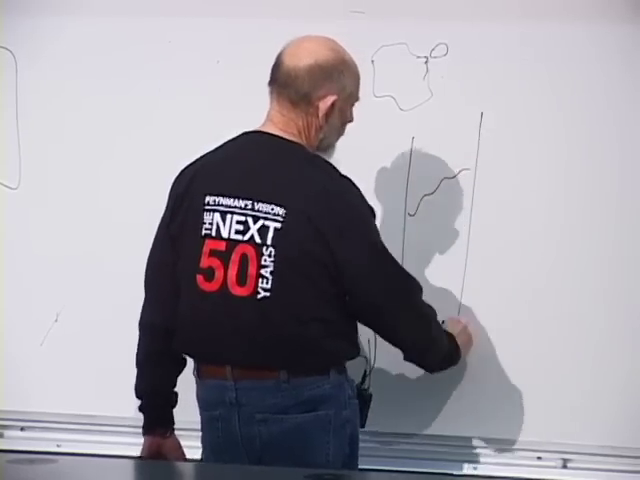
\includegraphics[width=0.72\textwidth]{lecture_06_figure_03.png}\caption{Los diagramas de intercambio completados en la pizarra: hay un acoplamiento en la emisión y otro en la absorción.}\lectureframe{00:11:30.000}\end{figure}

La versión de teoría de cuerdas sustituye el fotón por un gravitón y la carga eléctrica por \(g_s\). Un factor acompaña a la emisión y otro a la absorción, de modo que la intensidad de la interacción gravitatoria escala como \(g_s^2\).

A grandes distancias, la misma interacción debe reproducir la ley de fuerza de Newton,
\begin{equation}
F_{\mathrm{grav}}\sim G_N\frac{M_1M_2}{r^2}.
\end{equation}
Las masas y la dependencia inversa del cuadrado describen las fuentes y la propagación; aquí nos interesa el acoplamiento que las multiplica.

\begin{figure}[htbp]\centering
\begin{tikzpicture}[x=1cm,y=1cm]
  \node[font=\small\bfseries] at (1.8,3.55) {electromagnetism};
  \draw[line width=0.8pt] (0,0) -- (0,3);
  \draw[line width=0.8pt] (3.6,0) -- (3.6,3);
  \draw[line width=0.8pt] plot[smooth] coordinates {(0,1.5) (0.45,1.72) (0.9,1.28) (1.35,1.72) (1.8,1.28) (2.25,1.72) (2.7,1.28) (3.15,1.72) (3.6,1.5)};
  \node[below] at (0,1.42) {\(e\)};
  \node[below] at (3.6,1.42) {\(e\)};
  \node[font=\small] at (1.8,0.25) {exchange strength \(\propto e^2\)};
  \node[font=\small\bfseries] at (7.2,3.55) {string gravity};
  \draw[line width=0.8pt,rounded corners=6pt] (5.4,0) -- (5.2,0.7) -- (5.5,1.5) -- (5.25,2.3) -- (5.4,3);
  \draw[line width=0.8pt,rounded corners=6pt] (9,0) -- (9.2,0.7) -- (8.9,1.5) -- (9.15,2.3) -- (9,3);
  \draw[line width=0.8pt] plot[smooth] coordinates {(5.5,1.5) (5.95,1.72) (6.4,1.28) (6.85,1.72) (7.3,1.28) (7.75,1.72) (8.2,1.28) (8.65,1.72) (8.9,1.5)};
  \node[below] at (5.5,1.42) {\(g_s\)};
  \node[below] at (8.9,1.42) {\(g_s\)};
  \node[font=\small] at (7.2,0.25) {exchange strength \(\propto g_s^2\)};
\end{tikzpicture}\caption{La analogía del recuento de acoplamientos. Cada extremo del cuanto intercambiado aporta un factor de interacción.}\end{figure}

Esta observación casi determina la constante de Newton. El acoplamiento \(g_s\) es adimensional, mientras que, en cuatro dimensiones, \(G_N\) tiene dimensiones de longitud al cuadrado. La única longitud microscópica disponible es \(\ell_s\); por tanto,
\begin{equation}
G_N\sim g_s^2\ell_s^2.
\label{eq:l06-newton-string}
\end{equation}
Al combinar esto con la ecuación~\eqref{eq:l06-planck-area}, se obtiene
\begin{equation}
\ell_p\sim g_s\ell_s.
\label{eq:l06-planck-string}
\end{equation}

\begin{figure}[htbp]\centering
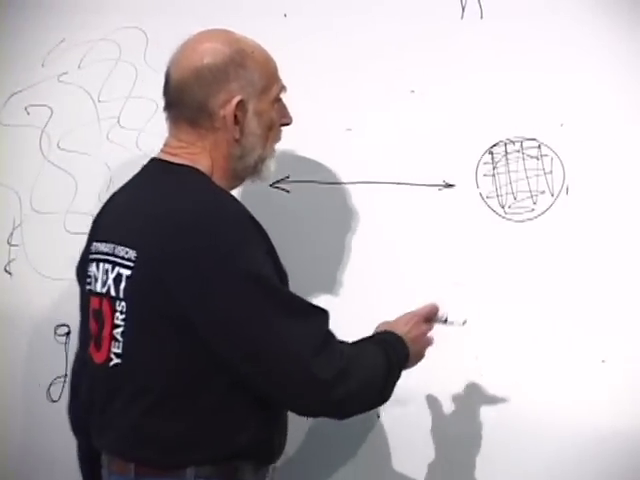
\includegraphics[width=0.72\textwidth]{lecture_06_figure_04.png}\caption{Las relaciones básicas que se conservan en la pizarra: \(\ell_p^2=G_N\) y \(\ell_p\sim g_s\ell_s\).}\lectureframe{00:15:45.000}\end{figure}

La ecuación~\eqref{eq:l06-newton-string} es la relación simplificada que usaremos a lo largo de esta clase.\editorialnote{En una teoría de cuerdas compactificada, la constante de Newton efectiva en cuatro dimensiones también depende del volumen de compactificación y de convenciones de orden unidad. La clase omite esos datos para aislar la dependencia de escala de la correspondencia.}

\begin{classroomqa}\audiencequestion{¿Es \(g_s\) mayor o menor que uno, y cuál de las longitudes es mayor?\lecturetimestamp{00:16:00}}\lecturerresponse{Trabajaremos a acoplamiento débil, \(g_s<1\). Entonces, \(\ell_p\sim g_s\ell_s\) implica que la longitud de cuerda es mayor que la longitud de Planck. El acoplamiento fuerte requiere otra descripción, que aquí no necesitamos.}\end{classroomqa}

\section{El recuento de los agujeros negros}

Si omitimos la constante de Boltzmann y los factores numéricos, la entropía de Bekenstein--Hawking es
\begin{equation}
S_{\mathrm{BH}}=\frac{A}{4G_N}sim\frac{A}{G_N}sim\frac{A}{\ell_p^2}.
\label{eq:l06-bh-area}
\end{equation}
El factor \(1/4\) es exacto en la fórmula semiclásica, pero no desempeñará ningún papel en este argumento de escala.

\begin{classroomqa}\audiencequestion{¿El subíndice ``BH'' significa agujero negro o Bekenstein--Hawking?\lecturetimestamp{00:16:51}}\lecturerresponse{Para nuestros propósitos puede recordarnos ambas cosas. Lo importante es que la entropía es el área del horizonte medida en unidades del área de Planck.}\end{classroomqa}

Para un agujero negro de Schwarzschild en cuatro dimensiones,
\begin{equation}
R_s=2G_NM,
\qquad
A=4\pi R_s^2.
\end{equation}
Omitiendo \(2\) y \(4\pi\), como hace la clase,
\begin{align}
S_{\mathrm{BH}}
&\sim \frac{R_s^2}{G_N}
\sim \frac{(G_NM)^2}{G_N} \\
&\sim M^2G_N
\sim M^2\ell_p^2.
\label{eq:l06-bh-mass}
\end{align}
Esta es la expresión que compararemos con el recuento de cuerdas.

\section{Una cuerda larga como paseo aleatorio}

Empecemos con una cuerda pequeña y aportémosle energía. Una cuerda genérica muy excitada no permanece como un bucle ordenado. Se convierte en un objeto largo y enredado, como un sedal tras enredarse mal en el carrete. El enredo tiene entropía porque hay una enorme cantidad de configuraciones que, macroscópicamente, parecen iguales.

Para contarlas, reemplacemos el espacio por una retícula cuyos enlaces tienen longitud \(\ell_s\). Los sitios son los vértices, los enlaces son las líneas y las celdas elementales son las plaquetas. Una cuerda se representa mediante una sucesión conexa de enlaces. Este modelo es deliberadamente rudimentario, pero su recuento exponencial de estados capta la dependencia de escala que buscamos.

\begin{figure}[htbp]\centering
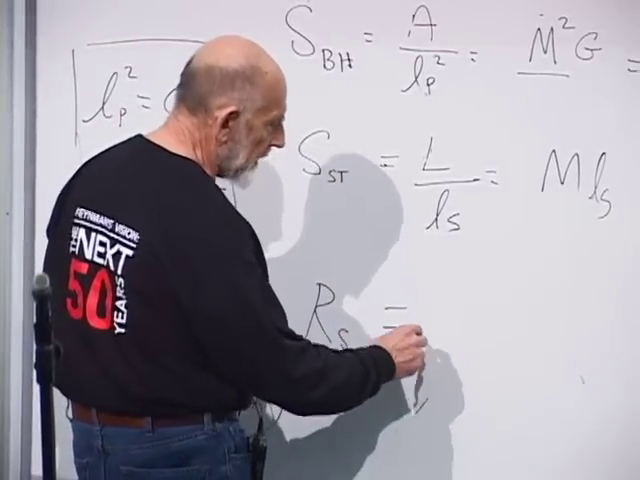
\includegraphics[width=0.72\textwidth]{lecture_06_figure_05.png}\caption{El modelo de retícula bidimensional. El segmento azul marca un paso de la cuerda; en cada sitio se cuentan las cuatro continuaciones posibles.}\lectureframe{00:23:50.000}\end{figure}

\begin{classroomqa}\audiencequestion{¿Cuántas opciones hay en cada paso del paseo simplificado?\lecturetimestamp{00:22:43}}\lecturerresponse{Cuatro en la retícula cuadrada, porque se permite retroceder inmediatamente. En tres dimensiones habría seis. Si se usa otra retícula cambia el número concreto, pero no el hecho de que la cantidad de paseos crece exponencialmente con el número de enlaces.}\end{classroomqa}

Si la cuerda tiene \(n\) enlaces, el recuento del modelo bidimensional es
\begin{equation}
\Omega_n\sim4^n.
\label{eq:l06-walk-count}
\end{equation}
Hay un paseo rectilíneo excepcional, pero es un solo estado entre \(4^n\). Un paseo típico se pliega una y otra vez y ocupa una bola enredada. Para valores grandes de \(n\), casi todas las configuraciones generadas al azar tienen un aspecto cualitativamente similar.

La entropía es el logaritmo del número de configuraciones indistinguibles macroscópicamente:
\begin{equation}
S_{\mathrm{st}}=\log\Omega_n\sim n\log4\sim n.
\label{eq:l06-string-entropy-n}
\end{equation}

\begin{classroomqa}\audiencequestion{¿Por qué la entropía resulta proporcional a \(n\) y no a \(4^n\)?\lecturetimestamp{00:25:39}}\lecturerresponse{La entropía es el logaritmo del número de estados. Así, \(\log(4^n)=n\log4\), y el factor \(\log4\) es una constante de orden unidad que omitiremos.}\end{classroomqa}

Si \(L\) es la longitud de contorno, obtenida siguiendo la cuerda de un extremo al otro, entonces
\begin{equation}
n=\frac{L}{\ell_s},
\qquad
S_{\mathrm{st}}\sim\frac{L}{\ell_s}.
\label{eq:l06-string-entropy-length}
\end{equation}
Aquí, \(L\) no es el diámetro de la bola enredada. Es la distancia mucho mayor medida a lo largo de la cuerda.

A continuación, sustituimos la longitud de contorno por la masa. Con \(c=\hbar=1\), la masa tiene dimensiones de inverso de longitud. Por tanto, un enlace del tamaño de una cuerda tiene una masa del orden de
\begin{equation}
m_{\mathrm{link}}\sim\frac{1}{\ell_s}.
\label{eq:l06-link-mass}
\end{equation}

\begin{classroomqa}\audiencequestion{¿Por qué la masa de un enlace debe escalar como \(1/\ell_s\)?\lecturetimestamp{00:29:20}}\lecturerresponse{En estas unidades, la masa es el inverso de una longitud, y \(\ell_s\) es la única longitud disponible. De forma equivalente, una tensión de cuerda del orden de \(1/\ell_s^2\) multiplicada por una longitud de enlace \(\ell_s\) da el mismo resultado.}\end{classroomqa}

La cuerda completa tiene entonces
\begin{equation}
M\sim n m_{\mathrm{link}}
\sim\frac{n}{\ell_s}
\sim\frac{L}{\ell_s^2},
\qquad
L\sim M\ell_s^2.
\label{eq:l06-string-mass}
\end{equation}
Al sustituir en la ecuación~\eqref{eq:l06-string-entropy-length} se obtiene
\begin{equation}
S_{\mathrm{st}}\sim M\ell_s.
\label{eq:l06-string-entropy-mass}
\end{equation}
El paseo por la retícula ignora las restricciones de la hoja de mundo y los coeficientes numéricos, pero el crecimiento exponencial del espectro de cuerdas muy excitadas da la misma escala dominante.\editorialnote{La construcción mediante un paseo aleatorio sirve como recurso mnemotécnico para la densidad de estados de cuerda a niveles altos; no es una discretización literal de una cuerda fundamental.}

\section{La discrepancia que pone en marcha el argumento}

Ahora tenemos las dos respuestas:
\begin{equation}
S_{\mathrm{BH}}\sim M^2\ell_p^2,
\qquad
S_{\mathrm{st}}\sim M\ell_s.
\label{eq:l06-two-entropies}
\end{equation}
Se parecen, pero no son iguales para una masa fija y un acoplamiento arbitrario. La expresión del agujero negro es cuadrática en \(M\); la de la cuerda es lineal. No podemos declarar sin más que una cuerda caliente es un agujero negro sin explicar cómo se conectan ambos regímenes.

\begin{figure}[htbp]\centering
\includegraphics[width=0.78\textwidth]{lecture_06_figure_06.png}\caption{La comparación despejada en la pizarra: arriba, la entropía del agujero negro; abajo, la entropía de la cuerda larga, y a la izquierda se conservan las relaciones entre Planck--cuerda.}\lectureframe{00:33:20.000}\end{figure}

Aquí se detuvo la clase. El suspenso es útil: la discrepancia no refuta la idea, sino que indica que hay que comparar el mismo estado mientras se modifica la intensidad de la gravedad.

\section{Girar el mando del acoplamiento}

Mantengamos fijo \(\ell_s\) e imaginemos que podemos variar \(g_s\). Para \(g_s=0\), las cuerdas no se dividen ni se unen, y la gravedad desaparece porque \(G_N\sim g_s^2\ell_s^2\). En ese caso, un estado suficientemente energético es una cuerda larga que interactúa débilmente.

Aumentemos \(g_s\) lentamente. Las interacciones de cuerdas se vuelven posibles y, lo que es más importante para el argumento actual, la gravedad se intensifica.

\begin{classroomqa}\audiencequestion{Al aumentar \(g_s\), ¿el primer efecto es simplemente que la cuerda se divide en cuerdas más cortas?\lecturetimestamp{00:36:29}}\lecturerresponse{La escisión y la unión se vuelven posibles, pero mantengamos fijo \(\ell_s\) y sigamos el estado de alta entropía. El efecto central es que aumenta \(G_N\), de modo que la autogravedad de la cuerda larga atrae hacia dentro la bola enredada.}\end{classroomqa}

El objeto se contrae y se vuelve más denso. Su energía potencial gravitatoria es negativa, así que la contracción reduce su energía total y, por tanto, su masa.

\begin{classroomqa}\audiencequestion{¿La energía aumenta o disminuye cuando la autogravedad atrae la cuerda?\lecturetimestamp{00:37:48}}\lecturerresponse{Disminuye. La energía de enlace se vuelve más negativa. La masa a lo largo del recorrido no tiene por qué mantenerse constante, aunque sigamos el mismo estado.}\end{classroomqa}

Con el tiempo, el tamaño del objeto se vuelve comparable a su radio de Schwarzschild. A partir de ese punto, la descripción mediante un agujero negro es la más natural. Una excitación inicial mayor alcanza esta condición con un acoplamiento menor, porque un objeto más masivo necesita menos intensidad gravitatoria para formar un horizonte.

\begin{figure}[htbp]\centering
\resizebox{0.95\linewidth}{!}{%
\begin{tikzpicture}[x=1cm,y=1cm,>=Latex]
  \draw[->,line width=0.9pt] (0,0) -- (11,0) node[right] {increasing \(g_s\)};
  \node[draw,rounded corners,align=center,minimum width=2.6cm,minimum height=1.15cm] at (1.8,1.5) {long excited string\\weak self-gravity};
  \node[draw,rounded corners,align=center,minimum width=2.6cm,minimum height=1.15cm] at (5.5,1.5) {correspondence point\\\(R_s\sim\ell_s\)};
  \node[draw,circle,align=center,minimum size=1.8cm] at (9.3,1.5) {black\\hole};
  \draw[->,line width=0.8pt] (3.15,1.5) -- (4.1,1.5) node[midway,above,font=\small] {contracts};
  \draw[->,line width=0.8pt] (6.9,1.5) -- (8.25,1.5);
  \node[font=\small,align=center] at (5.5,-0.65) {same family of states followed slowly;\\binding energy and mass may change};
\end{tikzpicture}}\caption{La trayectoria de correspondencia a \(\ell_s\) fijo. Invertir la flecha transforma el estado de agujero negro en un estado de cuerda larga.}\end{figure}

\begin{classroomqa}\audiencequestion{¿Debemos imaginar que \(g_s\) varía entre cero y uno?\lecturetimestamp{00:40:18}}\lecturerresponse{Sí. El argumento permanece en el régimen de acoplamiento débil. Si \(g_s\) es muy pequeño, el estado debe tener una masa correspondientemente grande antes de convertirse en un agujero negro. No hace falta entrar en el régimen \(g_s>1\), cuyo control teórico es deficiente.}\end{classroomqa}

En este experimento mental, el cambio lento es reversible.

\begin{classroomqa}\audiencequestion{Si reducimos de nuevo el acoplamiento hasta que la gravedad ya no pueda mantener unido el agujero negro, ¿en qué se convierte?\lecturetimestamp{00:41:37}}\lecturerresponse{En una cuerda larga. Cuando la gravedad se anula, todo lo que aparece en esta construcción debe describirse mediante estados de cuerda. Al girar el mando en un sentido, se transforma una cuerda en un agujero negro; al girarlo en el sentido contrario, un agujero negro se transforma en una cuerda.}\end{classroomqa}

A energía total y volumen fijos, la configuración dominante de alta entropía es, esencialmente, una sola cuerda larga en vez de una cantidad enorme de cuerdas cortas. Esto no se demuestra aquí. Es un resultado de la mecánica estadística de las cuerdas cerca del régimen de Hagedorn y volveremos a estudiarlo.

\section{Lo que observa alguien desde el exterior}

¿Dónde está la cuerda cuando el objeto se describe como un agujero negro? En la descripción exterior no desaparece de golpe. El tiempo de Schwarzschild lleva el cruce aparente a tiempos arbitrariamente tardíos, así que los grados de libertad de cuerda se representan como acumulados sobre el horizonte o cerca de él.

\begin{figure}[htbp]\centering
\includegraphics[width=0.72\textwidth]{lecture_06_figure_07.png}\caption{Comparación en la pizarra entre un horizonte macroscópico, donde la estructura a escala de cuerda es una capa tenue, y un horizonte más pequeño cuyo radio se aproxima a la escala del bucle.}\lectureframe{00:45:30.000}\end{figure}

Para \(R_s\gg\ell_s\), el agujero negro es macroscópico y la estructura a escala de cuerda forma apenas una capa delgada en relación con el radio del horizonte. Cuando el radio disminuye y se acerca a \(\ell_s\), pierde sentido distinguir entre un agujero negro suave y una cuerda extendida. Esta es una descripción exterior, basada en un horizonte estirado; no debe confundirse con la afirmación, independiente de las coordenadas, de que la materia en caída nunca cruza un horizonte regular.\editorialnote{La clase emplea la descripción exterior habitual en la complementariedad de los agujeros negros. La expresión ``sobre el horizonte'' designa grados de libertad resueltos en la descripción exterior, no una derivación independiente de su ubicación covariante.}

La transición ocurre cuando
\begin{equation}
R_s\sim\ell_s.
\label{eq:l06-correspondence-radius}
\end{equation}
Por debajo de la escala de cuerda, la geometría de Schwarzschild no puede resolver la estructura que supuestamente la sustenta. Los bucles fluctúan y se alejan del horizonte que habría de formarse, y resulta más apropiado llamar cuerda al estado.

\section{El punto de correspondencia}

Usamos \(R_s\sim G_NM\) en la ecuación~\eqref{eq:l06-correspondence-radius}:
\begin{equation}
G_NM\sim\ell_s.
\end{equation}
A continuación, sustituimos \(G_N\sim g_s^2\ell_s^2\):
\begin{equation}
M g_s^2\ell_s^2\sim\ell_s,
\qquad
M g_s^2\ell_s\sim1.
\label{eq:l06-correspondence-condition}
\end{equation}

\begin{figure}[htbp]\centering
\includegraphics[width=0.72\textwidth]{lecture_06_figure_08.png}\caption{El álgebra completa de la transición en la pizarra: \(R_s\sim\ell_s\) conduce a la condición adimensional recuadrada \(Mg_s^2\ell_s\sim1\).}\lectureframe{00:49:50.000}\end{figure}

Alguien del público advirtió lo que anticipa esta condición. En el punto de correspondencia,
\begin{align}
S_{\mathrm{BH}}
&\sim M^2\ell_p^2
\sim M^2g_s^2\ell_s^2 \\
&=(M\ell_s)(Mg_s^2\ell_s)
\sim M\ell_s
\sim S_{\mathrm{st}}.
\label{eq:l06-entropy-preview}
\end{align}

\begin{classroomqa}\audiencequestion{¿Las ecuaciones ya implican que las entropías del agujero negro y de la cuerda se vuelven iguales?\lecturetimestamp{00:50:18}}\lecturerresponse{Sí. Justamente hacia eso conduce el cálculo. Ya hemos reunido los elementos en la pizarra, pero la clase aplaza su ensamblaje completo para repasar con cuidado la lógica de la correspondencia.}\end{classroomqa}

La ecuación~\eqref{eq:l06-entropy-preview} es el anticipo algebraico, en una línea, implícito en el intercambio. Establece la dependencia de escala, no el coeficiente exacto \(1/4\). Para obtener igualdades microscópicas exactas hacen falta agujeros negros cuyo análisis esté mejor controlado y construcciones de cuerdas más detalladas.\editorialnote{La clase termina antes de presentar la ecuación~\eqref{eq:l06-entropy-preview} como una derivación completa. La escribimos aquí porque alguien del público señala explícitamente la igualdad y ya han aparecido todas las relaciones necesarias.}

\section{Por qué se conserva la entropía en el proceso}

Queda un ingrediente lógico. Supongamos que variamos suficientemente despacio un parámetro de control, como un campo magnético o \(g_s\), mientras el sistema está aislado y la evolución es reversible. La energía, el tamaño y la energía de enlace pueden cambiar, pero la entropía se conserva:
\begin{equation}
\Delta S=0.
\label{eq:l06-adiabatic-entropy}
\end{equation}
La clase relaciona esto con la conservación de la información. La entropía mide la información que queda oculta en una descripción macroscópica; un cambio lento y reversible del hamiltoniano reorganiza los estados sin eliminar esa información.

\begin{classroomqa}\audiencequestion{¿Para que la entropía sea constante, el recorrido debe evitar una transición de fase?\lecturetimestamp{00:54:01}}\lecturerresponse{Sí, debe ser posible seguir el estado de manera continua. Un sistema finito no presenta una transición de fase termodinámica estrictamente no analítica del tipo que ocurre en el límite de volumen infinito; si el cambio es suficientemente lento, la correspondencia puede tratarse como una transición gradual y suave.}\end{classroomqa}

Aquí se usa «adiabático» en el sentido más estricto de un proceso cuasiestático y reversible. Un proceso adiabático irreversible puede generar entropía; la lentitud y la posibilidad de seguir el estado son esenciales.\editorialnote{La afirmación termodinámica \(\Delta S=0\) exige un proceso adiabático reversible. En mecánica cuántica, la idea correspondiente consiste en seguir el mismo conjunto de estados a medida que cambia un parámetro, sin transiciones entre niveles que no estén controladas.}

\begin{classroomqa}\audiencequestion{¿Por qué una sola cuerda larga debería tener más entropía que varias cuerdas más cortas con la misma masa total?\lecturetimestamp{00:54:44}}\lecturerresponse{Es contraintuitivo, pero el recuento explícito de estados a altas energías favorece una componente de cuerda larga en un volumen fijo. La demostración se aplaza; para el argumento actual solo necesitamos que el agujero negro se transforme en el sector de cuerdas de máxima entropía, y no en un gas diluido de muchísimas cuerdas cortas.}\end{classroomqa}

Por tanto, la estrategia operativa es:
\begin{enumerate}\item Empezar con un agujero negro de masa \(M_0\) y acoplamiento \(g_{s,0}\).
\item Reducir \(g_s\) lentamente mientras se sigue la misma familia de estados de alta entropía.
\item Detenerse en \(R_s\sim\ell_s\), donde la descripción del agujero negro se convierte en una descripción mediante una cuerda larga.
\item Contar los estados de cuerda usando \(S_{\mathrm{st}}\sim M\ell_s\).
\item Transportar esa entropía de vuelta al agujero negro original a lo largo del proceso reversible.
\end{enumerate}

\begin{figure}[htbp]\centering
\includegraphics[width=0.72\textwidth]{lecture_06_figure_09.png}\caption{El principio que se conserva en la pizarra al enunciar la estrategia: un cambio adiabático de \(g_s\) no modifica \(S\).}\lectureframe{00:56:40.000}\end{figure}

La teoría de cuerdas ha producido recuentos de entropía mucho más precisos para agujeros negros cargados, en rotación, supersimétricos, casi extremales y de dimensiones superiores. La discusión del agujero negro neutro de Schwarzschild que presentamos aquí es el argumento aproximado de correspondencia: identifica la densidad paramétrica de estados y la transición física, pero no una degeneración exacta protegida.\editorialnote{La concordancia exacta es más sólida para ciertos agujeros negros especiales cuyos recuentos de estados están protegidos cuando cambia el acoplamiento. Esta clase presenta deliberadamente la versión más sencilla, a orden de magnitud.}

\begin{classroomqa}\audiencequestion{Al anular la gravedad, ¿podría el estado convertirse en dos cuerdas en vez de exactamente en una?\lecturetimestamp{00:58:25}}\lecturerresponse{Hay una probabilidad finita de que se formen unas pocas cuerdas largas, y usar dos en lugar de una no cambia la escala dominante de la entropía. Lo que sí cambiaría el argumento sería la fragmentación en un enorme gas de cuerdas cortas; el recuento estadístico a altas energías no favorece ese resultado.}\end{classroomqa}

El agujero negro es la configuración de máxima entropía que puede concentrarse en una región, y la cuerda larga es el estado correspondiente de alta entropía cuando se elimina la gravedad. Ya hemos conectado ambas descripciones, pero aún no hemos desarrollado un cálculo de precisión. El siguiente paso es repetir el álgebra con cuidado y preguntarnos hasta qué punto es fiable la correspondencia.

\chapter{Entropía de los agujeros negros, holografía y espacio de de Sitter}

\lectureoverview{Completamos el argumento de correspondencia iniciado en la clase anterior. La entropía de una cuerda muy excitada es proporcional a su masa, mientras que la de un agujero negro de Schwarzschild es proporcional a su área. Las dos fórmulas no se relacionan identificando un agujero negro con gravedad intensa con una cuerda libre, sino variando lentamente el acoplamiento de cuerda hasta que ambas descripciones coincidan. La ley del área conduce entonces de forma natural al principio holográfico. En la parte final de la clase se introduce el espacio en expansión y la geometría de de Sitter, cuyo horizonte estudiaremos en la siguiente clase.}

\section{Volvamos al problema de contar}

Quedaba un cabo suelto en el recuento de cuerdas largas. Si se reparte una longitud total fija entre varias cuerdas, las cuerdas idénticas de la misma longitud son indistinguibles. Sin embargo, sus posiciones en la caja forman parte del estado, y se elige una caja cuyo tamaño sea aproximadamente el de la región que ocupa la correspondiente cuerda larga individual.

\begin{classroomqa}
\audiencequestion{¿Las cuerdas cortas se distinguen unas de otras? ¿Se cuentan sus posiciones?\lecturetimestamp{00:00:37}}
\lecturerresponse{Las cuerdas con propiedades idénticas son indistinguibles, pero sus posiciones en la caja sí se cuentan. La comparación se hace a volumen fijo, elegido para que coincida con la región que ocupa la cuerda larga.}
\end{classroomqa}

Una vez aclarado esto, podemos enunciar el objetivo. Reuniremos una breve lista de ecuaciones y las usaremos para obtener la dependencia de la entropía de los agujeros negros. No hacen falta integrales ni sumas infinitas. La dificultad no es algebraica: consiste en saber qué magnitudes se pueden comparar y en qué etapa del argumento.

\section{Unidades naturales y área de Planck}

Fijemos
\begin{equation}
c=\hbar=1,
\label{eq:l07-natural-units}
\end{equation}
pero mantengamos explícita la constante de Newton. La primera consecuencia es que el tiempo y la longitud tienen las mismas unidades. La relación del fotón
\begin{equation}
E=\frac{\hbar c}{\lambda}
\end{equation}
y la relación entre masa y energía \(E=mc^2\) implican entonces
\begin{equation}
[M]=L^{-1}.
\label{eq:l07-mass-dimension}
\end{equation}
Por tanto, la masa puede expresarse como el inverso de una longitud.

\begin{figure}[htbp]
\centering
\includegraphics[width=0.62\textwidth]{lecture_07_figure_02.png}
\caption{Convención de unidades naturales al comienzo del argumento dimensional. La fórmula de la energía se completa en las ecuaciones anteriores.}
\lectureframe{00:03:27.900}
\end{figure}

Para determinar las unidades de \(G_N\), usemos la aceleración newtoniana solo como recurso para llevar la cuenta dimensional:
\begin{equation}
a\sim\frac{G_NM}{R^2}.
\end{equation}
Como \(T\) y \(L\) tienen las mismas unidades, \([a]=L/T^2=L^{-1}\). Junto con la ecuación~\eqref{eq:l07-mass-dimension}, esto da
\begin{equation}
[G_N]=L^2.
\end{equation}
En estas unidades, la constante de Newton tiene dimensiones de área. Si definimos la longitud de Planck como
\begin{equation}
G_N=\ell_p^2,
\label{eq:l07-planck-area}
\end{equation}
se entiende enseguida por qué \(A/G_N=A/\ell_p^2\) es adimensional: mide un área en unidades de áreas de Planck.

\section{El acoplamiento de cuerda y la intensidad de la gravedad}

Ahora debemos expresar la gravedad en términos de cuerdas. La imagen útil es la de un proceso de intercambio. Cuando una cuerda se cruza consigo misma, puede dividirse y volver a unirse. Un objeto puede emitir un pequeño bucle de cuerda cerrada y otro absorberlo; si esa excitación es un gravitón, el proceso media la interacción gravitatoria. En la emisión aparece un factor de interacción y en la absorción aparece otro, así que la intensidad del intercambio incluye \(g_s^2\).

El acoplamiento \(g_s\) es adimensional. Más precisamente, es un acoplamiento a nivel de amplitud, mientras que una probabilidad o una tasa empiezan en el orden \(g_s^2\).\editorialnote{En la clase, a veces se llama probabilidad a \(g_s\) y luego se corrige esa afirmación: se trata de la raíz cuadrada de una probabilidad. El acoplamiento perturbativo corresponde al nivel de amplitud.} Como \(G_N\) tiene dimensiones de área, aún falta una escala de longitud. La longitud fundamental de cuerda \(\ell_s\), que fija la escala de una ondulación elemental de la cuerda, la proporciona:
\begin{equation}
G_N\sim g_s^2\ell_s^2,
\qquad
\ell_p\sim g_s\ell_s.
\label{eq:l07-planck-string}
\end{equation}

\begin{figure}[htbp]
\centering
\includegraphics[width=0.72\textwidth]{lecture_07_figure_05.png}
\caption{La relación entre acoplamientos escrita en la pizarra: \(G_N=\ell_p^2\) y \(g_s^2\ell_s^2\sim\ell_p^2\).}
\lectureframe{00:12:15.000}
\end{figure}

A acoplamiento débil, \(g_s\ll1\), la longitud de Planck es mucho menor que la longitud de cuerda. Reducir \(g_s\) debilita la gravedad y deja fija la escala de la cuerda elemental.\editorialnote{En una teoría efectiva de cuatro dimensiones, los datos de compactificación y las convenciones numéricas también intervienen en \(G_N\). En este argumento de escala se mantienen fijos y se omiten.}

\section{El recuento de una cuerda larga}

La entropía cuenta las decisiones elementales necesarias para especificar un estado. Reemplacemos una cuerda muy excitada por un paseo en una retícula cuadrada. En cada vértice, el siguiente enlace puede apuntar en una de cuatro direcciones. Describir la elección elemental como una decisión entre cuatro opciones o como dos decisiones binarias solo cambia una constante de orden unidad. Lo que importa es el número de pasos.

Si \(L\) es la longitud de contorno de la cuerda y cada paso tiene longitud \(\ell_s\), entonces hacen falta
\begin{equation}
N=\frac{L}{\ell_s}
\end{equation}
pasos. El número de paseos crece exponencialmente, de forma esquemática como \(\Omega_N\sim q^N\), con \(q\) de orden unidad; por tanto,
\begin{equation}
S_{\mathrm{str}}=\log\Omega_N\sim N\sim\frac{L}{\ell_s}.
\label{eq:l07-string-entropy-length}
\end{equation}

\begin{figure}[htbp]
\centering
\includegraphics[width=0.68\textwidth]{lecture_07_figure_03.png}

\vspace{0.7em}
\begin{tikzpicture}[scale=0.82]
  \draw[step=0.8cm,gray!45,thin] (0,0) grid (6.4,4.0);
  \draw[very thick,blue!60!black]
    (0.8,0.8)--(1.6,0.8)--(1.6,1.6)--(2.4,1.6)--(2.4,2.4)--
    (3.2,2.4)--(3.2,1.6)--(4.0,1.6)--(4.0,2.4)--(4.8,2.4)--
    (4.8,3.2)--(5.6,3.2);
  \draw[<->,thick] (0.8,-0.35)--(1.6,-0.35);
  \node[below] at (1.2,-0.35) {step \(\ell_s\)};
  \node[align=center] at (8.1,2.0) {\(N=L/\ell_s\) steps\\[0.3em]\(S_{\mathrm{str}}\sim N\)};
\end{tikzpicture}
\caption{El modelo reticular de la pizarra y su interpretación depurada como paseo aleatorio. El número de elecciones lo determina la longitud de contorno, no el diámetro de la bola enmarañada.}
\lectureframe{00:17:20.000}
\end{figure}

La masa se cuenta a partir de los mismos segmentos elementales. Un segmento de longitud \(\ell_s\) tiene una escala de masa
\begin{equation}
m_{\mathrm{seg}}\sim\frac{1}{\ell_s}.
\end{equation}

\begin{classroomqa}
\audiencequestion{¿Se asigna al segmento elemental la longitud \(\ell_s\)?\lecturetimestamp{00:18:56}}
\lecturerresponse{Sí. Su longitud característica es \(\ell_s\), de modo que, en unidades naturales, su masa característica es \(1/\ell_s\).}
\end{classroomqa}

Al sumar las masas de los segmentos \(L/\ell_s\) se obtiene
\begin{equation}
M\sim\frac{L}{\ell_s}\frac{1}{\ell_s}
=\frac{L}{\ell_s^2},
\qquad
L\sim M\ell_s^2.
\label{eq:l07-string-mass}
\end{equation}
Esta relación de escala condensa las energías cinética y potencial de la cuerda oscilante; un tratamiento detallado de mecánica estadística da la misma dependencia. Al sustituir en la ecuación~\eqref{eq:l07-string-entropy-length} obtenemos la fórmula de la cuerda que necesitaremos:
\begin{equation}
S_{\mathrm{str}}\sim M\ell_s.
\label{eq:l07-string-entropy-mass}
\end{equation}

\begin{figure}[htbp]
\centering
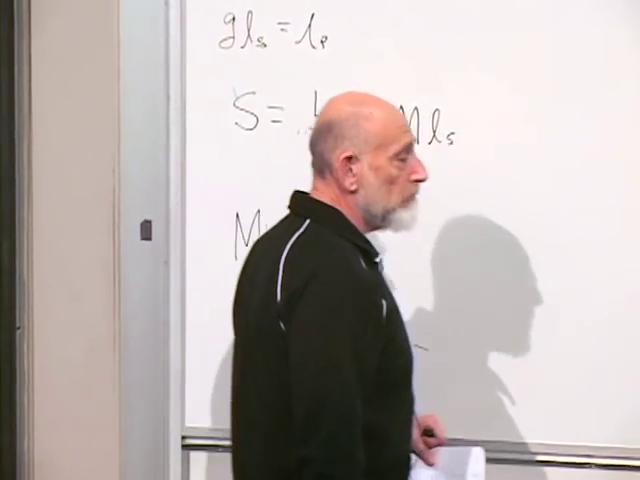
\includegraphics[width=0.66\textwidth]{lecture_07_figure_04.png}
\caption{La columna correspondiente a la cuerda, reunida antes de la comparación: \(\ell_p\sim g_s\ell_s\), \(S_{\mathrm{str}}\sim L/\ell_s\sim M\ell_s\) y \(M\sim L/\ell_s^2\).}
\lectureframe{00:21:57.800}
\end{figure}

\section{Por qué una cuerda libre todavía no es un agujero negro}

En el lado gravitatorio, la fórmula semiclásica exacta es
\begin{equation}
S_{\mathrm{BH}}=\frac{A}{4G_N}.
\label{eq:l07-bh-exact}
\end{equation}

\begin{classroomqa}
\audiencequestion{¿Qué coeficiente numérico va en el denominador?\lecturetimestamp{00:23:28}}
\lecturerresponse{Cuatro. El argumento de correspondencia recuperará la dependencia de escala, pero es demasiado aproximado para determinar ese factor exacto.}
\end{classroomqa}

Para un agujero negro de Schwarzschild en cuatro dimensiones,
\begin{equation}
R_s=2G_NM,
\qquad
A=4\pi R_s^2.
\end{equation}
Si omitimos las constantes numéricas, como hace la clase,
\begin{align}
S_{\mathrm{BH}}
&\sim\frac{A}{G_N}
\sim\frac{(G_NM)^2}{G_N} \\
&\sim M^2G_N
\sim M^2\ell_p^2.
\label{eq:l07-bh-scaling}
\end{align}

\begin{figure}[htbp]
\centering
\includegraphics[width=0.72\textwidth]{lecture_07_figure_06.png}
\caption{La comparación completa en la pizarra: la entropía de la cuerda tiene dimensiones de longitud en unidades de cuerda, mientras que la del agujero negro tiene dimensiones de área en unidades de Planck.}
\lectureframe{00:25:35.000}
\end{figure}

El parecido entre las ecuaciones~\eqref{eq:l07-string-entropy-mass} y \eqref{eq:l07-bh-scaling} resulta sugerente, pero no son la misma fórmula. No sería correcto llamar cuerda libre al agujero negro original y sustituir sin más. El recuento de la cuerda libre omite la interacción atractiva entre sus partes, precisamente la interacción que la compacta hasta formar un agujero negro y reduce su energía total mediante una energía de enlace negativa.

Un ejemplo estelar permite reconocer el error. Un gas caliente con la masa de una estrella, colocado en una caja demasiado grande, no es un modelo de estrella, ni siquiera si tiene la misma temperatura. La autogravedad modifica el tamaño de equilibrio y la relación entre energía y entropía. Seguir todas las auto-interacciones de una cuerda larga sería difícil, así que evitaremos hacerlo.

\begin{classroomqa}
\audiencequestion{Si un bucle pequeño sale de una cuerda larga, su entropía disminuye. ¿Significa eso que el intercambio de gravitones reduce la entropía del sistema gravitatorio?\lecturetimestamp{00:28:48}}
\lecturerresponse{No en el proceso de intercambio en equilibrio que consideramos aquí. Las excitaciones virtuales se emiten y se absorben en ambas direcciones; el esquema no representa la pérdida literal de un fragmento permanente de cuerda. Por ahora, su único propósito es establecer los dos factores de acoplamiento y, por tanto, la dependencia en \(g_s^2\).}
\end{classroomqa}

\section{El ejercicio de correspondencia adiabática}

Empecemos, en cambio, en un régimen donde la gravedad es despreciable. Cuando \(g_s\to0\), las cuerdas se cruzan sin dividirse ni unirse y desaparece la atracción gravitatoria propia. Aumentemos \(g_s\) manteniendo fijo \(\ell_s\): la gravedad se fortalece, una cuerda muy excitada se contrae y, con el tiempo, se convierte en un agujero negro. Si giramos lentamente el dial en sentido contrario, el agujero negro debe volver a un estado de cuerda. Podría convertirse en unas pocas cuerdas largas, pero el recuento de altas energías de la clase anterior indica que el sector dominante contiene una cuerda larga, no un gas enorme de cuerdas cortas.

\begin{classroomqa}
\audiencequestion{¿Qué se mantiene fijo mientras cambia el acoplamiento?\lecturetimestamp{00:32:19}}
\lecturerresponse{La longitud de cuerda \(\ell_s\) y, por tanto, la escala de masa de la cuerda elemental \(1/\ell_s\). El dial modifica \(g_s\) y, por consiguiente, \(G_N\sim g_s^2\ell_s^2\).}
\end{classroomqa}

El cambio debe ser lento, aislado y reversible. En esas condiciones, la entropía es un invariante adiabático:
\begin{equation}
\Delta S=0.
\label{eq:l07-adiabatic}
\end{equation}
La lentitud por sí sola no basta si tienen lugar transiciones disipativas o incontroladas. Aquí, ``adiabático'' significa que se puede seguir continuamente la misma familia de estados.\editorialnote{Este es el sentido termodinámico de adiabático, en el que el proceso es reversible. Un proceso irreversible puede ser adiabático en el sentido de que no hay flujo de calor y, aun así, producir entropía.}

Sea el agujero negro objetivo de masa \(M_0\) y acoplamiento \(g_{s,0}\). Antes de usar la fórmula del área que intentamos explicar, el análisis dimensional solo permite afirmar que la entropía de un agujero negro neutro y sin rotación es alguna función de la combinación adimensional
\begin{equation}
S_{\mathrm{BH}}=f(M\ell_p)
=f(Mg_s\ell_s).
\label{eq:l07-entropy-function}
\end{equation}
A \(\ell_s\) fijo, una trayectoria isentrópica mantiene
\begin{equation}
Mg_s=M_0g_{s,0}
\label{eq:l07-adiabat}
\end{equation}
constante, siempre que se siga la misma rama de estados.

Al disminuir \(g_s\), se elimina energía de enlace negativa, así que la masa \(M\) aumenta a lo largo de esta trayectoria. La configuración de cuerda subyacente también queda menos ligada y se expande. Sin embargo, a lo largo de la adiabat, el radio de Schwarzschild formal se comporta como \(R_s\sim Mg_s^2\ell_s^2\sim g_s\ell_s\) y, por tanto, disminuye.\editorialnote{En la explicación oral se usa ``crece'' para referirse al objeto liberado de su enlace gravitatorio. No debe interpretarse como una afirmación de que el radio de Schwarzschild crezca a lo largo de la adiabat derivada.}

\begin{classroomqa}
\audiencequestion{¿El objeto crece o se encoge al debilitarse la gravedad?\lecturetimestamp{00:36:28}}
\lecturerresponse{La estructura de cuerda se libera y se expande, mientras que la masa aumenta porque se elimina energía de enlace negativa. El radio asignado por la fórmula del agujero negro disminuye hasta alcanzar la escala de cuerda, donde esa descripción del agujero negro deja de ser útil.}
\end{classroomqa}

\section{Dos curvas y su intersección}

Representemos la masa en el eje vertical y el acoplamiento de cuerda en el horizontal. La ecuación~\eqref{eq:l07-adiabat} es una hipérbola: \(M\propto g_s^{-1}\).

\begin{classroomqa}
\audiencequestion{¿Qué tipo de curva tiene producto constante \(Mg_s\)?\lecturetimestamp{00:44:08}}
\lecturerresponse{Una hipérbola. Es la adiabat que pasa por el punto objetivo \((g_{s,0},M_0)\).}
\end{classroomqa}

La segunda curva marca la transición entre descripciones. Un agujero negro no puede describirse mediante una geometría convencional de Schwarzschild cuando su radio es menor que el de una ondulación elemental de cuerda. Por eso estimamos el punto de correspondencia mediante
\begin{equation}
R_s\sim\ell_s.
\label{eq:l07-correspondence-radius}
\end{equation}
Al usar \(R_s\sim MG_N\) y la ecuación~\eqref{eq:l07-planck-string}, esto queda
\begin{equation}
Mg_s^2\ell_s^2\sim\ell_s,
\qquad
Mg_s^2\sim\frac{1}{\ell_s}.
\label{eq:l07-transition-curve}
\end{equation}
Así, la curva de transición decrece como \(M\propto g_s^{-2}\), más deprisa que la adiabat.

\begin{figure}[htbp]
\centering
\includegraphics[width=0.70\textwidth]{lecture_07_figure_07.png}

\vspace{0.6em}
\begin{tikzpicture}[x=1cm,y=0.78cm]
  \draw[->] (0.4,0.4)--(7.0,0.4) node[right] {\(g_s\)};
  \draw[->] (0.4,0.4)--(0.4,6.5) node[above] {\(M\)};
  \draw[thick,black] plot[smooth] coordinates {(1.0,5.6) (1.5,4.0) (2.2,2.9) (3.2,2.1) (4.6,1.55) (6.3,1.2)};
  \draw[very thick,red!70!black] plot[smooth] coordinates {(1.25,6.0) (1.55,4.55) (2.0,3.15) (2.7,2.0) (3.8,1.25) (5.8,0.78)};
  \fill (2.05,3.1) circle (2pt) node[above right] {\((g_{s,*},M_*)\)};
  \node[black,rotate=-17] at (4.75,1.9) {\(Mg_s=M_0g_{s,0}\)};
  \node[red!70!black,rotate=-25] at (4.45,0.95) {\(Mg_s^2=1/\ell_s\)};
  \node at (5.75,3.5) {black hole};
  \node at (1.15,1.25) {string};
\end{tikzpicture}
\caption{El gráfico de la pizarra y su interpretación depurada. La adiabat negra corta la curva de correspondencia roja, más pronunciada, en el punto donde el objeto adquiere carácter de cuerda.}
\lectureframe{00:49:35.000}
\end{figure}

En la intersección \((M_*,g_{s,*})\), las dos ecuaciones son
\begin{align}
M_*g_{s,*} &= M_0g_{s,0}, \\
M_*g_{s,*}^2 &\sim \frac{1}{\ell_s}.
\end{align}
Elevemos al cuadrado la primera ecuación y dividamos por la segunda:
\begin{equation}
M_*
\sim M_0^2g_{s,0}^2\ell_s.
\end{equation}
Al multiplicar por \(\ell_s\),
\begin{equation}
M_*\ell_s
\sim M_0^2g_{s,0}^2\ell_s^2
\sim M_0^2G_{N,0}.
\label{eq:l07-crossover-result}
\end{equation}

\begin{figure}[htbp]
\centering
\includegraphics[width=0.68\textwidth]{lecture_07_figure_08.png}
\caption{El álgebra completa de la transición, incluido \(M_*\ell_s=M_0^2g_{s,0}^2\ell_s^2=M_0^2G_{N,0}\).}
\lectureframe{00:54:40.000}
\end{figure}

\begin{classroomqa}
\audiencequestion{Al dividir las ecuaciones de las dos curvas, ¿\(\ell_s\) queda en el numerador o en el denominador?\lecturetimestamp{00:52:41}}
\lecturerresponse{En el numerador. Dividir por \(1/\ell_s\) equivale a multiplicar por \(\ell_s\), y por eso \(M_*\sim M_0^2g_{s,0}^2\ell_s\).}
\end{classroomqa}

En la transición es válida la fórmula de la cuerda, así que
\begin{equation}
S_*\sim M_*\ell_s.
\end{equation}
La entropía no cambió a lo largo de la trayectoria. Al combinar esta afirmación con la ecuación~\eqref{eq:l07-crossover-result} obtenemos la entropía del agujero negro objetivo original:
\begin{equation}
S_{\mathrm{BH}}(M_0)
\sim M_0^2G_{N,0}
\sim M_0^2\ell_{p,0}^2.
\label{eq:l07-final-correspondence}
\end{equation}
Esta es la dependencia deseada según la ley del área.

\section{Qué demuestra y qué no demuestra la correspondencia}

Esta construcción no afirma que el agujero negro original, con su intensa gravedad, sea una cuerda libre. Lleva el objeto a un régimen donde el recuento de cuerdas es fiable, obtiene allí la entropía y la transporta de vuelta a lo largo de una trayectoria reversible. La transición es un cruce gradual, no una frontera de fase claramente definida, así que esta estimación no permite determinar el coeficiente \(1/4\) de la ecuación~\eqref{eq:l07-bh-exact}.

El mismo razonamiento funciona, no obstante, de forma paramétrica para los agujeros negros cargados, los objetos negros en otras dimensiones y las branas negras extendidas. En ejemplos con más simetría y supersimetría se pueden contar estados protegidos que conservan información exacta al variar el acoplamiento; esos métodos recuperan los coeficientes numéricos, pero requieren herramientas matemáticas que no hacen falta para el argumento conceptual de hoy.

Lo más importante es que el cálculo proporciona una interpretación microscópica. La entropía es una señal de que existe una estructura oculta. La mecánica de fluidos describe densidad, presión y flujo sin mostrar las moléculas; la entropía del fluido revela la existencia de esos grados de libertad microscópicos. De manera similar, la relatividad general describe un horizonte sin mostrar sus microestados. El recuento de cuerdas muestra que una teoría cuántica coherente de la gravedad puede contener suficientes estados para dar cuenta de la entropía de los agujeros negros.

\begin{classroomqa}
\audiencequestion{¿Qué habría significado \(S\sim M^3\ell_p^3\), en lugar del resultado cuadrático?\lecturetimestamp{00:59:41}}
\lecturerresponse{Habría tenido la forma de una ley de volumen. La entropía de la materia ordinaria en una habitación o en una taza de café es proporcional al volumen; la respuesta cuadrática es especial porque, mediante \(R_s\sim M\ell_p^2\), es proporcional al área del horizonte.}
\end{classroomqa}

El resultado indica que la entropía de Bekenstein--Hawking no es una mera analogía termodinámica formal. Apunta a grados de libertad gravitatorios microscópicos, aunque la derivación elemental no los haga visibles uno por uno.

\section{De la entropía máxima a la holografía}

Ahora cambiamos de pregunta. En vez de preguntar por la entropía de un estado dado, preguntamos cuál es la entropía máxima compatible con una región.

Empecemos con un modelo reticular corriente de una habitación. Dividamos el volumen en celdas de tamaño \(V_{\mathrm{cell}}\) y asignemos a cada celda una pregunta de sí o no: ¿está ocupada o vacía? Susskind da al átomo imaginario el nombre deliberadamente absurdo de ``meatonium'', para que ningún detalle atómico realista distraiga del recuento. Si
\begin{equation}
N=\frac{V}{V_{\mathrm{cell}}},
\end{equation}
entonces el número de configuraciones y la entropía máxima son
\begin{equation}
\Omega=2^N,
\qquad
S_{\max}=\log\Omega=N\log2
\sim\frac{V}{V_{\mathrm{cell}}}.
\label{eq:l07-volume-count}
\end{equation}

\begin{figure}[htbp]
\centering
\includegraphics[width=0.68\textwidth]{lecture_07_figure_09.png}
\caption{La habitación, dividida en celdas, con dos estados por celda. Esto cuenta la entropía máxima, no la entropía de la habitación ordenada que ocupa la clase.}
\lectureframe{01:05:20.000}
\end{figure}

La habitación real está muy por debajo de este máximo. Un estado que recorriera caóticamente todas esas opciones de las celdas estaría extremadamente caliente. Lo que se conserva del modelo simplificado es la expectativa habitual de que el número de grados de libertad independientes y, por tanto, la entropía máxima escalan con el volumen.

La gravedad trastoca esa expectativa. Consideremos una región esférica de área de frontera \(A\), entropía inicial \(S_{\mathrm{i}}\) y masa \(M\), menor que la masa \(M_{\mathrm{BH}}\) de un agujero negro que llenaría justo la esfera. Si \(M\) fuera mayor, su horizonte ya se extendería más allá de la frontera elegida.

Enviemos ahora una capa esférica de masa \(M_{\mathrm{BH}}-M\). Su composición es irrelevante: la clase contempla que sea de luz, de materia ordinaria o incluso de queso suizo. Dispongamos que colapse. El estado final es un agujero negro cuyo horizonte llena justo la región y cuya entropía es
\begin{equation}
S_{\mathrm{f}}=\frac{A}{4G_N}.
\end{equation}
La segunda ley exige que
\begin{equation}
S_{\mathrm{i}}\le S_{\mathrm{f}}
=\frac{A}{4G_N}.
\label{eq:l07-holographic-bound}
\end{equation}

\begin{figure}[htbp]
\centering
\includegraphics[width=0.70\textwidth]{lecture_07_figure_10.png}

\vspace{0.5em}
\begin{tikzpicture}[scale=0.88]
  \draw[thick] (0,0) circle (1.35);
  \draw[very thick,red!70!black] (0,0) circle (2.05);
  \fill[gray!25] (0,0) circle (1.32);
  \node at (0,0) {\(M,S_{\mathrm{i}}\)};
  \draw[-{Latex[length=3mm]},thick,red!70!black] (3.5,0)--(2.15,0);
  \node[align=center,right] at (3.5,0) {incoming shell\\\(M_{\mathrm{BH}}-M\)};
  \node[below] at (0,-2.2) {final horizon area \(A\)};
\end{tikzpicture}
\caption{La construcción con la capa esférica. Se envía hacia dentro masa adicional suficiente para formar un agujero negro cuyo horizonte llena justo la región seleccionada.}
\lectureframe{01:13:30.000}
\end{figure}

Como un agujero negro de ese tamaño es un estado permitido y satura la desigualdad, la entropía máxima es
\begin{equation}
S_{\max}=\frac{A}{4G_N}.
\label{eq:l07-holographic-maximum}
\end{equation}
Esta es la formulación en términos de recuento del principio holográfico: el número máximo de grados de libertad independientes en una región gravitatoria escala con el área de su frontera; en orden de magnitud, corresponde a un grado de libertad por área de Planck, y no al número de volúmenes de Planck interiores.\editorialnote{El argumento de la capa esférica supone que la región puede encerrarse y colapsar de la manera indicada. Los espaciotiempos más generales requieren cotas covariantes de entropía, pero el argumento esférico recoge el principio empleado en la clase.}

La diferencia es enorme. La intuición de la teoría de campos local sugiere que las elecciones hechas en distintos puntos interiores deberían combinarse de forma independiente y producir una ley de volumen. La gravedad dice que un número suficiente de esas elecciones se colapsaría por sí solo, y el agujero negro ofrece la entropía admisible máxima. Por tanto, el recuento de frontera no es una pequeña corrección al recuento de volumen: supone una organización distinta del espacio de Hilbert.

\begin{classroomqa}
\audiencequestion{¿Qué ocurre en un universo muy grande con una densidad aproximadamente uniforme?\lecturetimestamp{01:15:48}}
\lecturerresponse{Esa pregunta requiere cosmología, no la construcción esférica estática. Motiva el paso inmediato a las soluciones en expansión de las ecuaciones de Einstein.}
\end{classroomqa}

\begin{classroomqa}
\audiencequestion{¿Está relacionada la cota del área con el principio de incertidumbre?\lecturetimestamp{01:16:03}}
\lecturerresponse{La clase deja esta pregunta abierta y pasa a la cosmología.}
\end{classroomqa}

\section{El espacio en expansión}

Aquí no deduciremos las soluciones cosmológicas a partir de las ecuaciones de Einstein; las escribiremos y aprenderemos a interpretarlas. Las secciones espaciales pueden tener curvatura positiva y ser cerradas, curvatura negativa y ser hiperbólicas, o ser planas. Para esta explicación consideremos secciones espaciales euclidianas planas en un espaciotiempo dependiente del tiempo.

\begin{classroomqa}
\audiencequestion{¿Cuál es el análogo espaciotemporal del espacio euclidiano ordinario?\lecturetimestamp{01:19:37}}
\lecturerresponse{El espacio de Minkowski. La cosmología que consideramos aquí tiene secciones espaciales planas, pero no es un espaciotiempo de Minkowski, porque su métrica espacial cambia con el tiempo.}
\end{classroomqa}

La conocida imagen del globo describe una superficie cerrada en expansión y de una dimensión menos. Susskind recuerda que intentó hacer la demostración con un globo grande marcado; el rotulador debilitó la goma y provocó un estallido literal. El percance también pone al descubierto un defecto conceptual de la analogía. Cuando un globo ordinario se expande, sus moléculas de goma se separan y el material se adelgaza hasta romperse. En el espacio cosmológico, las leyes locales no se diluyen. Para que la analogía funcione, hay que imaginar que se insertan continuamente moléculas de goma nuevas, de modo que cada pequeña zona conserve las mismas propiedades locales. En un modelo plano, sustituyamos el globo por una gran lámina que se estira uniformemente y se repone de manera análoga.

Matemáticamente, la expansión se incorpora a la métrica:
\begin{equation}
\begin{aligned}
ds^2&=-dt^2+a(t)^2d\mathbf{x}^2,\\
d\mathbf{x}^2&=\delta_{ij}\,dx^i dx^j
=dx^2+dy^2+dz^2.
\end{aligned}
\label{eq:l07-frw-metric}
\end{equation}

\begin{figure}[htbp]
\centering
\includegraphics[width=0.72\textwidth]{lecture_07_figure_11.png}
\caption{La métrica de expansión espacial plana tal como está escrita en la pizarra.}
\lectureframe{01:25:10.000}
\end{figure}

Los puntos cuyas coordenadas espaciales permanecen fijas se llaman comóviles. Si dos puntos comóviles tienen una separación coordenada \(\Delta x\), su distancia propia en el instante \(t\) es
\begin{equation}
D(t)=a(t)\Delta x.
\label{eq:l07-proper-distance}
\end{equation}
Sus coordenadas no cambian, pero sí cambia la distancia métrica entre ellos. Al derivar manteniendo fijo \(\Delta x\),
\begin{equation}
V=\dot D=\dot a\,\Delta x
=\frac{\dot a}{a}D.
\end{equation}
Definamos el parámetro de Hubble
\begin{equation}
H(t)=\frac{\dot a(t)}{a(t)}.
\label{eq:l07-hubble-parameter}
\end{equation}
Entonces,
\begin{equation}
V=H(t)D,
\label{eq:l07-hubble-law}
\end{equation}
que es la ley de Hubble en un instante cósmico fijo.

\begin{figure}[htbp]
\centering
\includegraphics[width=0.68\textwidth]{lecture_07_figure_12.png}
\caption{La ley de recesión a tiempo igual escrita en la pizarra: \(V=D\,\dot a/a\).}
\lectureframe{01:29:10.000}
\end{figure}

La expresión ``constante de Hubble'' puede llevar a confusión. En general, \(H(t)\) cambia con el tiempo. Lo que es constante espacialmente es la razón \(V/D\) para cada par de puntos comóviles en una misma sección temporal.

\begin{classroomqa}
\audiencequestion{En el caso de las galaxias lejanas, ¿a qué instante corresponde el tiempo de esta relación? Las observamos en una época anterior.\lecturetimestamp{01:31:10}}
\lecturerresponse{La ecuación~\eqref{eq:l07-hubble-law} es una afirmación válida a tiempo igual. Una observación sigue un rayo de luz dirigido hacia el pasado y, por ello, detecta la galaxia lejana en un instante anterior. Así que la relación entre el corrimiento al rojo medido y la distancia requiere conocer toda la historia del cono de luz, no un único valor instantáneo de \(H\).}
\end{classroomqa}

\begin{figure}[htbp]
\centering
\includegraphics[width=0.66\textwidth]{lecture_07_figure_13.png}
\caption{El esquema espaciotemporal empleado para distinguir una separación a tiempo igual de lo que observa alguien a lo largo de un rayo de luz dirigido hacia el pasado.}
\lectureframe{01:33:20.000}
\end{figure}

\section{La escala de Hubble y la expansión de de Sitter}

En unidades \(c=1\), la ecuación~\eqref{eq:l07-hubble-law} asigna una velocidad de recesión igual a la velocidad de la luz a la distancia
\begin{equation}
D_H=\frac{1}{H}.
\label{eq:l07-hubble-radius}
\end{equation}
Puntos comóviles más lejanos pueden tener \(V>1\), e incluso \(V\gg1\), sin violar la relatividad especial. No pasan junto a un observador local a una velocidad mayor que la de la luz: su separación propia aumenta porque se expande la geometría intermedia.\editorialnote{En una cosmología general dependiente del tiempo, \(1/H\) es el radio de Hubble, pero no es automáticamente un horizonte de sucesos. En el caso de de Sitter que veremos a continuación, sí es la escala constante del horizonte.}

En muchos modelos cosmológicos antiguos con expansión desacelerada, \(H(t)\) disminuye y \(1/H(t)\) aumenta, de modo que regiones que antes se alejaban a velocidad superlumínica pueden entrar más tarde en contacto causal. En cambio, la imagen de tiempos tardíos que se analiza en la clase se aproxima a un valor positivo constante \(H\). Entonces \(1/H\) permanece fijo y la ecuación de expansión pasa a ser
\begin{equation}
\frac{\dot a}{a}=H,
\qquad
\dot a=Ha.
\label{eq:l07-constant-h}
\end{equation}

\begin{classroomqa}
\audiencequestion{¿Qué unidades tiene un parámetro de Hubble constante?\lecturetimestamp{01:38:24}}
\lecturerresponse{El inverso del tiempo. De manera equivalente, cuando \(c=1\), es el inverso de una longitud. La magnitud \(H^{-1}\) proporciona tanto una escala temporal de expansión como una escala de distancia; la clase usa como ejemplo un valor aproximado de quince mil millones de años.}
\end{classroomqa}

La solución de la ecuación~\eqref{eq:l07-constant-h} es
\begin{equation}
a(t)=a_0e^{Ht}.
\label{eq:l07-desitter-scale-factor}
\end{equation}

\begin{classroomqa}
\audiencequestion{¿Qué función tiene una tasa de variación proporcional a sí misma?\lecturetimestamp{01:39:04}}
\lecturerresponse{Una exponencial. Por tanto, el factor de escala es \(a_0e^{Ht}\), mientras que el coeficiente espacial \(a(t)^2\) de la métrica crece como \(e^{2Ht}\).}
\end{classroomqa}

\begin{figure}[htbp]
\centering
\includegraphics[width=0.70\textwidth]{lecture_07_figure_14.png}
\caption{Las ecuaciones con \(H\) constante y su solución exponencial, escritas en la pizarra.}
\lectureframe{01:39:30.000}
\end{figure}

Un espaciotiempo con esta expansión exponencial es el espacio de de Sitter. Su escala de Hubble constante produce un horizonte de sucesos a una distancia propia finita. En cierto sentido, esta geometría complementa la imagen del agujero negro: un observador permanece dentro de un horizonte cosmológico, mientras los objetos suficientemente lejanos se alejan y nunca pueden enviar señales que alcancen al observador. El horizonte de un agujero negro oculta el interior a un observador exterior; el horizonte de de Sitter oculta el exterior de la región accesible al observador. A diferencia de un agujero negro ordinario que se evapora, aquí se considera que la geometría ideal de de Sitter persiste. Aquí apenas comienza la comparación. La siguiente clase desarrolla el horizonte, su termodinámica y los enigmas que plantea para la cosmología.

\chapter{Energía del vacío y horizontes de de Sitter}

\lectureoverview{La energía del vacío no se comporta como la materia ordinaria: no selecciona un sistema de referencia inercial privilegiado ni se diluye a medida que se expande el universo. Al incluir la gravedad, ese cero de energía aparentemente inocuo modifica la geometría del espacio-tiempo. Deduciremos la ley dominada por la materia \(a(t)\propto t^{2/3}\), la contrastaremos con la ley dominada por el vacío \(a(t)\propto e^{Ht}\) y, a continuación, reescribiremos el espacio-tiempo de de Sitter en coordenadas conformes. El diagrama causal resultante revela un horizonte de sucesos dependiente del observador, situado a una distancia propia fija.}

\section{Fluctuaciones cuánticas del vacío}

Empezamos con la pregunta que motiva toda la lección. La teoría cuántica de campos asigna energía al espacio vacío. ¿Significa esto que pares reales de electrón--positrón surgen continuamente de la nada?

\begin{classroomqa}
\audiencequestion{¿Se producen y aniquilan realmente pares de electrón--positrón en el vacío, o es solo un recurso contable?\lecturetimestamp{00:00:06}}
\lecturerresponse{Los pares virtuales contribuyen a la energía del vacío, pero no son partículas ordinarias que podamos observar surgir del espacio vacío. Son fluctuaciones del estado fundamental cuántico y persisten solo dentro de los límites propios de un proceso virtual.}
\end{classroomqa}

El oscilador armónico ofrece el modelo más sencillo. Clásicamente, puede permanecer inmóvil en el mínimo de su potencial. En mecánica cuántica, la posición exactamente en el mínimo y el momento exactamente nulo son incompatibles. El estado fundamental representa un compromiso entre ambos y conserva la energía de punto cero
\begin{equation}
E_0=\frac{1}{2}\hbar\omega.
\label{eq:l08-zero-point}
\end{equation}
Esta es la energía mínima que puede tener el oscilador. No es un estado excitado ni representa un flujo de partículas observables.

Un campo libre se descompone en modos normales, cada uno de los cuales se comporta como un oscilador. El campo electromagnético en una cavidad es un ejemplo conocido. Cada modo aporta un término de la forma de la ecuación~\eqref{eq:l08-zero-point}; los campos cuánticos del electrón, los quarks y otras partículas aportan sus propias fluctuaciones del estado fundamental. La suma de estas contribuciones da lugar a lo que llamamos energía del vacío. La célebre discrepancia entre las estimaciones microscópicas ingenuas y la escala cosmológica observada es real, pero no es el tema de esta lección.

\begin{classroomqa}
\audiencequestion{¿Se volverá a tratar la discrepancia de aproximadamente \(120\) órdenes de magnitud?\lecturetimestamp{00:02:59}}
\lecturerresponse{Aquí no. El objetivo de esta lección es entender los horizontes cósmicos: cómo las ecuaciones cosmológicas producen expansión acelerada y por qué esta crea horizontes de sucesos.}
\end{classroomqa}

\begin{classroomqa}
\audiencequestion{¿Forma parte de la discusión de esta noche la relación ultravioleta--infrarroja de la lección anterior?\lecturetimestamp{00:03:59}}
\lecturerresponse{Quizá volvamos a tratarla más adelante, pero no forma parte del argumento previsto. El recorrido inmediato va de la energía del vacío a la cosmología y, después, a los horizontes.}
\end{classroomqa}

\section{Por qué la energía del vacío es invariante de Lorentz}

La siguiente pregunta parece elemental, pero pone de manifiesto la propiedad que define la energía del vacío. Si el espacio vacío tiene una densidad de energía positiva, ¿por qué no se comporta como un medio óptico y modifica la velocidad de la luz?

\begin{classroomqa}
\audiencequestion{¿Debería una densidad positiva de energía del vacío tener un efecto refractivo y hacer que la luz viajara un poco más despacio?\lecturetimestamp{00:04:35}}
\lecturerresponse{La materia ordinaria puede producir ese efecto porque define un sistema de reposo privilegiado. La energía del vacío es distinta: no selecciona tal sistema, y todos los observadores inerciales obtienen la misma densidad de energía del vacío. Por eso, las mediciones locales de la luz siguen dando la velocidad invariante \(c\).}
\end{classroomqa}

Debemos distinguir entre una simetría de las leyes y una simetría de un estado particular. Las ecuaciones de la física pueden ser invariantes bajo traslaciones aunque Stanford no sea Berkeley y la Tierra no sea el espacio interestelar. Trasladar \emph{toda} la configuración física deja intactas las leyes; la distribución real de la materia no tiene por qué ser igual en todos los lugares. Del mismo modo, que las ecuaciones sean invariantes bajo rotaciones no hace que esta aula tenga simetría rotacional.

La misma distinción se aplica a las transformaciones de Lorentz. Un gas tiene un sistema de reposo. Un observador que se mueve a través de él ve moléculas en movimiento y una densidad de energía distinta, de modo que el estado del gas no es invariante de Lorentz, aunque sí lo sean las ecuaciones que lo rigen. La materia ordinaria, los baños de radiación y los aparatos de laboratorio rompen la simetría al seleccionar movimientos o direcciones especiales.

La energía del vacío es la forma excepcional de materia que no lo hace. Imaginemos un detector que mide la densidad de energía del vacío. En reposo, obtiene cierto valor \(\rho_{\rm vac}\). Aceleremos el detector y repitamos la medición: el resultado no cambia. En notación relativista, esta propiedad se expresa mediante un tensor de tensiones proporcional a la métrica,
\begin{equation}
T_{\mu\nu}^{\rm vac}=-\rho_{\rm vac}g_{\mu\nu},
\qquad
p_{\rm vac}=-\rho_{\rm vac}.
\label{eq:l08-vacuum-stress}
\end{equation}
\editorialnote{La relación entre presión y densidad no se deduce en la pizarra. Es la formulación covariante de las dos propiedades que definen el tema de la lección: la invariancia de Lorentz y la densidad constante durante la expansión.}

La precisión sobre el carácter local es importante. Un rayo de luz que pasa junto a un observador se mide con relojes y reglas cercanos y se encuentra que viaja a \(c\). Preguntar por la velocidad de un rayo lejano con respecto a nosotros en una geometría en expansión requiere elegir coordenadas y un procedimiento para comparar sucesos distantes. Esa velocidad coordenada no tiene por qué ser igual a \(c\), aunque todo observador local mida \(c\).

\begin{classroomqa}
\audiencequestion{En esta discusión, ¿son sinónimos la energía del vacío y la constante cosmológica?\lecturetimestamp{00:11:57}}
\lecturerresponse{Sí. Son dos formas de colocar el mismo término en las ecuaciones de Einstein: puede describirse como una constante cosmológica en el lado geométrico o como energía-momento del vacío invariante de Lorentz en el lado de las fuentes.}
\end{classroomqa}

\section{Qué se diluye y qué no}

Llenemos una región grande con partículas no relativistas de masa \(m\). En escalas suficientemente grandes como para promediar sobre galaxias y cúmulos, supongamos que la distribución es homogénea. Si un volumen comóvil contiene \(N\) partículas, su densidad de materia es
\begin{equation}
\rho_m=\frac{Nm}{V}.
\end{equation}
Cuando se duplican todas las dimensiones lineales, el volumen aumenta por un factor de \(2^3=8\), mientras que \(N\) y \(m\) permanecen constantes. Por tanto, la densidad se reduce a un octavo de su valor inicial. La materia ordinaria se diluye porque las mismas partículas ocupan un volumen físico mayor.

La radiación también se diluye, y más rápidamente. Su densidad numérica disminuye con el volumen, mientras que la longitud de onda de cada fotón se estira y su energía experimenta un corrimiento al rojo. Más adelante anotaremos el resultado \(\rho_r\propto a^{-4}\), pero esta noche no resolveremos la cosmología dominada por la radiación.

La energía del vacío es la excepción:
\begin{equation}
\rho_{\rm vac}(t)=\text{constant}.
\label{eq:l08-rho-vac-constant}
\end{equation}
No se agrupa, no selecciona una dirección ni un sistema de referencia inercial, y su densidad no disminuye cuando el espacio se expande. Si una caja comóvil aumenta de tamaño, la energía del vacío que contiene aumenta en proporción a su volumen.

\editorialnote{Que la densidad sea constante no significa que la energía total del vacío dentro de una caja comóvil en expansión también lo sea. La conservación covariante de la energía-momento,
\(\dot\rho+3H(\rho+p)=0\), se cumple porque la energía del vacío tiene presión negativa \(p_{\rm vac}=-\rho_{\rm vac}\). El término de trabajo proporciona exactamente la variación de la energía total del vacío en la caja.}

\section{La gravedad percibe el cero de energía}

En la física de laboratorio sin gravedad, sumar la misma constante a todas las energías por lo general no cambia nada. Los espectros dependen de diferencias: la energía entre un átomo excitado y uno no excitado, o entre un estado con una partícula y otro sin ella. El espacio vacío parece no ofrecer ninguna referencia con la cual medir su energía absoluta.

La gravedad cambia la cuestión. La masa es energía, la energía es fuente de gravedad y, por tanto, la energía del vacío gravita. Una constante invisible en una transición atómica puede curvar el espacio-tiempo.

La ecuación de Einstein separa la geometría de las fuentes:
\begin{equation}
G_{\mu\nu}=8\pi G_N T_{\mu\nu},
\label{eq:l08-einstein}
\end{equation}
en unidades en las que \(c=1\). El tensor de Einstein \(G_{\mu\nu}\) se construye a partir de la métrica \(g_{\mu\nu}(x)\) y sus derivadas. El tensor de energía-momento \(T_{\mu\nu}\) contiene la densidad de energía, la densidad de momento, la presión y las tensiones de la materia y de los campos no gravitatorios. La energía del vacío pertenece a este lado de las fuentes, igual que la materia ordinaria.\editorialnote{La introducción oral asocia brevemente \(8\pi/3\) con la ecuación tensorial. El factor \(1/3\) corresponde a la ecuación de Friedmann espacialmente plana que aparece a continuación, no a la ecuación~\eqref{eq:l08-einstein}.}

\begin{figure}[htbp]
\centering
\includegraphics[width=0.62\textwidth]{lecture_08_figure_02.png}
\caption{El lado geométrico de la ecuación de Einstein, construido a partir de la métrica del espacio-tiempo \(g_{\mu\nu}(x)\).}
\lectureframe{00:21:58.820}
\end{figure}

\section{La geometría reducida a un factor de escala}

Elegimos ahora la geometría homogénea en expansión más sencilla, con secciones espaciales planas:
\begin{equation}
ds^2=-dt^2+a(t)^2\,d\mathbf{x}^2,
\qquad
d\mathbf{x}^2=dx^2+dy^2+dz^2.
\label{eq:l08-frw-metric}
\end{equation}
Las marcas coordenadas \(\mathbf{x}\) están pintadas sobre una lámina de goma infinita. No tienen por qué moverse, pero sus separaciones físicas sí cambian. Dos puntos comóviles separados por \(\Delta\mathbf{x}\) tienen, a \(t\) fijo, una distancia propia
\begin{equation}
D(t)=a(t)\lvert\Delta\mathbf{x}\rvert.
\label{eq:l08-proper-distance}
\end{equation}
Así, toda la dependencia temporal de esta geometría, altamente simétrica, queda contenida en una sola función: el factor de escala \(a(t)\). Un valor constante de \(a\) da lugar al espacio-tiempo plano de Minkowski tras un reescalamiento espacial. Un valor variable de \(a\) puede mantener plana cada sección espacial y, a la vez, curvar el espacio-tiempo completo.

\begin{classroomqa}
\audiencequestion{Para las marcas coordenadas \(x=7\) y \(x=13\), ¿su separación en coordenadas es \(4\)?\lecturetimestamp{00:27:40}}
\lecturerresponse{No. Es \(13-7=6\), por lo que su separación física es \(6a(t)\). Conviene precisar que \(x\) indica la posición comóvil, mientras que al multiplicarla por \(a(t)\) se obtiene la distancia física.}
\end{classroomqa}

Para esta métrica y una densidad de energía uniforme en el espacio, una componente de la ecuación de Einstein se convierte en la ecuación de Friedmann espacialmente plana,
\begin{equation}
\left(\frac{\dot a}{a}\right)^2
=\frac{8\pi G_N}{3}\rho(t).
\label{eq:l08-friedmann}
\end{equation}
El cociente
\begin{equation}
H(t)\equiv\frac{\dot a(t)}{a(t)}
\label{eq:l08-hubble-definition}
\end{equation}
es el parámetro de Hubble. En esta etapa es una definición y puede variar con el tiempo.

\begin{figure}[htbp]
\centering
\includegraphics[width=0.90\textwidth]{lecture_08_figure_03.png}
\caption{La métrica plana en expansión y la ecuación de Friedmann, tras restituir en la pizarra el factor \(1/a^2\) que faltaba.}
\lectureframe{00:30:30.000}
\end{figure}

\paragraph{La imagen del balance de energía.}
En esta imagen del balance de energía, la ecuación~\eqref{eq:l08-friedmann} se escribe de manera esquemática como
\begin{equation}
-\frac{3}{8\pi G_N}H^2+\rho=0.
\label{eq:l08-energy-heuristic}
\end{equation}
La energía de la materia es positiva, mientras que el grado de libertad gravitatorio representado por el factor de escala en expansión tiene un término cinético negativo. En este problema reducido, es útil recordar que la energía gravitatoria negativa más la energía positiva de la materia suman cero.

\editorialnote{La ecuación~\eqref{eq:l08-energy-heuristic} es la restricción hamiltoniana en un modelo de minisuperspace altamente simétrico; no es un teorema independiente de las coordenadas según el cual todo universo arbitrario tenga una energía total globalmente conservada e igual a cero. La lección la utiliza como interpretación heurística de la restricción de Friedmann.}

\section{Expansión dominada por la materia}

Volvamos a una caja matemática comóvil de lado coordenado \(\Delta x=1\). Su lado físico es \(a(t)\), de modo que su volumen físico es \(a(t)^3\). Si contiene \(N\) partículas no relativistas de masa \(m\), entonces
\begin{equation}
\rho_m(t)=\frac{Nm}{a(t)^3}
=\frac{\rho_0}{a(t)^3}.
\label{eq:l08-matter-density}
\end{equation}
Las partículas no se expanden; sí lo hace la separación media entre ellas.

\begin{figure}[htbp]
\centering
\includegraphics[width=0.84\textwidth]{lecture_08_figure_04.png}
\caption{La métrica y la ecuación de Friedmann a medida que se desarrolla el argumento de la caja comóvil.}
\lectureframe{00:36:07.940}
\end{figure}

Al sustituir en la ecuación~\eqref{eq:l08-friedmann} se obtiene
\begin{equation}
\left(\frac{\dot a}{a}\right)^2
=\frac{8\pi G_N\rho_0}{3a^3}.
\end{equation}
Escribamos \(K=8\pi G_N\rho_0/3\) y elijamos la rama en expansión:
\begin{align}
\dot a^2&=\frac{K}{a},\\
\dot a&=\sqrt{K}\,a^{-1/2},\\
a^{1/2}\,da&=\sqrt{K}\,dt.
\label{eq:l08-matter-separated}
\end{align}

\begin{classroomqa}
\audiencequestion{¿Cómo se resuelve la ecuación una vez separadas las variables?\lecturetimestamp{00:38:15}}
\lecturerresponse{Integramos ambos lados. La integral de \(a^{1/2}\,da\) es \(\frac{2}{3}a^{3/2}\), no \(\frac{3}{2}a^{3/2}\); \(\frac{3}{2}\) es la nueva potencia y \(\frac{2}{3}\) es el coeficiente.}
\end{classroomqa}

Por consiguiente,
\begin{equation}
\frac{2}{3}a^{3/2}
=\sqrt{K}\,(t-t_B),
\end{equation}
donde \(t_B\) es una constante de integración que fija el origen temporal elegido. Salvo por la normalización y el desplazamiento temporal,
\begin{equation}
a(t)\propto (t-t_B)^{2/3}.
\label{eq:l08-matter-solution}
\end{equation}

\begin{figure}[htbp]
\centering
\includegraphics[width=0.86\textwidth]{lecture_08_figure_05.png}
\caption{La sustitución de la densidad de materia y la separación de variables que conducen a \(a^{1/2}da\propto dt\).}
\lectureframe{00:38:30.000}
\end{figure}

La curva \(t^{2/3}\) crece más despacio que una recta. Su pendiente disminuye, así que un universo dominado por la materia se desacelera. En el lenguaje newtoniano empleado en la lección, las partículas empezaron a separarse y su atracción gravitatoria mutua reduce continuamente la tasa de separación.

\begin{figure}[htbp]
\centering
\includegraphics[width=0.86\textwidth]{lecture_08_figure_06.png}
\caption{Comparación en la pizarra de la expansión lineal con la ley de materia cóncava hacia abajo \(a(t)\propto t^{2/3}\).}
\lectureframe{00:40:00.000}
\end{figure}

Como referencia, un baño de radiación tiene
\begin{equation}
\rho_r\propto a^{-4},
\end{equation}
en lugar de \(a^{-3}\): la dilución por el volumen aporta tres potencias y el corrimiento cosmológico al rojo aporta una más. También se puede resolver el factor de escala correspondiente, pero la lección deja deliberadamente de lado ese ejercicio.

\section{Expansión dominada por el vacío}

Consideremos ahora solo la energía del vacío en el lado derecho de la ecuación de Friedmann. Como \(\rho_{\rm vac}\) es constante,
\begin{equation}
\left(\frac{\dot a}{a}\right)^2
=\frac{8\pi G_N}{3}\rho_{\rm vac}
\equiv H^2.
\label{eq:l08-de-sitter-friedmann}
\end{equation}
Hay que distinguir dos usos de \(H\). La ecuación~\eqref{eq:l08-hubble-definition} define la cantidad \(\dot a/a\), que puede depender del tiempo. La ecuación~\eqref{eq:l08-de-sitter-friedmann} indica que, en un universo compuesto solo por energía del vacío, su valor es la constante
\begin{equation}
H=\sqrt{\frac{8\pi G_N\rho_{\rm vac}}{3}}.
\end{equation}
Al elegir la rama en expansión, se obtiene
\begin{equation}
\dot a=Ha,
\end{equation}
y, por tanto,
\begin{equation}
a(t)=C e^{Ht}.
\label{eq:l08-exponential-solution}
\end{equation}
La constante de integración \(C\) fija la normalización arbitraria de las coordenadas comóviles. Un crecimiento proporcional al valor actual de \(a\) es un crecimiento exponencial.

\begin{figure}[htbp]
\centering
\includegraphics[width=0.88\textwidth]{lecture_08_figure_07.png}
\caption{La ecuación de vacío dominante \((\dot a/a)^2=H^2\), su forma de primer orden \(\dot a=Ha\) y la solución exponencial.}
\lectureframe{00:47:45.000}
\end{figure}

La ley de Hubble para objetos comóviles es
\begin{equation}
v_{\rm rec}=HD.
\label{eq:l08-hubble-law}
\end{equation}
En este caso de de Sitter puro, la distancia propia a la que la velocidad de recesión iguala \(c\) es constante:
\begin{equation}
D_H=\frac{c}{H},
\label{eq:l08-hubble-radius}
\end{equation}
o bien \(D_H=H^{-1}\) en las unidades \(c=1\) empleadas en la pizarra. Esta escala fija reaparecerá geométricamente como el radio del horizonte de sucesos de de Sitter.\editorialnote{En una cosmología arbitraria dependiente del tiempo, el radio de Hubble no es automáticamente un horizonte de sucesos. La identificación es válida aquí porque \(H\) es constante en el espacio de de Sitter exacto.}

La lección propone un experimento mental con un detector de energía del vacío. Coloquemos dos cuerpos de prueba muy ligeros, lejos de otras fuentes y inicialmente en reposo respecto del flujo comóvil, y hagamos que su atracción mutua sea despreciable. Su separación obedece la expansión exponencial. El efecto es demasiado pequeño para detectarlo con un aparato terrestre, pero las distancias cósmicas y el tiempo de retrospección permiten observar la misma física.

\section{De la dominación de la materia a la del vacío}

El modelo cosmológico real considerado en la lección contiene ambos términos:
\begin{equation}
H(t)^2
=\frac{8\pi G_N}{3}
\left(\frac{\rho_0}{a(t)^3}+\rho_{\rm vac}\right).
\label{eq:l08-mixed-friedmann}
\end{equation}
Para valores pequeños de \(a\), domina el término de materia porque \(a^{-3}\) es grande, y la solución se parece a \(t^{2/3}\). A medida que crece el universo, la materia se diluye mientras la energía del vacío permanece constante. Finalmente, prevalece el término constante y el factor de escala se curva hacia arriba, aproximándose a \(e^{Ht}\).

\begin{figure}[htbp]
\centering
\includegraphics[width=0.87\textwidth]{lecture_08_figure_08.png}
\caption{La transición cualitativa que se dibuja en la lección: desaceleración inicial dominada por la materia, seguida de crecimiento exponencial tardío dominado por el vacío.}
\lectureframe{00:53:30.000}
\end{figure}

\begin{classroomqa}
\audiencequestion{La solución exponencial contiene una constante de integración. ¿Cómo sabemos que no es extremadamente pequeña?\lecturetimestamp{00:52:41}}
\lecturerresponse{La medimos. Observar más lejos en el universo equivale a mirar más atrás en el tiempo; así, las observaciones a distintas distancias permiten reconstruir la parte anterior de la curva de expansión, en vez de conocer solo su valor actual.}
\end{classroomqa}

La lección señala que las observaciones de épocas tardías disponibles entonces concordaban con una rama exponencial al nivel de aproximadamente el cinco por ciento y califica las pruebas de convincentes, aunque no tan exactas como una medición de precisión de propiedades como las del electrón. Esto debe entenderse como la valoración histórica de la lección, no como una afirmación actual sobre la precisión.

\begin{classroomqa}
\audiencequestion{¿La curva de expansión que se curva hacia arriba acabará impidiéndonos remontar las observaciones hasta el Big Bang o el fondo cósmico de microondas?\lecturetimestamp{00:55:05}}
\lecturerresponse{No se aborda esto como una cuestión sobre la extrapolación de la gráfica. La cuestión invariante pertinente es la existencia de un horizonte de sucesos, y esa es la cuestión causal que trataremos ahora.}
\end{classroomqa}

\section{Sistemas ligados y el futuro lejano}

Si la expansión exponencial continúa, todo componente que se diluya acabará siendo despreciable frente a \(\rho_{\rm vac}\). Esto no significa que los átomos, los sistemas solares o las galaxias se estiren y se separen. Los sistemas con suficiente cohesión para permanecer ligados no siguen el flujo de Hubble.

\begin{classroomqa}
\audiencequestion{¿Las galaxias que hoy no se expanden acabarán expandiéndose cuando domine la energía del vacío?\lecturetimestamp{00:57:44}}
\lecturerresponse{Los sistemas ligados permanecen ligados. La Vía Láctea y Andrómeda forman parte de la estructura cercana que permanecerá unida, mientras que las galaxias suficientemente lejanas que ya se mueven con la expansión siguen alejándose y finalmente quedan más allá de nuestro horizonte.}
\end{classroomqa}

Es esencial distinguir entre estar \emph{sujeto a atracción} y estar \emph{ligado}. Un cohete lanzado por encima de la velocidad de escape sigue sometido a la atracción gravitatoria de la Tierra, pero no regresa. Del mismo modo, la atracción gravitatoria ordinaria puede ser la fuerza local más intensa entre dos galaxias sin que su órbita relativa esté ligada.

\begin{classroomqa}
\audiencequestion{Nuestra galaxia está asociada gravitatoriamente a un grupo. ¿Acabará la expansión acelerada venciendo esa atracción?\lecturetimestamp{00:59:17}}
\lecturerresponse{Solo la parte verdaderamente ligada de la estructura local permanece unida. Que se lo denomine cúmulo no basta: estar ligado significa que el movimiento relativo está por debajo de la velocidad de escape. Otras galaxias más lejanas pueden estar sujetas a atracción y, aun así, alejarse a una velocidad superior a la de escape.}
\end{classroomqa}

Para dar una idea intuitiva, la lección representa esquemáticamente la aceleración radial relativa como la suma de un término atractivo inversamente proporcional al cuadrado de la distancia y un término del vacío lineal con la separación:
\begin{equation}
\ddot r\sim-\frac{G_NM}{r^2}+H^2r.
\label{eq:l08-newtonian-vacuum}
\end{equation}
En el límite idealizado de de Sitter, los coeficientes no dependen del tiempo. El segundo término solo crece porque aumenta \(r\); no se debe a un debilitamiento gradual de \(G_N\).

\editorialnote{La ecuación~\eqref{eq:l08-newtonian-vacuum} es una aproximación heurística newtoniana para la aceleración relativa, no una ley de fuerza adicional fundamental de la relatividad general. En el espacio de de Sitter exacto, las líneas de universo vecinas en caída libre tienen una aceleración relativa proporcional a \(H^2r\).}

\begin{figure}[htbp]
\centering
\includegraphics[width=0.88\textwidth]{lecture_08_figure_09.png}
\caption{Comparación en la pizarra entre la atracción inversamente proporcional al cuadrado de la distancia y la repulsión efectiva del vacío, que crece linealmente con la separación.}
\lectureframe{01:04:10.000}
\end{figure}

\begin{classroomqa}
\audiencequestion{¿Aumenta con el tiempo el propio efecto hacia afuera?\lecturetimestamp{01:01:18}}
\lecturerresponse{No, si la separación permanece fija. Su coeficiente es constante. Los objetos que se alejan libremente quedan cada vez más separados; entonces el término proporcional a \(r\) es mayor porque la distancia es mayor.}
\end{classroomqa}

\begin{classroomqa}
\audiencequestion{¿Puede describirse el efecto neto como una disminución gradual de la constante de Newton?\lecturetimestamp{01:02:30}}
\lecturerresponse{No. \(G_N\) permanece constante. A una separación dada, ambos coeficientes siguen siendo los mismos; solo cambia con la distancia la importancia relativa de la atracción \(1/r^2\) y del término proporcional a \(r\).}
\end{classroomqa}

\begin{classroomqa}
\audiencequestion{¿Estaban ligadas gravitatoriamente esas mismas galaxias en el universo temprano, antes de que la energía del vacío cobrara importancia?\lecturetimestamp{01:05:03}}
\lecturerresponse{Que domine la atracción ordinaria no implica por sí solo que haya ligadura. Muchas galaxias ya se estaban separando aproximadamente a la velocidad de escape o por encima de ella. Más adelante, la energía del vacío determina si la expansión a gran escala se desacelera hasta un posible colapso o se acelera alejándose, pero la fuerza de mayor magnitud y la existencia de una órbita ligada son cuestiones distintas.}
\end{classroomqa}

Así pues, un observador del futuro lejano podría habitar una estructura local fusionada mientras todas las galaxias no ligadas se han vuelto inobservables. Sin registros históricos, ese observador podría inferir razonablemente que el universo está casi vacío. Esta soledad causal, y no la destrucción de los objetos locales, es lo que introduce físicamente el tema del horizonte.

\section{Qué significa un horizonte de sucesos}

Después del descanso, fijemos
\begin{equation}
a(t)=e^{Ht}
\end{equation}
y escribamos la métrica como
\begin{equation}
ds^2=-dt^2+e^{2Ht}d\mathbf{x}^2.
\label{eq:l08-de-sitter-metric}
\end{equation}

\begin{classroomqa}
\audiencequestion{¿Cómo se llama el espacio-tiempo descrito por esta métrica?\lecturetimestamp{01:08:13}}
\lecturerresponse{Es el espacio-tiempo de de Sitter, al que a menudo se alude simplemente como espacio de de Sitter. Sus horizontes son importantes porque un universo dominado por el vacío se aproxima a esta geometría en épocas tardías.}
\end{classroomqa}

Antes de dibujar su estructura causal, recordemos la función de un diagrama de Penrose. Los intervalos infinitos se comprimen en una figura finita, mientras que los rayos nulos permanecen a \(45^\circ\). En el espacio-tiempo plano, los objetos masivos terminan en el infinito temporal futuro, los rayos nulos terminan en el infinito nulo, y un observador inercial que puede esperar indefinidamente no tiene un horizonte de sucesos que excluya permanentemente una región del espacio-tiempo.

\begin{figure}[htbp]
\centering
\includegraphics[width=0.80\textwidth]{lecture_08_figure_10.png}
\caption{Diagrama de Penrose del espacio-tiempo plano que permite distinguir los destinos temporales y nulos antes de introducir un horizonte.}
\lectureframe{01:10:35.000}
\end{figure}

El diagrama de un agujero negro ofrece el contraste. Un observador exterior solo puede recibir señales de sucesos que pertenecen al pasado causal de su línea de universo futura. Aunque el tiempo de observación tienda a infinito, la región interior sigue excluida. La frontera entre los sucesos que pueden comunicarse con ese observador y aquellos que nunca podrán hacerlo es el horizonte de sucesos.

\begin{definition}
El horizonte de sucesos futuro de un observador es la frontera del conjunto de sucesos desde los cuales una señal causal dirigida hacia el futuro puede llegar alguna vez a la línea de universo de ese observador.
\label{def:l08-event-horizon}
\end{definition}

\begin{figure}[htbp]
\centering
\includegraphics[width=0.80\textwidth]{lecture_08_figure_11.png}
\caption{La comparación con el agujero negro: los conos de luz pasados de observaciones exteriores arbitrariamente tardías nunca abarcan la región situada más allá del horizonte de sucesos.}
\lectureframe{01:13:50.000}
\end{figure}

Por tanto, un horizonte de sucesos es una frontera causal global, no simplemente la distancia a la que un objeto se ve tenue hoy. Para localizarlo, hay que determinar qué señales pueden llegar incluso después de esperar un tiempo arbitrariamente largo.

\section{Comprimir el futuro infinito}

Las coordenadas espaciales de la ecuación~\eqref{eq:l08-de-sitter-metric} ya abarcan una sección plana infinita. Las dejaremos intactas y comprimiremos solo el tiempo. Introduzcamos el tiempo conforme \(T\) mediante la condición
\begin{equation}
dt^2=e^{2Ht}dT^2.
\label{eq:l08-conformal-definition}
\end{equation}
Tomamos la raíz cuadrada correspondiente a la dirección futura y reordenamos para obtener
\begin{equation}
dT=e^{-Ht}dt.
\end{equation}

\begin{classroomqa}
\audiencequestion{¿Cuál es la integral, incluido su signo?\lecturetimestamp{01:17:25}}
\lecturerresponse{Es \(-H^{-1}e^{-Ht}\). Una constante aditiva solo desplaza el origen de \(T\); así que la elegimos de modo que el futuro infinito quede en \(T=0\).}
\end{classroomqa}

Por tanto,
\begin{equation}
T=-\frac{1}{H}e^{-Ht},
\qquad -\infty<T<0.
\label{eq:l08-conformal-time}
\end{equation}
Cuando \(t\to-\infty\), \(T\to-\infty\). Cuando el tiempo propio \(t\to+\infty\), \(T\to0^{-}\). El futuro infinito queda situado en la recta horizontal finita \(T=0\); ningún observador llega a ella en un tiempo propio finito.

\begin{figure}[htbp]
\centering
\includegraphics[width=0.86\textwidth]{lecture_08_figure_12.png}
\caption{La integral del tiempo conforme y la representación del futuro infinito \(t\to+\infty\) en \(T=0^{-}\).}
\lectureframe{01:19:10.000}
\end{figure}

A partir de la ecuación~\eqref{eq:l08-conformal-time},
\begin{equation}
HT=-e^{-Ht},
\qquad
e^{2Ht}=\frac{1}{H^2T^2}.
\label{eq:l08-conformal-factor}
\end{equation}
Al usar \(dt=e^{Ht}dT\) en la ecuación~\eqref{eq:l08-de-sitter-metric} obtenemos
\begin{equation}
ds^2=\frac{1}{H^2T^2}
\left(-dT^2+d\mathbf{x}^2\right).
\label{eq:l08-conformal-metric}
\end{equation}
La expresión entre paréntesis es la métrica de Minkowski. Toda la geometría de de Sitter queda ahora contenida en un factor conforme común que diverge cuando \(T\to0^{-}\).

\begin{figure}[htbp]
\centering
\includegraphics[width=0.87\textwidth]{lecture_08_figure_13.png}
\caption{Álgebra que relaciona \(e^{2Ht}\) con \(1/(H^2T^2)\), como paso previo a la forma conforme de la métrica.}
\lectureframe{01:22:50.000}
\end{figure}

\begin{classroomqa}
\audiencequestion{¿Qué condición determina la trayectoria de un rayo de luz en esta métrica?\lecturetimestamp{01:23:49}}
\lecturerresponse{Un rayo de luz sigue una trayectoria nula, \(ds^2=0\). Por tanto, el factor conforme común se cancela y queda \(dT=\pm dx\) a lo largo de una dirección espacial elegida.}
\end{classroomqa}

En el diagrama \((T,x)\), los rayos de luz son rectas a \(45^\circ\):
\begin{equation}
\frac{dx}{dT}=\pm1.
\label{eq:l08-null-lines}
\end{equation}
La representación coordenada está muy comprimida cerca de \(T=0\), pero conserva exactamente lo que necesitamos: qué sucesos pueden comunicarse.

\begin{figure}[htbp]
\centering
\includegraphics[width=0.86\textwidth]{lecture_08_figure_14.png}
\caption{La métrica conforme en el paso en que se aplica la condición nula \(ds^2=0\) para recuperar los rayos de luz a \(45^\circ\).}
\lectureframe{01:24:05.000}
\end{figure}

\section{Alice y Bob en el espacio de de Sitter}

Situemos a Alice en la posición comóvil fija \(x=0\). Su línea de universo asciende verticalmente y termina en el diagrama en \(T=0\), aunque su reloj requiere un tiempo propio infinito para llegar allí. Tracemos desde ese extremo los rayos nulos dirigidos hacia el pasado. Delimitan la región más extensa desde la que Alice puede recibir alguna señal. Los sucesos fuera de ella permanecen inaccesibles para siempre.

\begin{figure}[htbp]
\centering
\includegraphics[width=0.88\textwidth]{lecture_08_figure_15.png}
\caption{El cono de luz pasado límite de Alice. Su frontera nula es el horizonte de sucesos de de Sitter, que depende del observador.}
\lectureframe{01:28:50.000}
\end{figure}

Este horizonte es particular de cada observador. Otro observador tiene un extremo futuro distinto y, por tanto, un cono de luz pasado límite distinto. Supongamos que Bob se encuentra en algún momento dentro de la región causal de Alice y que ambos intercambian mensajes. Si más adelante Bob sigue el flujo de Hubble y cruza el horizonte de Alice, las señales que emita después de ese cruce no podrán llegar a Alice, por mucho que ella espere. Bob tiene su propio horizonte y, con el tiempo, pierde la capacidad correspondiente de recibir las señales tardías de Alice.

\begin{figure}[htbp]
\centering
\includegraphics[width=0.88\textwidth]{lecture_08_figure_16.png}
\caption{Alice y Bob con sus respectivas fronteras causales. Un Bob comóvil puede salir del pasado causal de Alice aunque antes hayan intercambiado señales.}
\lectureframe{01:30:20.000}
\end{figure}

Si Alice y Bob se dan la mano o, de forma más realista, permanecen ligados a una separación propia fija, la separación entre sus coordenadas comóviles disminuye como \(a^{-1}\). Sus curvas se aproximan en el diagrama conforme, pero eso no significa que su distancia propia se anule. El factor conforme creciente compensa la disminución de la separación coordenada, y la comunicación sigue siendo posible indefinidamente.

\begin{classroomqa}
\audiencequestion{¿Puede Bob ver a Alice al mismo tiempo después de que sus horizontes los separan?\lecturetimestamp{01:31:43}}
\lecturerresponse{En ese sentido literal, ningún observador ve nunca un suceso distante al mismo tiempo: lo que observa siempre es un suceso perteneciente a su cono de luz pasado. La afirmación más precisa es que, después del cruce del horizonte, no puede llegar ninguna señal recién emitida desde la otra línea de universo.}
\end{classroomqa}

En la aplicación cosmológica al futuro lejano, Alice representa los restos ligados de nuestro entorno local y Bob representa cada galaxia distante no ligada. Las galaxias no desaparecen de repente en un instante finito del reloj de Alice. Sus señales posteriores se distribuyen a lo largo de intervalos cada vez mayores y se desplazan hacia longitudes de onda mayores, hasta volverse físicamente indetectables.

\begin{classroomqa}
\audiencequestion{¿Dice realmente la teoría que en el futuro lejano no quedarán galaxias distantes visibles?\lecturetimestamp{01:33:38}}
\lecturerresponse{Las galaxias no ligadas atraviesan el horizonte de sucesos del observador local. Sus últimas señales visibles llegan con retrasos y corrimientos al rojo cada vez mayores, de modo que, a efectos prácticos, solo queda observable la estructura local ligada.}
\end{classroomqa}

\section{Corrimiento al rojo en el horizonte}

Aun así, se puede dibujar una señal luminosa antigua de Bob que llega a Alice en un tiempo conforme muy tardío, lo que puede dar la impresión de que ella sigue viéndolo. El contenido físico está en la separación temporal y la energía de esas señales. Intervalos iguales del reloj de Bob llegan separados por intervalos cada vez mayores de tiempo propio de Alice. Las frecuencias y las energías de los fotones disminuyen:
\begin{equation}
\nu_{\rm received}\longrightarrow0,
\qquad
E_{\rm received}=h\nu_{\rm received}\longrightarrow0.
\end{equation}
La imagen de Bob se ralentiza, enrojece y se desvanece. La señal límite transporta una cantidad de información utilizable que tiende a cero.

\begin{figure}[htbp]
\centering
\includegraphics[width=0.89\textwidth]{lecture_08_figure_17.png}
\caption{Estado final de la pizarra que compara el corrimiento al rojo debido al horizonte de de Sitter con la visión familiar del horizonte de un agujero negro desde el exterior.}
\lectureframe{01:36:20.000}
\end{figure}

\begin{classroomqa}
\audiencequestion{¿Es esto como un agujero negro, donde un observador exterior nunca ve que un objeto en caída cruce el horizonte?\lecturetimestamp{01:36:09}}
\lecturerresponse{Sí. En ambos casos, el observador recibe señales con un corrimiento al rojo cada vez mayor y nunca ve directamente que el cruce llegue a completarse. El diagrama causal indica qué emisiones posteriores nunca podrán llegar; el corrimiento al rojo explica cómo se desvanece la última información observable.}
\end{classroomqa}

La analogía plantea una pregunta sobre la temperatura.

\begin{classroomqa}
\audiencequestion{¿Cómo podría Alice medir la temperatura justo por encima de un horizonte?\lecturetimestamp{01:39:34}}
\lecturerresponse{En la práctica, podría bajar un termómetro sujeto a un cable, impedir que cruce el horizonte y recuperarlo. Un observador de de Sitter podría imaginar un experimento análogo cerca del horizonte cosmológico. En la teoría cuántica, los horizontes están calientes, pero esta lección se limita a la geometría clásica y deja ese cálculo para más adelante.}
\end{classroomqa}

Aquí no se deduce ninguna fórmula para la temperatura de de Sitter. La radiación de Hawking aparece solo como anticipo de la corrección cuántica a esta imagen clásica.

\section{El radio fijo del horizonte}

El diagrama conforme puede expresarse de nuevo en la coordenada temporal original. Dos puntos comóviles con separación coordenada fija satisfacen
\begin{equation}
D(t)=e^{Ht}\lvert\Delta x\rvert,
\end{equation}
por lo que su distancia propia crece exponencialmente.

\begin{classroomqa}
\audiencequestion{¿Qué aspecto tiene ese mismo movimiento en la coordenada temporal original, antes de la transformación?\lecturetimestamp{01:41:14}}
\lecturerresponse{Para coordenadas comóviles fijas, toda la métrica espacial crece con \(e^{2Ht}\); por tanto, las separaciones propias crecen como \(e^{Ht}\). Al deshacer la transformación de coordenadas, esa expansión queda explícita.}
\end{classroomqa}

El horizonte se comporta de otra manera porque su distancia coordenada comóvil respecto de Alice no es fija. A partir de la línea nula \(45^\circ\) que termina en \(T=0\), la distancia al horizonte en una sección de \(T<0\) constante es
\begin{equation}
\Delta x_H=-T=\frac{1}{H}e^{-Ht}.
\label{eq:l08-coordinate-horizon}
\end{equation}
Al multiplicar por el factor de escala se obtiene
\begin{equation}
D_H(t)=a(t)\Delta x_H
=e^{Ht}\frac{e^{-Ht}}{H}
=\frac{1}{H}.
\label{eq:l08-fixed-horizon}
\end{equation}
Al restituir las unidades, \(D_H=c/H\). La separación coordenada disminuye, la escala de la métrica crece y el producto permanece constante.

\begin{classroomqa}
\audiencequestion{A medida que pasa el tiempo, ¿la distancia de Alice al horizonte crece, disminuye o permanece igual?\lecturetimestamp{01:42:42}}
\lecturerresponse{Permanece igual. Su distancia coordenada disminuye mientras crece el factor conforme, de modo que el radio propio del horizonte permanece fijo en \(H^{-1}\) en unidades en las que \(c=1\).}
\end{classroomqa}

\begin{figure}[H]
\centering
\includegraphics[width=0.90\textwidth]{lecture_08_figure_18.png}
\caption{Estado final de la pizarra: las secciones horizontales sucesivas tienen una distancia coordenada al horizonte cada vez menor, pero la misma distancia propia.}
\lectureframe{01:43:20.000}
\end{figure}

\begin{classroomqa}
\audiencequestion{¿Alice sigue viendo el pasado proyectado sobre el horizonte porque las imágenes antiguas nunca llegan a desaparecer del todo?\lecturetimestamp{01:43:45}}
\lecturerresponse{Clásicamente, las imágenes persisten solo en el sentido límite de que resulta cada vez más difícil detectarlas debido a un corrimiento al rojo sin límite. Esa afirmación deja fuera la radiación de Hawking asociada al horizonte, que modificará la descripción cuántica.}
\end{classroomqa}

La lección termina, pues, en un límite preciso. La energía del vacío ha producido una expansión exponencial; la expansión exponencial ha producido un horizonte de sucesos fijo que depende del observador; y las señales cercanas a ese horizonte han sido desplazadas hasta una frecuencia que tiende a cero. La temperatura del horizonte y la radiación de Hawking quedan para lo que sigue. Suponiendo, como dice Susskind, que no cruzamos los horizontes de los demás, nos encontraremos de nuevo en la próxima lección.

\chapter{Horizontes de de Sitter y probabilidad cosmológica}

\lectureoverview{Un horizonte no es simplemente una frontera causal. Para un observador estacionario es un sistema térmico: un termómetro situado a una distancia propia \(\rho\) del horizonte indica una temperatura del orden de \(1/(2\pi\rho)\), mientras que el corrimiento gravitatorio al rojo hace que la radiación observada a gran distancia sea mucho más fría. Aplicaremos esta lección sobre los agujeros negros al espacio de de Sitter, deduciremos el radio fijo del horizonte \(H^{-1}\) y escribiremos la métrica de la región estática del observador. La segunda mitad de la clase sigue las consecuencias inquietantes de la termodinámica: entropía finita de de Sitter, recurrencias de Poincaré, cerebros de Boltzmann, inflación eterna y el problema de la medida. Una última discusión distingue las estructuras supersimétricas exactas de la teoría de cuerdas del marco aún desconocido que quizá pueda describir nuestro mundo.}

\section{Qué significa que un horizonte esté caliente}

Comenzamos antes de la clase formal con la pregunta que marcará el rumbo de la sesión.

\begin{classroomqa}
\audiencequestion{Un horizonte cósmico no contiene ningún agujero negro. ¿Qué mecanismo puede, sin embargo, hacer que esté caliente?\lecturetimestamp{00:00:17}}
\lecturerresponse{El mecanismo es el mismo que en el caso de un horizonte de agujero negro. La pregunta útil es operacional: ¿qué registra un termómetro situado cerca del horizonte y qué radiación llega a un observador lejano?}
\end{classroomqa}

El primer experimento es local. Mantengamos un termómetro a una distancia propia fija \(\rho\) de cualquier horizonte suave y no extremo. Muy cerca del horizonte, la geometría adopta la forma universal de Rindler, y el termómetro indica
\begin{equation}
T_{\rm local}(\rho)\simeq \frac{1}{2\pi\rho}
\label{eq:l09-local-temperature}
\end{equation}
en unidades en las que \(\hbar=c=k_B=1\). Al restituir las constantes se obtiene
\begin{equation}
k_B T_{\rm local}(\rho)\simeq \frac{\hbar c}{2\pi\rho}.
\end{equation}
La divergencia cuando \(\rho\to0\) no significa que un observador en caída libre se encuentre con un horno material ordinario. Es la temperatura asignada por un observador que permanece estacionario justo fuera del horizonte y, por tanto, debe acelerarse cada vez más violentamente.

La conversación inicial también distingue tres conceptos que se confunden con facilidad: energía, temperatura y entropía.

\begin{classroomqa}
\audiencequestion{Si se envían fotones a un agujero negro, ¿seguimos midiendo la misma entropía o solo cambia la energía?\lecturetimestamp{00:01:22}}
\lecturerresponse{Cuando un fotón deja de ser accesible al quedar tras el horizonte, se ha ocultado información adicional. En el lenguaje simplificado de bits que usamos aquí, un fotón puede ocultar un bit adicional y, por tanto, aumentar la entropía. La energía, la temperatura y la entropía están relacionadas, pero no son intercambiables.}
\end{classroomqa}

\editorialnote{En un agujero negro físico, el cambio de entropía queda fijado termodinámicamente por \(dS=dE/T_H\); no es universalmente de un bit por cada fotón, con independencia de su energía. La afirmación de un bit es una idealización de teoría de la información empleada en la clase.}

La región cercana al horizonte emite y reabsorbe continuamente fluctuaciones cuánticas de alta frecuencia. Para el observador estacionario, el horizonte hace que esas fluctuaciones sean térmicas. Pero esto plantea de inmediato un enigma. Si la región está arbitrariamente caliente, ¿por qué un observador lejano no queda cegado por fotones de energía arbitrariamente alta?

\section{Corrimiento gravitatorio al rojo y temperatura de Hawking}

Una pared caliente ordinaria sigue siendo una fuente de radiación de alta frecuencia incluso cuando estamos lejos de ella. Un horizonte es distinto porque su radiación debe ascender a través de un corrimiento gravitatorio al rojo. La velocidad del fotón sigue siendo \(c\); lo que disminuye es su energía,
\begin{equation}
E=\hbar\omega,
\qquad
\omega_{\rm received}<\omega_{\rm emitted}.
\end{equation}
La analogía con un trozo de tiza lanzado, que se usa en la clase, solo es útil hasta aquí. Una piedra lanzada pierde velocidad al subir, mientras que un fotón sigue viajando a la velocidad de la luz, aunque disminuyan su frecuencia y su energía.

Para un agujero negro de Schwarzschild, la temperatura medida por un observador en el infinito es
\begin{equation}
T_H=\frac{1}{8\pi M}
\label{eq:l09-hawking-natural}
\end{equation}
en unidades \(G_N=\hbar=c=k_B=1\). En unidades ordinarias,
\begin{equation}
T_H=\frac{\hbar c^3}{8\pi G_N M k_B}.
\label{eq:l09-hawking-full}
\end{equation}

\begin{figure}[htbp]
\centering
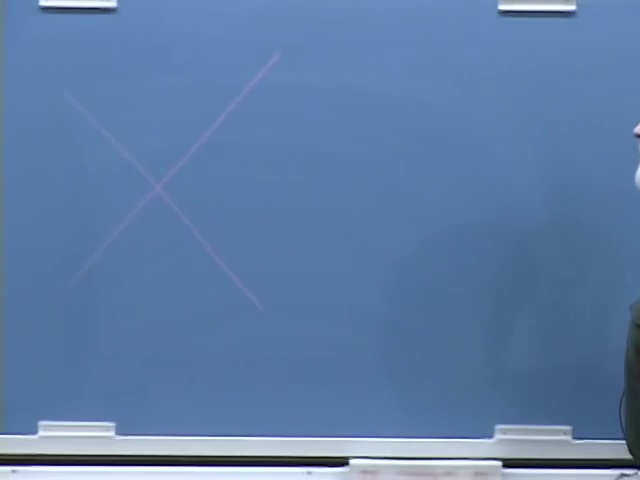
\includegraphics[width=0.68\textwidth]{lecture_09_figure_02.png}
\caption{La temperatura de Hawking \(T_H=1/(8\pi M)\) en unidades naturales.}
\lectureframe{00:08:12}
\end{figure}

Un agujero negro más grande es más frío. La clase lo explica siguiendo hacia atrás la trayectoria de un fotón típico. Los fotones térmicos tienen una energía característica \(E_\gamma\sim T_H\). Un fotón que llega al infinito con una energía del orden de \(M^{-1}\) tenía una energía local mucho mayor cuando se originó cerca del horizonte. El corrimiento al rojo entre la capa cercana al horizonte y el infinito es más intenso en un agujero más grande, por lo que la temperatura asintótica resultante es menor.

\begin{classroomqa}
\audiencequestion{Si el tiempo de Schwarzschild se congela en el horizonte, ¿deberíamos seguir el fotón que cayó originalmente y formó el agujero?\lecturetimestamp{00:04:19}}
\lecturerresponse{Para responder a la pregunta sobre la temperatura, sigamos los fotones emitidos hacia afuera. Se originan con una frecuencia local muy alta, pierden energía al ascender y llegan como radiación de Hawking. El destino del fotón que cayó originalmente es una cuestión distinta, relacionada con la información.}
\end{classroomqa}

\section{La capa de Planck y el horizonte estirado}

¿Hasta qué distancia del horizonte puede confiarse en la relación local de la ecuación~\eqref{eq:l09-local-temperature}? La clase toma la longitud de Planck como la distancia mínima con significado en la descripción semiclásica. Esto sugiere una capa delgada, situada aproximadamente a una longitud de Planck por fuera del horizonte matemático y llena de fluctuaciones a escala de Planck. Emite y absorbe continuamente.

La mayoría de los cuantos emitidos no escapan. Solo los que se dirigen dentro de un cono saliente muy estrecho evitan caer de nuevo. Los cuantos emitidos en direcciones genéricas regresan al horizonte. Las excitaciones salientes y entrantes chocan y producen pares y otras partículas; en este sentido, la descripción estacionaria contiene una capa delgada de material extremadamente caliente.

\begin{figure}[htbp]
\centering
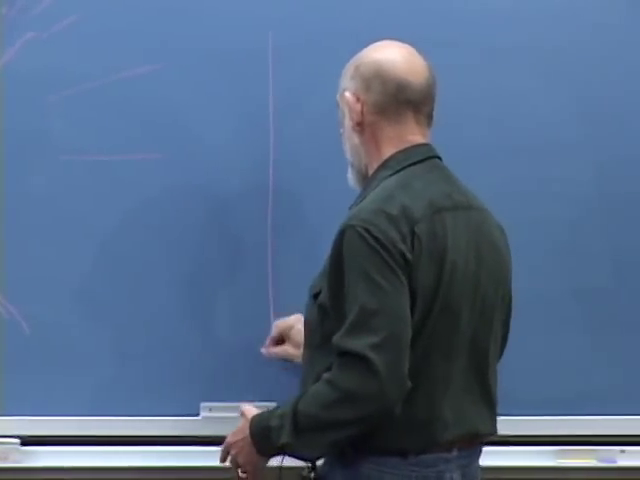
\includegraphics[width=0.74\textwidth]{lecture_09_figure_03.png}
\caption{El estrecho cono de escape de la radiación cercana al horizonte. La mayoría de los cuantos emitidos localmente regresa al horizonte.}
\lectureframe{00:11:38}
\end{figure}

Hay una imagen complementaria del espacio-tiempo. Lejos de un horizonte, una fluctuación virtual puede representarse esquemáticamente mediante un pequeño lazo cerrado: aparece y desaparece una excitación partícula-antipartícula antes de que pueda convertirse en un estado asintótico. Cerca de un horizonte, una fluctuación puede atravesar la frontera causal. Para el observador exterior, la parte que queda fuera parece una partícula emitida por el horizonte y reabsorbida más tarde. Una fracción muy pequeña escapa y se convierte en radiación de Hawking.

\begin{classroomqa}
\audiencequestion{En el diagrama exterior, ¿se extiende una fluctuación de ese tipo desde \(t=-\infty\) hasta \(t=+\infty\)?\lecturetimestamp{00:15:00}}
\lecturerresponse{El horizonte clásico exacto conduce a esa descripción de aspecto singular. En la práctica, lo sustituimos por un horizonte estirado: una superficie temporal situada aproximadamente a una longitud de Planck por fuera. Así, la emisión y la reabsorción ocurren en tiempos exteriores finitos.}
\end{classroomqa}

\begin{figure}[htbp]
\centering
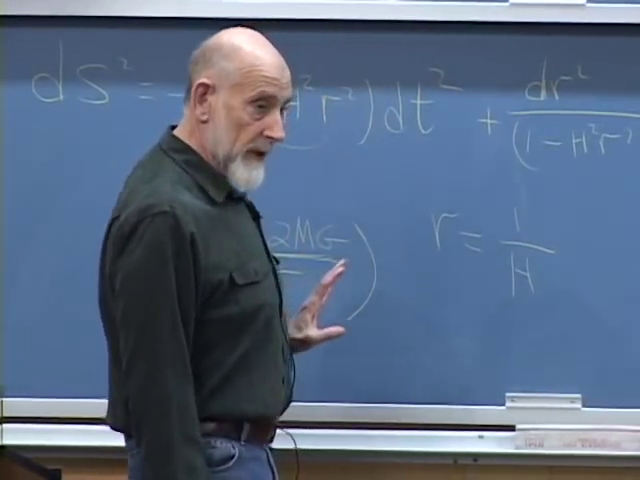
\includegraphics[width=0.72\textwidth]{lecture_09_figure_04.png}
\caption{El horizonte clásico y el horizonte estirado cercano que se usa en la descripción exterior.}
\lectureframe{00:15:52}
\end{figure}

El horizonte estirado no es una nueva frontera invariante. Es una superficie efectiva ubicada donde la geometría semiclásica deja de ser fiable. Las fluctuaciones cuánticas de la materia y de la propia geometría difuminan su ubicación exacta a escalas de Planck. Esta construcción representa esa incertidumbre mediante una superficie en la que la descripción exterior sigue siendo finita.

Nada en este argumento local permite saber si el horizonte pertenece a un agujero negro o a un universo en aceleración. Ese es el puente hacia el espacio de de Sitter.

\section{El espacio de de Sitter en coordenadas de expansión}

La clase formal comienza con la foliación espacialmente plana del espacio-tiempo de de Sitter,
\begin{equation}
ds^2=-dt^2+e^{2Ht}d\mathbf{x}^2,
\qquad
d\mathbf{x}^2=dx^2+dy^2+dz^2.
\label{eq:l09-flat-slicing}
\end{equation}
La constante \(H\) es la tasa de expansión de de Sitter. El factor aparece como \(e^{2Ht}\) porque la métrica mide distancias al cuadrado; un intervalo fijo en las coordenadas tiene una longitud física
\begin{equation}
D(t)=e^{Ht}\lvert\Delta\mathbf{x}\rvert.
\end{equation}

\begin{figure}[htbp]
\centering
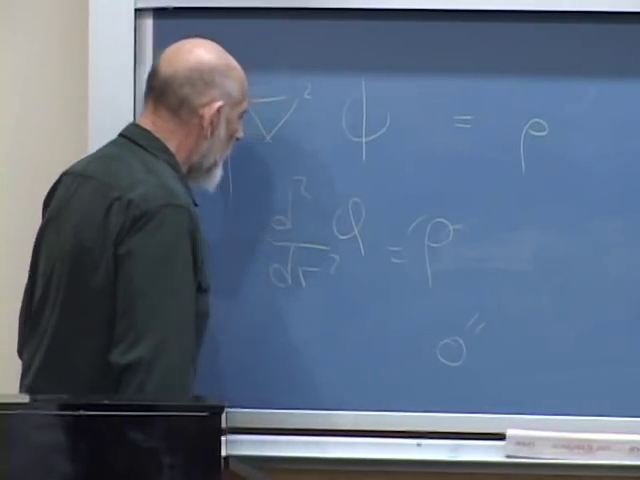
\includegraphics[width=0.78\textwidth]{lecture_09_figure_05.png}
\caption{La métrica de de Sitter, en expansión exponencial y coordenadas planas.}
\lectureframe{00:18:50}
\end{figure}

Estas coordenadas hacen evidente la expansión, pero sitúan el infinito futuro a una distancia infinita hacia arriba en la página. Para llevarlo a la pizarra, introduzcamos el tiempo conforme
\begin{equation}
\eta=-\frac{1}{H}e^{-Ht},
\qquad
-\infty<\eta<0.
\label{eq:l09-conformal-time}
\end{equation}
Entonces
\begin{equation}
dt=\frac{d\eta}{-H\eta},
\qquad
e^{Ht}=-\frac{1}{H\eta},
\end{equation}
y la ecuación~\eqref{eq:l09-flat-slicing} se convierte en
\begin{equation}
ds^2=\frac{1}{H^2\eta^2}
\left(-d\eta^2+d\mathbf{x}^2\right).
\label{eq:l09-conformal-metric}
\end{equation}
Cuando \(t\to+\infty\), \(\eta\to0^{-}\). El tiempo propio infinito se ha comprimido en la línea horizontal finita \(\eta=0\).

\editorialnote{La transformación temporal se corrige varias veces mientras se escribe en la pizarra. La ecuación~\eqref{eq:l09-conformal-time} es la forma coherente: los primeros tiempos cósmicos corresponden a \(\eta\to-\infty\) y el infinito futuro, a \(\eta\to0^{-}\).}

\begin{figure}[htbp]
\centering
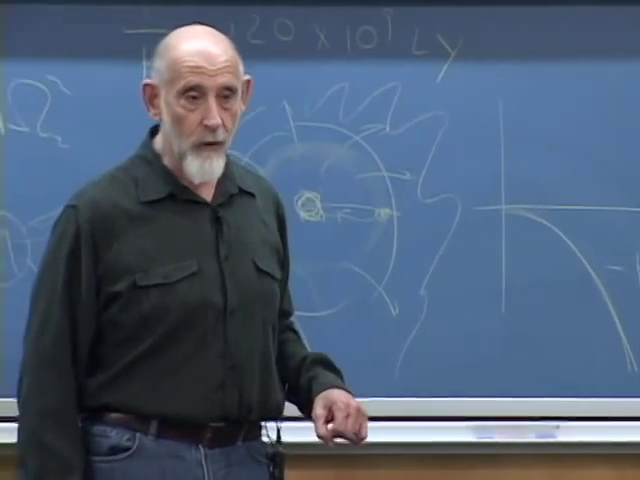
\includegraphics[width=0.82\textwidth]{lecture_09_figure_06.png}
\caption{La transformación al tiempo conforme y la métrica conforme plana.}
\lectureframe{00:21:24}
\end{figure}

El factor conforme multiplica tanto el término temporal como los espaciales, por lo que no altera las direcciones nulas. Para un rayo de luz radial,
\begin{equation}
ds^2=0
\quad\Longrightarrow\quad
-d\eta^2+dx^2=0
\quad\Longrightarrow\quad
\frac{dx}{d\eta}=\pm1.
\label{eq:l09-null-rays}
\end{equation}
Por tanto, la luz viaja a \(45^\circ\) en el diagrama conforme. Por eso resulta útil este cambio de coordenadas: permite visualizar la accesibilidad causal.

\section{La región causal de un observador}

Imaginemos un observador cuya línea de universo continúa durante un tiempo propio infinito. En el diagrama compactificado, termina en un punto de \(\eta=0\). Toda señal que el observador pueda recibir está dentro del cono de luz pasado de ese punto. Los sucesos fuera del cono nunca podrán comunicarse con el observador, por mucho que espere.

\begin{figure}[htbp]
\centering
\includegraphics[width=0.78\textwidth]{lecture_09_figure_07.png}
\caption{El cono de luz pasado límite de un observador en coordenadas conformes de de Sitter.}
\lectureframe{00:24:38}
\end{figure}

Un segundo observador tiene un cono distinto. Las dos regiones accesibles se solapan, pero ninguna abarca todo el espacio-tiempo. Para el resto del argumento, adoptaremos el punto de vista del primer observador y llamaremos región causal del observador a ese cono de luz pasado.

El dibujo parece mostrar cómo la región se contrae hacia el futuro, pero la anchura en coordenadas no es una distancia propia. En una hipersuperficie de \(\eta\), la distancia física al cuadrado entre el observador en \(x=0\) y el horizonte en \(x=\Delta x\) es
\begin{equation}
D^2=\frac{(\Delta x)^2}{H^2\eta^2}.
\label{eq:l09-horizon-distance-start}
\end{equation}
El horizonte es una línea nula a \(45^\circ\) que termina en \(\eta=0\); por tanto,
\begin{equation}
\Delta x=\lvert\eta\rvert.
\end{equation}
Al sustituir se obtiene
\begin{equation}
D_{\rm hor}^2=\frac{1}{H^2},
\qquad
D_{\rm hor}=\frac{1}{H}.
\label{eq:l09-horizon-radius}
\end{equation}
La separación en coordenadas disminuye, pero el factor conforme crece exactamente lo necesario para compensarla. El radio propio del horizonte es constante.

\begin{figure}[htbp]
\centering
\includegraphics[width=0.80\textwidth]{lecture_09_figure_08.png}
\caption{La derivación en la pizarra que convierte el intervalo decreciente en coordenadas en la distancia propia fija \(H^{-1}\).}
\lectureframe{00:28:42}
\end{figure}

\section{La región estática}

Un radio fijo del horizonte sugiere el uso de coordenadas adaptadas al observador central. Sin derivar la transformación de coordenadas, la clase escribe el resultado:
\begin{equation}
ds^2=
-\left(1-H^2r^2\right)d\tau^2
+\frac{dr^2}{1-H^2r^2}
+r^2d\Omega_2^2.
\label{eq:l09-static-patch}
\end{equation}
Los coeficientes dependen de \(r\), no de \(\tau\). Esta carta cubre la región estática del observador,
\begin{equation}
0\le r<\frac{1}{H}.
\end{equation}

\begin{figure}[htbp]
\centering
\includegraphics[width=0.88\textwidth]{lecture_09_figure_09.png}
\caption{La métrica de la región estática de de Sitter y su comparación con el factor de Schwarzschild.}
\lectureframe{00:34:22}
\end{figure}

El parecido con Schwarzschild es inmediato:
\begin{equation}
f_{\rm dS}(r)=1-H^2r^2,
\qquad
f_{\rm Schw}(r)=1-\frac{2G_NM}{r}.
\end{equation}
En ambos casos, el horizonte de las coordenadas estáticas se encuentra donde \(f(r)=0\). Para de Sitter,
\begin{equation}
1-H^2r^2=0
\quad\Longrightarrow\quad
r_H=H^{-1}.
\end{equation}
La carta es singular allí, igual que las coordenadas de Schwarzschild son singulares en el horizonte de un agujero negro. Sin embargo, las geometrías globales difieren en un aspecto importante. Un observador de un agujero negro está fuera y mira hacia dentro; un observador de de Sitter está dentro y mira hacia fuera.

\begin{classroomqa}
\audiencequestion{¿Cómo puede ser estática la geometría si las partículas en caída libre se alejan unas de otras en un universo que se expande exponencialmente?\lecturetimestamp{00:36:06}}
\lecturerresponse{Estático no significa que todas las partículas permanezcan inmóviles. Significa que los coeficientes de la métrica y el resultado de un experimento repetido son independientes del instante de inicio. Si soltamos dos partículas ahora, se aceleran alejándose; si repetimos el mismo experimento más tarde, ocurre el mismo movimiento.}
\end{classroomqa}

\begin{classroomqa}
\audiencequestion{¿Las dos partículas que se alejan la una de la otra se observan mutuamente con corrimiento al rojo?\lecturetimestamp{00:38:34}}
\lecturerresponse{Sí. El aumento de su separación produce un corrimiento al rojo relativo, aunque la métrica adaptada al observador sea independiente del tiempo.}
\end{classroomqa}

\section{La temperatura observada desde el interior}

Las estructuras cercanas al horizonte de Schwarzschild y al de de Sitter son localmente equivalentes. Por tanto, el horizonte de de Sitter emite y reabsorbe cuantos térmicos. Un fotón poco frecuente se propaga hacia el interior hasta el observador central y pierde energía al ascender por el potencial de la región estática. La temperatura de Gibbons--Hawking medida en el centro es
\begin{equation}
T_{\rm dS}=\frac{H}{2\pi}
\label{eq:l09-de-sitter-temperature}
\end{equation}
en unidades naturales. Un termómetro estacionario a un radio \(r\) indica el valor desplazado al rojo de Tolman
\begin{equation}
T_{\rm local}(r)=
\frac{T_{\rm dS}}{\sqrt{1-H^2r^2}},
\label{eq:l09-tolman}
\end{equation}
que diverge cuando \(r\to H^{-1}\) y se reduce, cerca del horizonte, a la ecuación~\eqref{eq:l09-local-temperature}.

\editorialnote{La clase obtiene la escala a partir de la distancia al horizonte y del corrimiento al rojo, en vez de escribir explícitamente las ecuaciones~\eqref{eq:l09-de-sitter-temperature} y \eqref{eq:l09-tolman}. Estas expresan la normalización estándar de ese argumento.}

Para la aceleración tardía observada, la clase emplea la estimación del período
\begin{equation}
H^{-1}\sim 20\times10^9\ {\rm light\ years}.
\label{eq:l09-lecture-horizon-estimate}
\end{equation}
Un fotón típico del horizonte tiene entonces una longitud de onda comparable a miles de millones de años luz. No se trata de radiación de fondo de microondas: es muchísimo más fría.

El experimento mental operacional consiste en una caña de pescar a escala cosmológica. Alicia permanece en \(r=0\), conecta un termómetro a una línea muy larga que también transmite datos y deja que la repulsión cósmica aleje el instrumento. Lo detiene justo antes del horizonte, espera a que vuelva la señal y detecta una temperatura local alta. El termómetro que tiene junto a ella, en el centro, indica el diminuto valor \(H/(2\pi)\). Un mismo horizonte permite ambas lecturas porque se realizan a potenciales gravitatorios distintos.

\section{Cruzar el horizonte}

La descripción clásica desde el exterior se parece a la conocida historia del agujero negro. Bob, situado en el centro, ve alejarse a Alicia. Sus señales sufren un corrimiento al rojo cada vez mayor y llegan cada vez más despacio; ella parece aplanarse contra el horizonte y finalmente se desvanece. Jane, una viajera que llega después, parece formar otra capa más delgada en un estrato sedimentario junto a la frontera.

\begin{classroomqa}
\audiencequestion{Desde nuestro punto de vista, ¿los objetos llegan a atravesar alguna vez el horizonte cósmico?\lecturetimestamp{00:45:30}}
\lecturerresponse{No en la descripción clásica del observador estático. Sus señales sufren un corrimiento al rojo y se desvanecen mientras su posición aparente se aproxima al horizonte. Sin embargo, en su propia descripción en caída libre, lo cruzan sin encontrar una superficie localmente singular.}
\end{classroomqa}

\begin{classroomqa}
\audiencequestion{¿El horizonte solo está caliente para los observadores que permanecen cerca sin cruzarlo? Una observadora en caída libre no se abrasa simplemente por atravesarlo, ¿verdad?\lecturetimestamp{00:48:27}}
\lecturerresponse{Alicia cruza suavemente el horizonte en su propio sistema de referencia. La temperatura extrema pertenece a la descripción estacionaria. Si Bob insiste en observar a Alicia cada vez más cerca del horizonte, tiene que iluminarla con longitudes de onda cada vez más cortas. El microscopio de Heisenberg que intenta usar deposita entonces suficiente energía para abrasar aquello que trata de observar.}
\end{classroomqa}

No hay contradicción entre dos sucesos locales. El observador estacionario y quien cae libre realizan mediciones radicalmente distintas. La complementariedad de horizontes plantea cómo pueden ser válidas ambas descripciones sin permitir que un observador compare directamente información duplicada.

\section{Un modelo newtoniano de la repulsión del vacío}

En este punto, un estudiante pregunta qué reemplaza el pozo gravitatorio del agujero negro. Susskind responde construyendo un modelo newtoniano. Sea \(\phi\) el potencial gravitatorio; la aceleración de una partícula de prueba es
\begin{equation}
\mathbf{a}=-\boldsymbol{\nabla}\phi.
\end{equation}
Para la materia ordinaria no relativista, la ecuación de Poisson es
\begin{equation}
\nabla^2\phi=4\pi G_N\rho.
\label{eq:l09-poisson}
\end{equation}

\begin{classroomqa}
\audiencequestion{Si los efectos del agujero negro se deben a su pozo gravitatorio, ¿cuál es la fuente correspondiente en el espacio de de Sitter?\lecturetimestamp{00:49:36}}
\lecturerresponse{La propia energía del vacío proporciona una fuente gravitatoria espacialmente uniforme. En una descripción newtoniana produce un potencial cuadrático, en lugar de un pozo \(1/r\).}
\end{classroomqa}

\begin{figure}[htbp]
\centering
\includegraphics[width=0.78\textwidth]{lecture_09_figure_10.png}
\caption{La ecuación de Poisson y la forma esquemática de la segunda derivada radial que se usa en la clase.}
\lectureframe{00:51:38}
\end{figure}

En la pizarra se omiten la normalización, los términos asociados a la medida esférica, la presión e incluso, al principio, el signo global, de modo que el ejercicio se reduce a
\begin{equation}
\frac{d^2\phi}{dr^2}\sim H^2.
\end{equation}
La deducción esencial es que una fuente constante da lugar a una función cuadrática. Con el signo necesario para la repulsión de de Sitter,
\begin{equation}
\phi_{\rm dS}(r)=-\frac{1}{2}H^2r^2,
\qquad
a_r=-\frac{d\phi_{\rm dS}}{dr}=H^2r.
\label{eq:l09-de-sitter-potential}
\end{equation}
La aceleración apunta hacia afuera y aumenta linealmente con la distancia. Al resolver \(\ddot r=H^2r\) se obtiene
\begin{equation}
r(\tau)=A e^{H\tau}+B e^{-H\tau},
\end{equation}
y la rama creciente reproduce así la separación exponencial.

\begin{figure}[htbp]
\centering
\includegraphics[width=0.76\textwidth]{lecture_09_figure_11.png}
\caption{La ecuación con fuente uniforme y el potencial cuadrático de de Sitter.}
\lectureframe{00:53:32}
\end{figure}

\editorialnote{En relatividad general, la aceleración en el campo débil de un fluido homogéneo depende de \(\rho+3p\), no solo de \(\rho\). La energía del vacío tiene \(p=-\rho\), de modo que \(\rho+3p=-2\rho\) y la aceleración es repulsiva. La ecuación~\eqref{eq:l09-de-sitter-potential} es el resultado de de Sitter con la normalización correcta; el cálculo en la pizarra sigue deliberadamente solo la dependencia cuadrática y el signo.}

Coloquemos una masa ordinaria \(M\) en el centro. El potencial cualitativo pasa a ser
\begin{equation}
\phi(r)=-\frac{G_NM}{r}-\frac{1}{2}H^2r^2,
\label{eq:l09-combined-potential}
\end{equation}
y la aceleración radial es
\begin{equation}
a_r=-\frac{G_NM}{r^2}+H^2r.
\end{equation}
A valores pequeños de \(r\) domina la atracción local; a valores grandes de \(r\) domina la repulsión del vacío. El equilibrio se produce en
\begin{equation}
r_\ast=\left(\frac{G_NM}{H^2}\right)^{1/3}.
\label{eq:l09-turnaround}
\end{equation}
Esta es la versión clara del máximo del potencial que presenta la clase. Explica cualitativamente por qué los sistemas ligados por la gravedad pueden permanecer unidos en las proximidades, mientras que las galaxias suficientemente lejanas se alejan con aceleración.

\begin{figure}[htbp]
\centering
\includegraphics[width=0.78\textwidth]{lecture_09_figure_12.png}
\caption{La atracción ordinaria \(1/r\) combinada con el potencial cuadrático invertido de de Sitter.}
\lectureframe{00:58:20}
\end{figure}

\begin{classroomqa}
\audiencequestion{¿Siguen siendo importantes las fuerzas ordinarias o la repulsión del vacío acabará desgarrando todas las agrupaciones de materia?\lecturetimestamp{00:57:29}}
\lecturerresponse{Hay que tener en cuenta todas las fuerzas. A escalas suficientemente pequeñas predominan la interacción electromagnética que mantiene unidos los sistemas y la gravedad local. La repulsión del vacío solo cobra importancia a distancias enormes, determinadas por \(H^{-1}\) y por la escala de equilibrio que corresponde a la masa ligada.}
\end{classroomqa}

\section{Una fuente, varios nombres}

La discusión se detiene ahora en la terminología. En el modelo que usamos, la energía del vacío, la constante cosmológica y la energía oscura no son tres sustancias aditivas. Son tres descripciones de la misma fuente \(w=-1\). Puede hablarse de un término constante en la ecuación de Einstein, de una densidad de energía del vacío invariante de Lorentz o del componente que impulsa la aceleración tardía.

\begin{classroomqa}
\audiencequestion{¿Están presentes a la vez la fuente newtoniana uniforme y la energía cuántica del vacío como efectos separados?\lecturetimestamp{00:59:14}}
\lecturerresponse{No. La densidad uniforme es el modelo newtoniano de esa misma fuente. En esta clase, energía del vacío, constante cosmológica y energía oscura se refieren a un único componente físico.}
\end{classroomqa}

\begin{classroomqa}
\audiencequestion{¿Tiene entonces el mismo fenómeno una descripción clásica y otra cuántica?\lecturetimestamp{01:00:32}}
\lecturerresponse{Su origen microscópico puede ser mecánico-cuántico, del mismo modo que parte de la masa del electrón tiene un origen cuántico. Una vez conocida la densidad de energía efectiva, esta entra en las ecuaciones clásicas de la gravedad como una fuente ordinaria. Desconocemos el origen último del valor observado.}
\end{classroomqa}

En unidades de Planck, la densidad de energía del vacío observada es extraordinariamente pequeña,
\begin{equation}
\rho_\Lambda\sim10^{-123}\rho_{\rm Pl},
\label{eq:l09-planck-smallness}
\end{equation}
hasta el factor convencional que se use para la densidad de Planck. Ese número tan pequeño constituye el problema de la constante cosmológica. También explica por qué el horizonte es tan grande: en cuatro dimensiones,
\begin{equation}
H^2=\frac{8\pi G_N}{3}\rho_\Lambda,
\qquad
r_H=H^{-1}.
\end{equation}
Si \(H\) fuera mayor, el horizonte sería menor, la temperatura central de de Sitter sería mayor y la aceleración repulsiva \(H^2r\) sería más intensa.

\begin{classroomqa}
\audiencequestion{¿Está relacionada la diminuta constante cosmológica con la constante de Planck y las fluctuaciones cuánticas?\lecturetimestamp{01:03:27}}
\lecturerresponse{La comparación más clara emplea unidades de Planck adimensionales, en las que \(G_N=\hbar=c=1\). En esas unidades, la densidad del vacío es unos \(123\) órdenes de magnitud menor que la densidad de Planck natural. Explicar esa jerarquía es uno de los problemas centrales de la física fundamental.}
\end{classroomqa}

\begin{classroomqa}
\audiencequestion{¿Tiene que ser la energía del vacío una constante cosmológica exactamente constante? ¿Podría disminuir el componente acelerado y acabar estabilizándose en cero?\lecturetimestamp{01:04:52}}
\lecturerresponse{Esa es una alternativa lógicamente posible: un campo dinámico de energía oscura podría variar con el tiempo. La clase adopta el caso constante porque las observaciones disponibles en aquel momento favorecían cada vez más un comportamiento cercano al de una constante cosmológica, no porque se hubiera demostrado imposible toda alternativa.}
\end{classroomqa}

\section{La astronomía en un futuro lejano}

En un universo que tiende asintóticamente al espacio de de Sitter, las estructuras que no están ligadas gravitatoriamente acaban cruzando el horizonte del observador. El fondo cósmico de microondas se desplaza al rojo hasta dejar de ser detectable. Las galaxias lejanas desaparecen. Un astrónomo que sobreviva quizá solo vea una agrupación gravitatoria local fusionada, dentro de una región por lo demás oscura.

\begin{classroomqa}
\audiencequestion{Sin telescopio, ¿alguien siquiera notaría que han desaparecido las galaxias lejanas?\lecturetimestamp{01:06:17}}
\lecturerresponse{Probablemente no. El problema de fondo es más profundo: incluso con instrumentos avanzados, quizá los observadores futuros carezcan de los trazadores distantes y del fondo de microondas que hoy nos permiten inferir la expansión.}
\end{classroomqa}

Entonces podría parecer convincente la antigua imagen de un universo de islas. La paradoja de Olbers no obligaría a llegar a otra conclusión, porque presupone una población infinita, estática y uniforme de fuentes luminosas; el observador del futuro solo vería las estrellas finitas de la agrupación local. La energía oscura no crea continuamente galaxias de reemplazo a partir del espacio vacío.

El horizonte del espacio de de Sitter exacto no se contrae alrededor de la galaxia local. Su radio físico permanece en \(H^{-1}\), un valor muchísimo mayor que el tamaño de una galaxia. Lo que desaparece es la materia no ligada que atraviesa esa frontera causal fija.

\begin{classroomqa}
\audiencequestion{¿Podrían las estrellas expulsadas de la galaxia servir como cuerpos de prueba para detectar la geometría a gran escala?\lecturetimestamp{01:11:25}}
\lecturerresponse{Durante un tiempo, sí. Los objetos expulsados y las señales luminosas de gran alcance podrían explorar la geometría. Pero el efecto solo se vuelve apreciable a distancias del orden de una fracción considerable de mil millones de años luz, por lo que el experimento requeriría tiempos cosmológicos.}
\end{classroomqa}

\begin{classroomqa}
\audiencequestion{¿Cómo sabemos que un horizonte lejano no nos ha ocultado ya la mayor parte del universo?\lecturetimestamp{01:11:45}}
\lecturerresponse{Ya vemos suficientes galaxias, corrimientos al rojo y radiación de fondo para medir la expansión y reconstruir la geometría a gran escala. Los observadores futuros privados de esos trazadores se enfrentarían a un problema de inferencia mucho más difícil.}
\end{classroomqa}

\begin{classroomqa}
\audiencequestion{Si el horizonte estuviera justo más allá de Andrómeda, ¿sería evidente su presencia?\lecturetimestamp{01:12:19}}
\lecturerresponse{Sí. Un horizonte tan pequeño requeriría un valor mucho mayor de \(H\), y la repulsión resultante alteraría considerablemente el movimiento de Andrómeda. El valor medido sitúa, en cambio, el horizonte asintótico a una escala inmensamente mayor.}
\end{classroomqa}

\begin{classroomqa}
\audiencequestion{¿Podrían estar ocurriendo nuevos Big Bangs más allá de nuestro horizonte?\lecturetimestamp{01:13:25}}
\lecturerresponse{Los sucesos que ocurren más allá del horizonte no son visibles para nosotros ni para nuestros descendientes. Más adelante en la clase se presentará una posibilidad relacionada, pero más precisa: la nucleación de burbujas en la inflación eterna.}
\end{classroomqa}

Con cohetes, relojes y varios miles de millones de años, los observadores futuros podrían enviar exploradores a través de una gran parte de la región y reconstruir su métrica. Sin embargo, en escalas de tiempo propias de un laboratorio o de una civilización, el efecto es casi inaccesible. Esta distinción corrige la afirmación excesiva de que sería imposible descubrir la expansión: está fuera del alcance práctico inmediato, pero no está prohibida en principio.

\begin{classroomqa}
\audiencequestion{¿Podrían los exploradores futuros determinar la geometría mucho antes de tener que esperar una recurrencia térmica?\lecturetimestamp{01:21:40}}
\lecturerresponse{Desde luego. No se propone medirla esperando una recurrencia. Los exploradores podrían cartografiar la región estática intercambiando señales luminosas a lo largo de distancias de miles de millones de años luz; tardarían muchísimo menos, aunque todavía necesitarían tiempos cosmológicos.}
\end{classroomqa}

\begin{classroomqa}
\audiencequestion{¿El corrimiento al rojo borraría toda la información que obtuvieran exploradores de ese tipo?\lecturetimestamp{01:23:24}}
\lecturerresponse{No, si exploran escalas muy inferiores al horizonte. Una línea de base del orden de mil millones de años luz ya es sensible a la expansión y produce solo un corrimiento al rojo moderado. El experimento está limitado, sobre todo, por su duración inmensa.}
\end{classroomqa}

\section{Entropía finita y recurrencia}

El parche estático no está vacío en sentido termodinámico. Su horizonte tiene un área
\begin{equation}
A_H=4\pi H^{-2},
\end{equation}
una temperatura \(T_{\rm dS}=H/(2\pi)\) y una entropía
\begin{equation}
S_{\rm dS}=\frac{A_H}{4G_N}
=\frac{\pi}{G_NH^2}
\label{eq:l09-de-sitter-entropy}
\end{equation}
en unidades \(\hbar=c=k_B=1\). La entropía es finita. Por tanto, con las debidas cautelas, se puede imaginar el parche estático como una cavidad térmica de entropía finita, cuyas excitaciones se concentran cerca del horizonte en la descripción estacionaria.

Una caja ordinaria de gas en equilibrio parece no tener estructura en escalas de tiempo cortas, pero la mecánica estadística no prohíbe las fluctuaciones. Si un macroestado tiene un déficit de entropía \(\Delta S\) respecto del equilibrio, su probabilidad es aproximadamente
\begin{equation}
P\sim e^{-\Delta S}.
\label{eq:l09-fluctuation-probability}
\end{equation}
El tiempo de espera correspondiente crece como
\begin{equation}
t\sim t_0 e^{\Delta S}.
\end{equation}
En un sistema finito, el tiempo necesario para volver a un estado arbitrariamente cercano a uno anterior es el tiempo de recurrencia de Poincaré,
\begin{equation}
t_{\rm rec}\sim H^{-1}e^{S_{\rm dS}}.
\label{eq:l09-recurrence}
\end{equation}
Como \(S_{\rm dS}\) de nuestro horizonte es del orden de \(10^{120}\), la clase resume la escala como \(e^{10^{120}}\). Es irrelevante si el prefactor se mide en años, tiempos de Hubble o unidades microscópicas, frente a la doble exponencial.

\begin{figure}[htbp]
\centering
\includegraphics[width=0.76\textwidth]{lecture_09_figure_13.png}
\caption{La discusión sobre recurrencia, con la enorme escala exponencial del tiempo de espera escrita en la pizarra.}
\lectureframe{01:16:24}
\end{figure}

Antes de una recurrencia semejante, las fluctuaciones menores son muchísimo más frecuentes. Todas las moléculas de una habitación podrían reunirse en una esquina; podría formarse brevemente un vórtice complicado; en la jerarquía jocosa de la clase, el movimiento térmico podría ensamblar un elefante. Cuanto menor sea el déficit de entropía requerido, menos costosa será la fluctuación.

\begin{classroomqa}
\audiencequestion{¿Las recurrencias de Poincaré son específicamente una consecuencia de la mecánica cuántica?\lecturetimestamp{01:25:44}}
\lecturerresponse{No. La recurrencia y las fluctuaciones raras ya aparecen en la mecánica estadística clásica. Su aplicación al espacio de de Sitter se basa en nuestro marco físico actual, que quizá algún día se revise, pero la termodinámica y el razonamiento estadístico se cuentan entre las estructuras más sólidas que conocemos.}
\end{classroomqa}

El significado mismo de la probabilidad podría profundizarse en una teoría futura. Susskind no afirma lo contrario. Su planteamiento, más acotado, es que abandonar la mecánica estadística solo porque sus implicaciones a largo plazo resultan extrañas supondría descartar uno de los principios organizadores mejor comprobados de la física.

\section{Cerebros de Boltzmann y observadores típicos}

Supongamos que una fluctuación térmica crea un estado entero semejante al big bang. Eso requiere una disminución enorme de la entropía. Una fluctuación que produzca un sistema solar cuesta menos; una que produzca una Tierra ya cálida, menos aún. Si el único requisito es que haya un observador, la fluctuación menos costosa quizá solo crearía un cerebro funcional con recuerdos aparentes. A ese observador hipotético se le llama cerebro de Boltzmann.

La cuestión no es si una fluctuación extravagante es lógicamente posible. La cuestión es si un modelo cosmológico predice que casi todos los observadores son fluctuaciones de ese tipo. Inferimos a partir de nuestras observaciones suponiendo que no somos extraordinariamente atípicos. Una teoría en la que los observadores ordinarios, con historias cósmicas coherentes, quedan superados exponencialmente en número por cerebros térmicos aislados socava esa inferencia.

Por tanto, el problema de los cerebros de Boltzmann plantea una prueba cuantitativa de consistencia. Se compara la abundancia esperada de observadores ordinarios con la de observadores surgidos de fluctuaciones. Si predominan estos últimos, habrá que concluir que el vacío debe decaer antes de que proliferen, que hay que cambiar la medida o que deben reconsiderarse los supuestos cosmológicos.

Se deja explícitamente para más adelante una pregunta anterior sobre una conexión entre el ultravioleta--el infrarrojo. El argumento de recurrencia no depende de resolver esa cuestión aparte.

\section{Inflación eterna y universos burbuja}

A continuación, la clase introduce un segundo problema de probabilidad, sin intentar derivarlo por completo. En un vacío metastable de de Sitter puede nuclearse una burbuja cuyo vacío tiene menor energía. La pared de la burbuja se expande y el interior puede evolucionar hasta convertirse en un universo de Friedmann--Robertson--Walker abierto. Mientras tanto, la región inflacionaria circundante sigue expandiéndose y nuclea más burbujas.

\begin{figure}[htbp]
\centering
\includegraphics[width=0.74\textwidth]{lecture_09_figure_14.png}
\caption{Una burbuja con menor energía del vacío dibujada dentro de un fondo de de Sitter en inflación.}
\lectureframe{01:29:38}
\end{figure}

La característica crucial es el crecimiento exponencial de la población. Se produce nuevo volumen físico más deprisa de lo que las burbujas lo eliminan, así que el número de regiones burbuja crece sin límite. Distintas burbujas pueden asentarse en estados de baja energía diferentes y, por tanto, presentar una física efectiva distinta.

Para exponer la dificultad estadística, Susskind deja primero la cosmología y considera una población humana en crecimiento exponencial con recursos finitos, pero desconocidos. Supongamos que los observadores son típicos entre todas las personas que llegarán a vivir. Si la población se duplica en cada generación y luego desaparece, la mitad de todas las personas vivirá en la última generación, tres cuartas partes en las dos últimas y siete octavas partes en las tres últimas:
\begin{equation}
f_n=1-2^{-n}.
\label{eq:l09-last-generations}
\end{equation}
La tipicidad nos situaría entonces incómodamente cerca del final, aunque no sepamos nada sobre la cantidad total de recursos. Esto no se ofrece como una predicción fiable de la extinción humana. Es una advertencia: el crecimiento exponencial hace que los recuentos estén dominados por el corte.

El ejemplo de quienes lanzan monedas expresa con más claridad la suposición habitual de tipicidad. Si muchos experimentadores lanzan cada uno una moneda equilibrada \(N\) veces, la inmensa mayoría obtiene
\begin{equation}
n_H=\frac{N}{2}+O(\sqrt{N}).
\end{equation}
Un observador con un resultado extremo debería sospechar primero que el modelo o la moneda son defectuosos, en vez de suponer sin pruebas que ocupa una cola extraordinariamente rara. La probabilidad cosmológica parte de la misma intuición sobre la tipicidad, pero en una población infinita necesita un método de recuento bien definido.

\section{El límite de Escher y el problema de la medida}

La analogía geométrica de Susskind es \ M.\ C.\emph{Circle Limit IV}, de Escher: el disco teselado con ángeles y demonios que parecen más pequeños al acercarse al borde. En la geometría hiperbólica representada por el dibujo, las figuras son equivalentes; su tamaño euclidiano aparente solo cambia debido a la proyección.

\begin{figure}[htbp]
\centering
\includegraphics[width=0.76\textwidth]{lecture_09_figure_15.png}
\caption{El sustituto en la pizarra de las figuras de Escher que proliferan exponencialmente cerca de un límite circular.}
\lectureframe{01:37:54}
\end{figure}

Imaginemos que Escher dispone de tiempo, tinta y paciencia finitos. Al acercarse al borde, acaba por detenerse, quizá dejando algunas figuras incompletas. Como el número de figuras crece exponencialmente con el radio hiperbólico, una capa exterior de grosor finito contiene una fracción fija de todas las figuras dibujadas. Aproximadamente la mitad puede quedar en la capa final, por lejos que se desplace hacia fuera el corte.

Preguntemos ahora por la proporción entre ángeles y demonios. En el patrón infinito ideal, la simetría sugiere una igualdad uno a uno. Sin embargo, en cualquier recuento finito, un límite ligeramente distinto puede incluir muchas más figuras de un tipo. Como la mayor parte del recuento se concentra cerca del límite, una pequeña deformación de este produce un cambio de orden uno en el resultado.

\begin{figure}[htbp]
\centering
\includegraphics[width=0.76\textwidth]{lecture_09_figure_16.png}
\caption{En un patrón de crecimiento exponencial, el límite de corte domina el recuento.}
\lectureframe{01:43:06}
\end{figure}

La misma ambigüedad aparece en la inflación eterna. Se cuentan los universos burbuja azules y rosas por debajo de cierto corte temporal y luego se desplaza el corte hacia tiempos posteriores. Ambos recuentos divergen, y su proporción puede depender mucho de qué significa \emph{tiempo} y de cómo se trace la superficie de corte. Una medida de probabilidad es una prescripción que regula la población infinita y extrae probabilidades relativas. Que distintas prescripciones plausibles no coincidan constituye el problema de la medida.

\begin{classroomqa}
\audiencequestion{¿Hay alguna relación entre este problema del corte y la renormalización?\lecturetimestamp{01:45:43}}
\lecturerresponse{Hay una analogía. En teoría cuántica de campos se introduce una retícula o un corte ultravioleta, se refina y se buscan magnitudes insensibles a los detalles del borde del regulador. Los cosmólogos esperan obtener una extracción igual de robusta de la inflación eterna, pero en el marco que se analiza aquí todavía no hay una prescripción de solidez comparable.}
\end{classroomqa}

No conviene llevar demasiado lejos la analogía. La renormalización funciona cuando un flujo controlado identifica observables independientes del regulador. El problema de la medida consiste precisamente en que no están claras las preguntas invariantes análogas ni el procedimiento límite. Decir que quizá estamos planteando la pregunta equivocada no resuelve nada mientras no se formule la pregunta correcta.

\begin{classroomqa}
\audiencequestion{¿Esta imagen de burbujas es el mismo fenómeno que la inflación de nuestro universo temprano?\lecturetimestamp{01:48:19}}
\lecturerresponse{Está estrechamente relacionada. En la inflación eterna, el fondo progenitor sigue inflándose mientras los interiores de las burbujas locales atraviesan su propia evolución cosmológica. Nuestro universo observable podría estar dentro de una región semejante.}
\end{classroomqa}

\section{¿Podrían observarse colisiones entre burbujas?}

Cuando dos burbujas se encuentran, sus energías del vacío no se suman sin más. Una pared de dominio separa regiones con distintos estados del vacío, y la geometría de la pared determina qué puede observar cada lado. Según dónde se produzca la colisión con respecto a nuestro cono de luz pasado, su huella podría quedar oculta o ser visible.

\begin{classroomqa}
\audiencequestion{¿Qué ocurre cuando colisionan dos burbujas de vacío?\lecturetimestamp{01:52:07}}
\lecturerresponse{La colisión genera una geometría de pared de dominio cuyo comportamiento depende de los dos vacíos y de la tensión de la pared. En circunstancias causales favorables, la perturbación puede entrar en nuestra región observable y dejar una señal anisótropa.}
\end{classroomqa}

La clase analiza una región fría del fondo cósmico de microondas como posible candidata y señala la polarización alrededor de una estructura circular como elemento discriminante. Se presenta deliberadamente como una posibilidad, no como una detección. Una señal convincente de una colisión sería revolucionaria, porque aportaría evidencia directa de regiones burbuja vecinas y haría urgente desde el punto de vista experimental el problema de la medida.

\begin{figure}[htbp]
\centering
\includegraphics[width=0.70\textwidth]{lecture_09_figure_17.png}
\caption{Una estructura circular en el cielo y su posible patrón de polarización en la discusión sobre colisiones de burbujas.}
\lectureframe{01:50:22}
\end{figure}

\editorialnote{La discusión sobre la mancha fría recoge el estado de las observaciones y las propuestas vigentes en el momento de la clase. Una anomalía de temperatura por sí sola no constituye evidencia de una colisión de burbujas; haría falta una señal detallada y correlacionada.}

\begin{classroomqa}
\audiencequestion{¿Las burbujas son tetradimensionales y qué curvatura espacial tienen sus interiores?\lecturetimestamp{01:53:37}}
\lecturerresponse{Son regiones del espacio-tiempo, no burbujas de jabón tridimensionales que evolucionan en un tiempo externo. Sus interiores suelen ser universos FRW abiertos con curvatura espacial negativa. Una colisión perturba esa geometría, pero no convierte sin más la curvatura negativa en positiva.}
\end{classroomqa}

\section{Qué establece la teoría de cuerdas y qué no}

La discusión final comienza con una invitación a asignar una probabilidad de que la teoría de cuerdas sea correcta. Susskind se niega a dar una cifra porque la proposición es demasiado ambigua. En su lugar, distingue dos afirmaciones.

En primer lugar, existe una estructura matemática muy restringida que combina la mecánica cuántica y la gravedad. Ha producido resultados precisos e identidades matemáticas profundas, y su consistencia interna ha resistido un examen exhaustivo. En el vocabulario informal de la clase, esto es \emph{la Teoría de Cuerdas} con mayúscula \(S\). Las versiones que mejor se comprenden dependen en gran medida de la supersimetría.

En segundo lugar, el mundo observado no es supersimétrico a las energías accesibles. Conectar las construcciones supersimétricas exactas con nuestro universo no supersimétrico requiere la ruptura de la supersimetría y un marco más amplio que no está controlado con la misma precisión. En el vocabulario de la clase, esa extensión esperada es \emph{la teoría de cuerdas} con minúscula \(s\).

\begin{classroomqa}
\audiencequestion{¿Se puede asignar una probabilidad de que la teoría de cuerdas sea la teoría correcta de la naturaleza?\lecturetimestamp{01:54:18}}
\lecturerresponse{No sería responsable hacerlo sin especificar a cuál de las afirmaciones nos referimos. Las estructuras matemáticas exactas existen e incluyen la gravedad cuántica, pero los modelos supersimétricos bajo control riguroso no son literalmente el mundo que observamos. Que una extensión más amplia contenga nuestro mundo es una cuestión sobre la que los físicos pueden tener opiniones informadas, pero no admite una probabilidad numérica bien definida.}
\end{classroomqa}

La analogía es con la mecánica, antes de que se dispusiera de todo el aparato matemático. Se podrían conocer \(F=ma\) y la fuerza inversamente proporcional al cuadrado de la distancia, pero solo ser capaz de resolver órbitas circulares con mucha simetría. El sector resoluble sería auténtico, pero no abarcaría toda la teoría. Del mismo modo, las construcciones exactas de teoría de cuerdas supersimétrica podrían ser una región especial, inusualmente tratable, de una estructura más amplia.

\begin{figure}[htbp]
\centering
\includegraphics[width=0.60\textwidth]{lecture_09_figure_18.png}
\caption{La imagen anidada de la clase: construcciones de teoría de cuerdas supersimétrica bajo control riguroso dentro de un marco que, según la conjetura, sería más amplio.}
\lectureframe{01:57:34}
\end{figure}

\begin{classroomqa}
\audiencequestion{¿Por qué no romper simplemente la supersimetría en la teoría exacta?\lecturetimestamp{01:57:02}}
\lecturerresponse{Muchas construcciones aproximadas estudian la ruptura de la supersimetría, pero lo que falta precisamente es una estructura fundamental no supersimétrica bajo control completo. Se pueden hacer cálculos con aproximaciones habituales sin saber siempre a qué objeto exacto se aproximan.}
\end{classroomqa}

\begin{classroomqa}
\audiencequestion{¿La teoría supersimétrica exacta descarta una extensión más amplia y menos simétrica que contenga nuestro mundo?\lecturetimestamp{02:00:33}}
\lecturerresponse{No. Establece que el mundo observado no queda descrito únicamente por el sector supersimétrico exacto. No demuestra ni refuta que ese sector esté conectado con una teoría más amplia que contenga física realista.}
\end{classroomqa}

\begin{classroomqa}
\audiencequestion{¿Las construcciones de teoría de cuerdas incluyen una ruptura de simetría análoga a la ruptura de simetría en física de partículas?\lecturetimestamp{02:01:21}}
\lecturerresponse{Hay abundante trabajo sobre la ruptura de la supersimetría y se conoce mucho de las matemáticas supersimétricas. La cuestión sin resolver es cómo formular con precisión y de manera no perturbativa una teoría que combine una ruptura realista con la teoría completa, y no solo con aproximaciones controladas.}
\end{classroomqa}

\begin{classroomqa}
\audiencequestion{¿La relatividad especial se postula en la teoría de cuerdas o surge como predicción?\lecturetimestamp{02:03:02}}
\lecturerresponse{Las reglas fundamentales son invariantes de Lorentz, aunque un fondo particular lleno de materia pueda seleccionar un sistema de referencia en reposo preferente. La gravedad es aún más inevitable: el espectro de cuerdas contiene una excitación sin masa de espín dos, con las interacciones de un gravitón.}
\end{classroomqa}

\begin{classroomqa}
\audiencequestion{¿Es compatible la teoría de cuerdas con la relatividad general y la independencia del fondo?\lecturetimestamp{02:04:11}}
\lecturerresponse{Su dinámica gravitatoria de baja energía es compatible con la relatividad general, y los fondos locales pueden cambiar dinámicamente. La sutileza reside en las condiciones de contorno asintóticas: estas definen el problema y, en general, no pueden cambiarse mediante una operación local dentro de ese espacio-tiempo.}
\end{classroomqa}

La clase concluye con esa distinción entre un núcleo matemático sólido y una extrapolación física aún incompleta. No es un veredicto de que el núcleo sea inútil ni afirma que la extrapolación esté establecida. Señala hasta dónde llega el conocimiento exacto.
\end{document}
